\documentclass[compsoc]{IEEEtran}

%%%%%%% USE PACKAGES %%%%%%%
\usepackage{cite}
\usepackage{amsmath, amsfonts, amsthm, amssymb}  % Some math symbols
\usepackage{enumerate}
\usepackage{enumitem}
\usepackage{hyperref}
\usepackage{algorithmic}
\usepackage{graphicx}
\usepackage{textcomp}
\usepackage{xcolor}
\usepackage{natbib}
\usepackage{wrapfig}
\usepackage{changepage}
\usepackage{subfig}
\usepackage{float}
\usepackage{setspace}
\usepackage{hhline}
\usepackage{makecell}
\usepackage[all]{xy}
\usepackage{fancyvrb}
\usepackage[T1]{fontenc}
\usepackage{listings}
\usepackage{fancyhdr}
\usepackage{mathtools}
\usepackage{capt-of}
\usepackage{gensymb}
\usepackage{epstopdf}
\usepackage{booktabs}
\usepackage{centernot}
\usepackage{titlesec}
\usepackage[pdftex]{hyperref}
\usepackage{tocloft}
\usepackage{multirow}
\usepackage{advdate}    % Advancing/saving dates
\usepackage{datetime}   % Dates formatting
\usepackage{datenumber} % Counters for dates
\usepackage[table]{xcolor}
\usepackage{array}
\usepackage{tikz}
\usepackage{pgfgantt}
\usepackage{rotating}
\usepackage[graphicx]{realboxes}
\usepackage{hvfloat}
\usepackage{tcolorbox}
\usepackage{tabularx} 
\usepackage{placeins}
\usepackage[separate-uncertainty = true, multi-part-units = repeat]{siunitx}
\usetikzlibrary{shapes,arrows}

%%%%%%% CONFIGURATION %%%%%%%
\usetikzlibrary{positioning}

\renewcommand{\sfdefault}{ppl}

\pagestyle{fancy}
\fancyhf{}
\renewcommand{\headrulewidth}{0pt}
\cfoot{\thepage}

\DeclarePairedDelimiter{\ceil}{\lceil}{\rceil}
\DeclarePairedDelimiter{\floor}{\lfloor}{\rfloor}
\DeclarePairedDelimiter{\card}{\vert}{\vert}

\usepackage[style=ieee]{biblatex}
\DeclareLanguageMapping{english}{english-apa}
\addbibresource{references.bib}

\def\BibTeX{{\rm B\kern-.05em{\sc i\kern-.025em b}\kern-.08em
    T\kern-.1667em\lower.7ex\hbox{E}\kern-.125emX}}

% \pagestyle{head}
\setlength{\parindent}{0pt}
\setlength{\parskip}{11pt}

%%%%%%% ONE COLUMN %%%%%%% 
\onecolumn
\raggedbottom

%%%%%%% VARIABLES %%%%%%%
\newcommand{\cc}[1]{\texttt{#1}}

\newcommand{\studentOneName}{Aswani, Nishant}
\newcommand{\studentTwoName}{Simsek, Barkin}
\newcommand{\studentOneEmail}{nsa325@nyu.edu}
\newcommand{\studentTwoEmail}{bs3528@nyu.edu}
\newcommand{\advisorOneName}{Karau, Matt}
\newcommand{\advisorTwoName}{Jabari, Saif E.}
\newcommand{\group}{Group 7}

%%%%%%% \thickhline for tables %%%%%%%
\makeatletter
\def\thickhline{%
  \noalign{\ifnum0=`}\fi\hrule \@height \thickarrayrulewidth \futurelet
   \reserved@a\@xthickhline}
\def\@xthickhline{\ifx\reserved@a\thickhline
               \vskip\doublerulesep
               \vskip-\thickarrayrulewidth
             \fi
      \ifnum0=`{\fi}}
\makeatother

\newlength{\thickarrayrulewidth}
\setlength{\thickarrayrulewidth}{3\arrayrulewidth}

%%%%%%% TUNABLES %%%%%%%
\setlength{\cftbeforesecskip}{7pt}
\setlength{\cftbeforesubsecskip}{7pt}
\setlength{\cftbeforesubsubsecskip}{7pt}

\setcounter{tocdepth}{3}
\hypersetup{colorlinks,linkcolor=,urlcolor=links}

\titlespacing\section{0pt}{12pt plus 4pt minus 2pt}{0pt plus 2pt minus 2pt}
\titlespacing\subsection{0pt}{12pt plus 4pt minus 2pt}{0pt plus 2pt minus 2pt}
\titlespacing\subsubsection{0pt}{12pt plus 4pt minus 2pt}{0pt plus 2pt minus 2pt}

\setlength{\belowcaptionskip}{-10pt}



\begin{document}

%%%%%%% COVER PAGE %%%%%%%
\begin{titlepage}

 \begin{center}
 \textbf{\large Senior Capstone Project}
       \vspace*{\fill}

        \textbf {Capstone Final Report\\}
        \vspace{10pt}
        \textbf {\large ramen: Design and Development of a Raft Consensus Algorithm \\Coupled With a IEEE 802.11 Based Mesh Network for Embedded Systems\\}
        \vspace{10pt}
        \today
      
        \vfill
            
     \underline {Advisors:}\\
       \advisorOneName\\
       \advisorTwoName\\
       
            
       \vspace{0.8cm}
     
    %   \includegraphics[width=0.4\textwidth]{university}
            
       \underline {\group}\\
       \studentOneName - \studentOneEmail\\
       \studentTwoName - \studentTwoEmail\\
      
            
   \end{center}
\end{titlepage}

%%%%%%% TABLE OF CONTENTS %%%%%%%
\tableofcontents

%%%%%%% REPORT BEGINNING %%%%%%%
\newpage
\setstretch{1.25}

%%%%%%% ABSTRACT %%%%%%%
\section{Abstract}
% Used to indicate where a new paragraph starts within the abstract 
\newcommand{\nextInternalParagraphStartsHere}{}

Consensus is a fundamental problem in fault-tolerant distributed systems and involves multiple nodes arriving at a coordinated decision. Reaching a consensus is more challenging if the system is dynamic and if it makes decisions in real-time, as is the case with autonomous vehicles and mobile sensor networks. Thus, consensus algorithms ensure that a cluster of devices can cooperatively complete its tasks even if the cluster loses its leader. However, if a consensus algorithm is built upon a typical hub-spoke network topology, the algorithm may be rendered useless if the singular network access point fails. \nextInternalParagraphStartsHere A mesh network is an alternative, non-hierarchical topology for local networks in which devices can directly communicate amongst themselves without a central node coordinating the process. As a result, a mesh network is resilient to a single point of failure. \nextInternalParagraphStartsHere Our capstone project implements Raft, a distributed consensus algorithm, atop a mesh network for use in low-power embedded systems. As a part of the capstone project, an open-source software library was developed and prototyped on custom-designed printed circuit boards (PCB) with an ESP8266 chip. Our compiled software library consumes 0.33MB of flash memory and is capable of supporting over 100 nodes. During elections, it takes an average of 300ms to elect a new leader with insignificant variation as the network size grows.


%%%%%%% BACKGROUND RESEARCH %%%%%%%
\newpage
\section{Background Research}
\label{section:background_research}
%%%%%%%%%%%%%%%%%%%%%%%%%%%%%%% Introduction %%%%%%%%%%%%%%%%%%%%%%%%%%%%%%%%%%%%

As of 2020, more than 50 billion devices are estimated to be using IEEE 802.11 based WiFi radios due to their low cost, robustness, and ease of use. \cite{G_Davis_2018}. The IEEE 802.11 standard, ratified in 1997, is a set of protocols for wireless communication to standardize the use of Wireless Local Area Networks (WLANs) \cite{perahia2013next}. This standardization, combined with the formation of the WiFi alliance and reduction in technological costs, led to the rapid adoption of wireless communication throughout the 2000s \cite{perahia2013next}. IEEE 802.11 made internet mobility a reality for everybody, proliferating the use of mobile technologies and paving the path for the future of communication. 

%%%%%%%%%%%%%%%%%%%%%%%%%%%%% Why mesh networking %%%%%%%%%%%%%%%%%%%%%%%%%%%%%%%%
% resilience and low power consumption emphasis

Since then, wireless communication has been evolving. Cars, drones, and traffic lights, to name a few, are all able to communicate wirelessly, each able to afford their own network requirements. Networks can be classified by their topology, which refers to the arrangement of the nodes in the network. Among others exist the hub-spoke and the mesh topology. Typically used in WiFi, the hub-spoke topology suggests the use of a central access point (AP) that acts as the gateway for all traffic within and beyond the local network \cite{ti_lethaby2017wireless}. On the other hand, a mesh network is where all devices are able to inter-communicate without the presence of a central node to organize traffic \cite{ti_lethaby2017wireless}. In mesh networks, any node(s) can act as an internet gateway \cite{ti_lethaby2017wireless}. 

\begin{figure}[H]
    \centering
    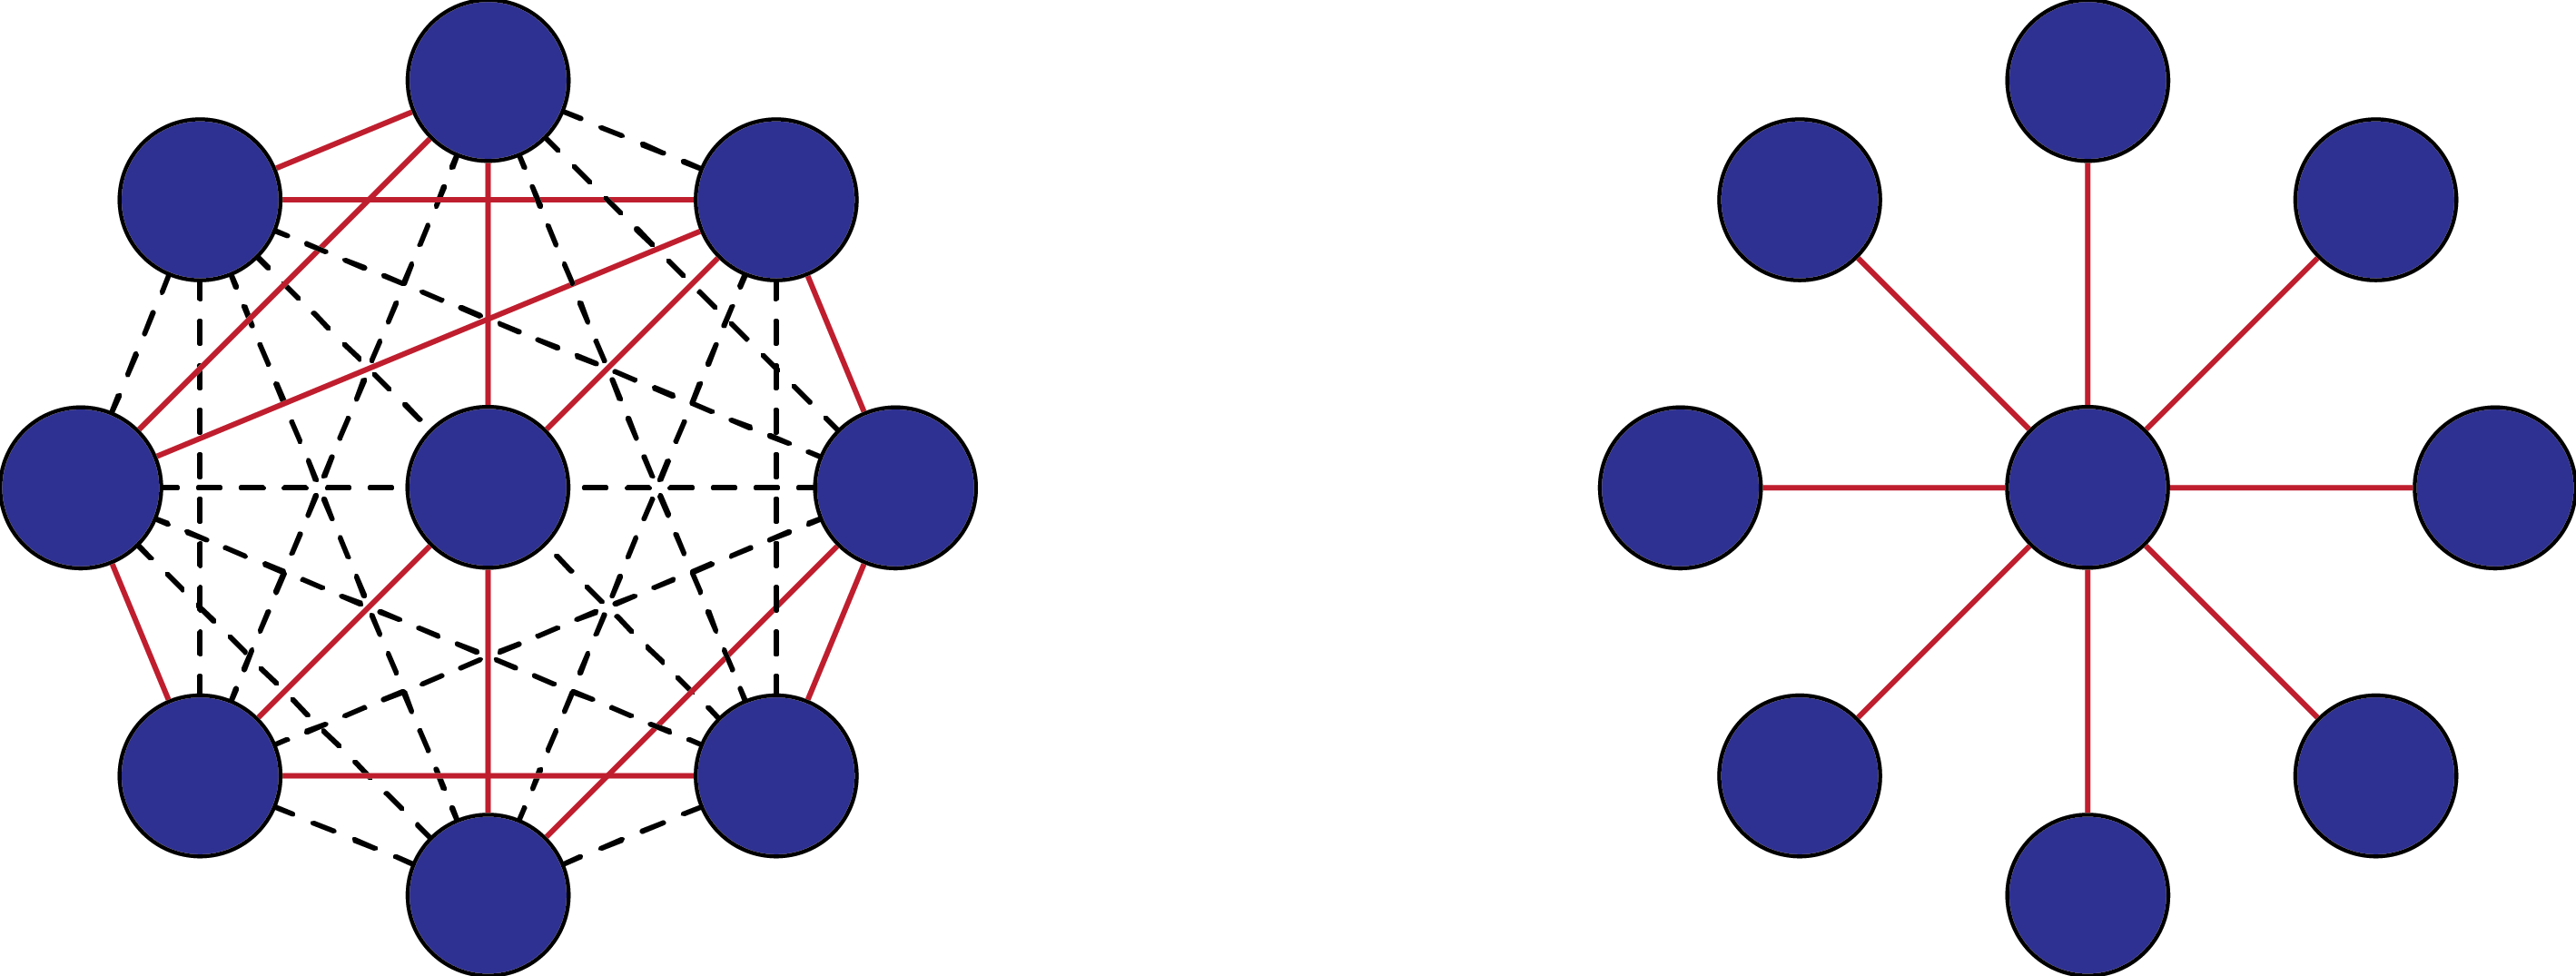
\includegraphics[width=0.6\columnwidth]{images/mesh_vs_hub_spoke.png}
    \caption{Left: A mesh network topology, Right: A hub-spoke network topology}
    \label{fig:hub_spoke_mesh_diff}
\end{figure}

While a hub-spoke topology is sufficient for typical applications, certain use cases, especially at the "internet edge" \cite{howardCoracleEvaluatingConsensus2015} requires the resilience a mesh network provides. In the case of group robotics, "centralized systems ... require a lot of computer performance from the commander" \cite{manet_drone_semenova2015network}. On the other hand, a mesh topology is "less prone to failure" \cite{manet_drone_semenova2015network} and allows for greater independence of each node. Similarly, vehicular networks require the consideration of a "highly dynamic topology" \cite{iov_wu2016internet} where nodes are moving at high speeds but also have "high-reliability requirements" \cite{iov_wu2016internet} due to safety concerns, making mesh topologies the sensible networking topology. 


%%%%%%%%%%%%%%%%%%%%%%%%%%%%% Why consensus algorithms %%%%%%%%%%%%%%%%%%%%%%%%%%%%
% resilience and dynamic topology emphasis

However, in order to meaningfully complete a task, these groups of autonomous devices must be able to coordinate and come to an agreement or a consensus. The topic of consensus is a challenging problem in distributed systems aimed at arriving at a collective agreement across all the nodes in a system, even in the presence of malfunctioning nodes \cite{Bach_Mihaljevic_Zagar_2018}. The \textit{Byzantine Generals Problem} proposed by \textit{L. Lamport} in 1982 is an analogy that aids in visualizing the need for such algorithms \cite{Lamport_1983}. According to the \textit{Byzantine Generals Problem}, a Byzantine army wants to attack a fort. Hence, each Byzantine general must decide whether to attack the target fort or retreat for protection. The caveat is that all of the generals must perform the same action simultaneously in order to minimize the number of losses. However, the generals are located at a far distance from each other and can only communicate through designated messengers, who may be lost or captured during their mission. Thus, the generals need to find a reliable way to exchange messages and reach a consensus in order to be successful. 

Consensus algorithms ensure that the critical information is reliably replicated for each node (or "generals" in the \textit{Byzantine Generals Problem}) within a system \cite{tsitsiklis1984problems}. Consensus algorithms also ensure that the nodes within the system can work as a team and succeed in their mission even if some of the nodes fail and the network topology changes \cite{raft_paper}. Therefore, consensus algorithms play a crucial role in managing a group of nodes autonomously and provide resilience against external threats \cite{Kar_Moura_2010}. Additionally, consensus algorithms provide the flexibility to add new nodes to the network, as needed, since nodes with the network can rearrange themselves autonomously \cite{Olfati_Saber_Fax_Murray_2007}. 

Similar to the \textit{Byzantine Generals Problem}, in today's world, interconnected embedded and IoT devices often need to reach a consensus in order to perform required tasks successfully and efficiently \cite{Orostica_Nunez_2019}. For example, a group of drones tasked to survey a specific area could be pre-programmed individually to complete the task. However, in such a scenario, the communication topology may be varying due to vehicle motion and communication dropouts \cite{moreau2004stability} \cite{munoz2017adaptive}. Therefore, having connectivity and consensus between these drones could drastically increase their efficiency and success rate by dynamically updating their routes based on the new information available \cite{ren2007information}. In the event of a drone loss, the remaining drones could communicate this information, and a specific drone could take over additional tasks. Furthermore, new drones could easily be added to the group as needed since the cluster can rearrange itself with the help of the consensus algorithm \cite{chen2020achieving}.


%%%%% Combining consensus algorithms and mesh networking and embedded devices %%%%% 
% Challenge of addressing problem


\begin{figure}[H]
    \centering
    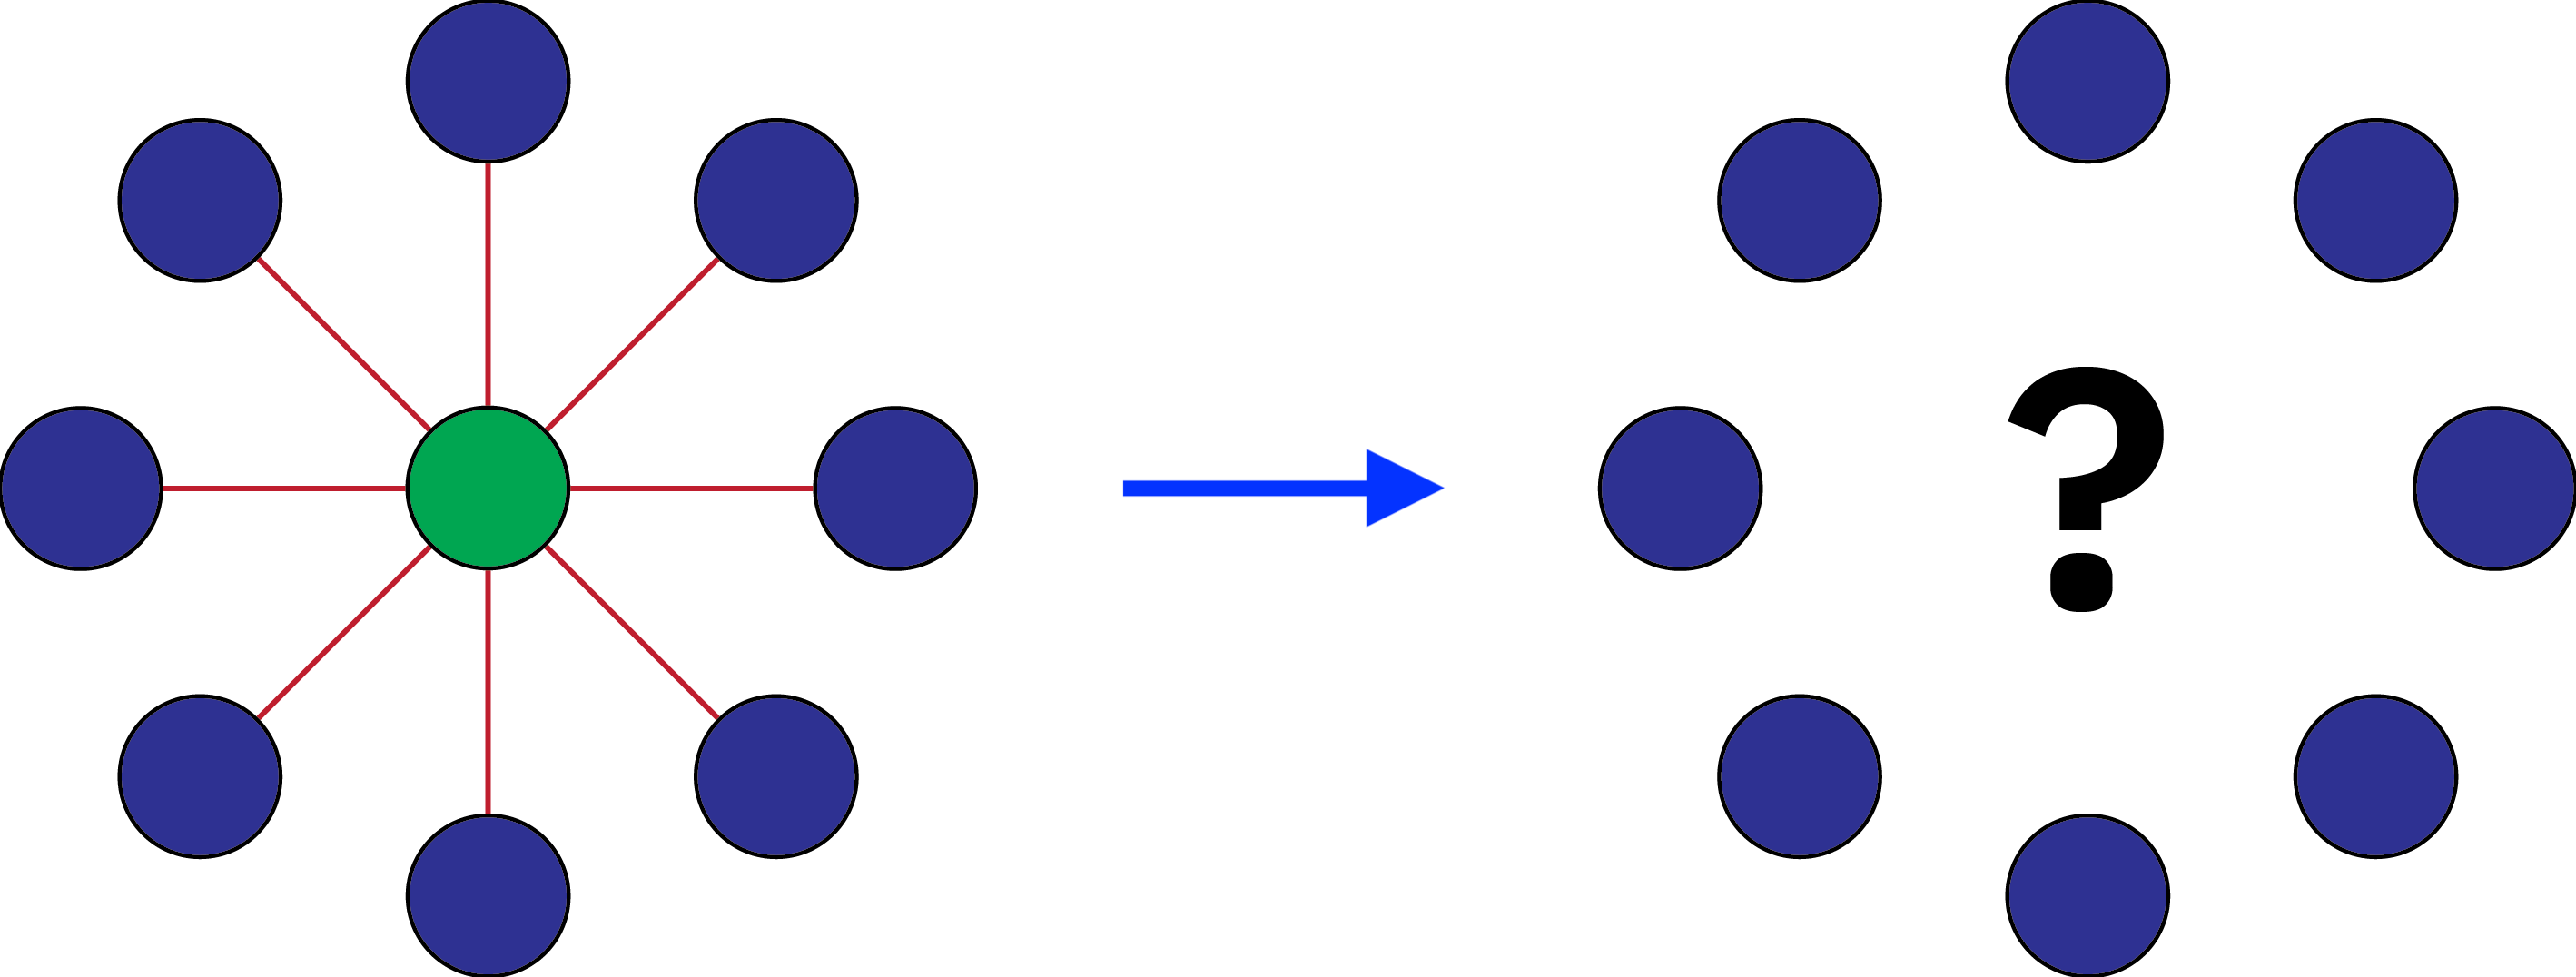
\includegraphics[width=0.6\columnwidth]{images/consensus_traditional.png}
    \caption{A consensus algorithm implemented on top of a hub-spoke network topology}
    \label{fig:consensus_traditional}
\end{figure}

A consensus algorithm could be implemented on top of traditional hub-spoke network topology, as shown in Figure \ref{fig:consensus_traditional}. The blue circles in the diagram represent the member nodes within the system, and the green circle represents the leader node. Since a hub-spoke topology is used, the green circle also represents the "hub" node in the network topology, where all of the connections meet and redistribute. A consensus algorithm implemented in this way would work without issues until there are failures stemming from the leader node. Even though consensus algorithms are capable of electing new leaders \cite{raft_paper}, the consensus algorithm would fail when the "hub" node fails in a hub-spoke network topology. This is the case because the member nodes in the system would not be able to communicate with each other to perform the election of a new leader or share information. Therefore, consensus algorithms implemented on a hub-spoke network topology are prone to a single point of failure \cite{karatas2020multi}. Given the previous drone example, if the "hub" drone fails during the mission, the rest of the cluster would not be able to communicate with each other and arrive at a consensus \cite{ren2007information}.

\begin{figure}[H]
    \centering
    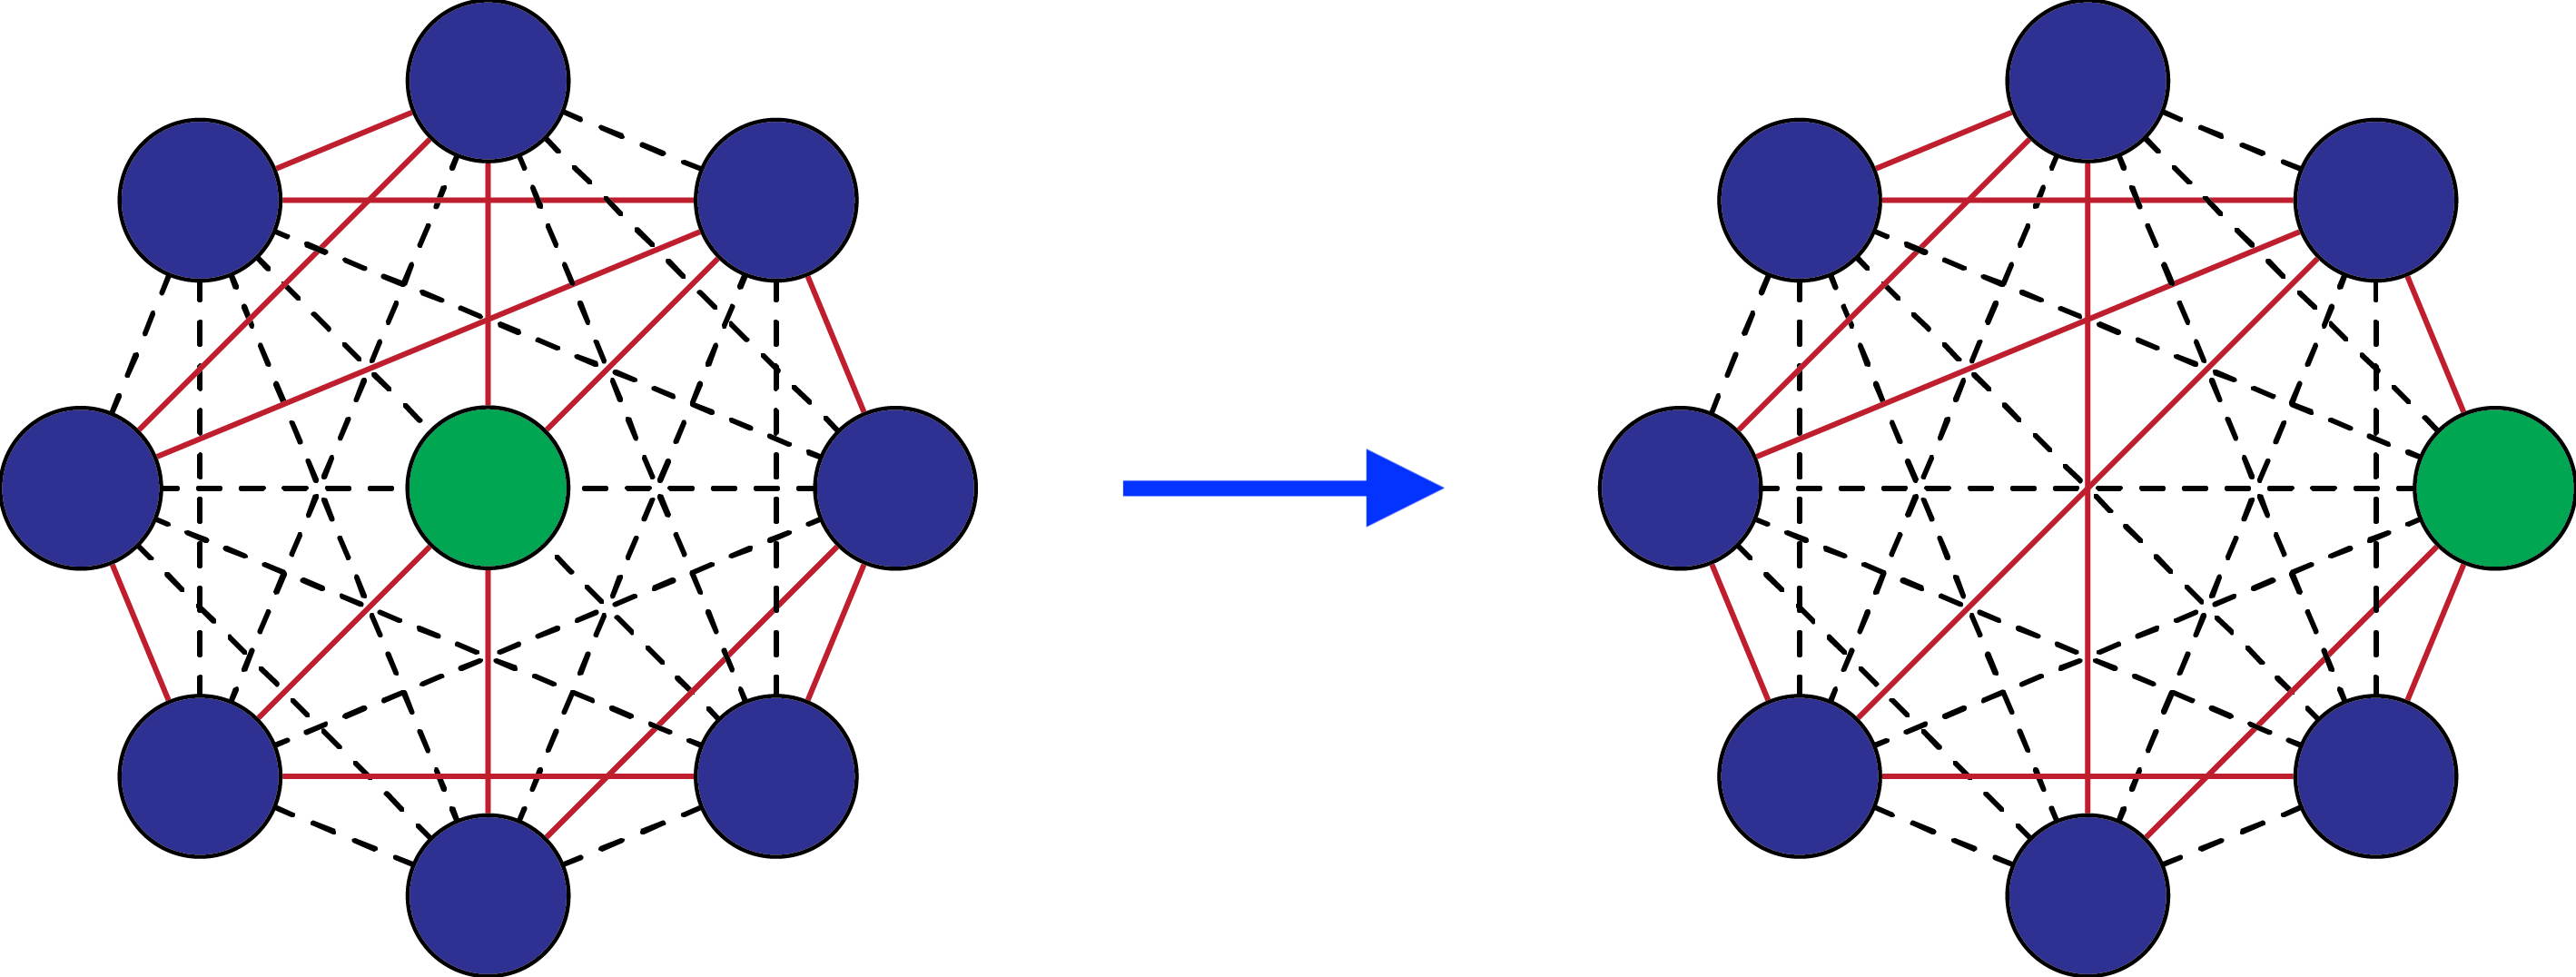
\includegraphics[width=0.6\columnwidth]{images/consensus_mesh.png}
    \caption{A consensus algorithm implemented on top of a mesh network topology}
    \label{fig:consensus_mesh}
\end{figure}

Consensus algorithms can also be implemented on top of a mesh network topology, as shown in Figure \ref{fig:consensus_mesh}. Once again, the blue circles represent the member nodes, while the green circle represents the leader node. As opposed to the implementation shown in Figure \ref{fig:consensus_traditional}, every member code can connect to each other without the need for a "hub" node. Thus, even if the leader node fails, the remaining nodes can elect a new leader node and reach a consensus. There is no single point of failure in the system shown in Figure \ref{fig:consensus_mesh}, and this situation significantly increases a system's resilience and flexibility. In light of these insights, our capstone project aims to combine mesh networking with consensus algorithms.

%%%%%%% PROBLEM DEFINITION %%%%%%%
\newpage
\section{Problem Definition}
\subsection{Problem Analysis}
In order to clarify the scope of the problem, the following questions were considered:

\begin{enumerate}

    \item Who has the problem?
    \begin{itemize}
        \item Researchers and developers who are working with clusters of mobile machines (drones, cars, rovers, etc.) operating at the internet edge with embedded systems that are tasked to achieve a mission autonomously.
    \end{itemize}
    
    \item What is the problem?
    \begin{itemize}
        \item In certain cases, these autonomous devices may fail to complete a mission or a set of tasks due to communication issues amongst themselves when using a hub-spoke system. There is no flexible and open-source software library to remedy this.
    \end{itemize}
    
    \item Where does the problem occur?
    \begin{itemize}
        \item The problem can occur in geographies where stable communication between devices connection is not possible or where the devices are not easily accessible to service by humans.
    \end{itemize}
    
    \item When does the problem occur?
    \begin{itemize}
        \item The problem can occur at any moment since it may be a result of the leader or a hub node failing within a hub-spoke topology.
    \end{itemize}
    
    \item Why does the problem occur?
    \begin{itemize}
        \item The problem occurs because all traffic is routed through these leader or hub nodes. If this node fails, communication also fails because other nodes are not able to organize themselves. The existing solutions are consensus algorithms modified by researchers but unavailable for easy deployment to the wider population.
    \end{itemize}
\end{enumerate}

We also derive further questions from the analysis above:

\begin{enumerate}

    \item What has the typical focus been on addressing the problem?
    \begin{itemize}
        \item In our background research, we have determined that most researchers attempt to develop modified consensus algorithms to better fit the mesh network; however, these modified frameworks are often only discussed in theory, and the implementation is never published in an easy to deploy format.
    \end{itemize}
    
    \item How do we address the issue of developing a ubiquitous solution accessible to multiple hardware devices?
    \begin{itemize}
        \item While the scope of the deliverables in this project may be limited to specific hardware, we can attempt to develop a community around the idea to encourage contributions from other researchers. To this effect, we can also select a popular piece of hardware to allow for more testers and wider outreach.
    \end{itemize}
\end{enumerate}



\subsection{Problem Clarification}
%   Problem Clarification
    % Black-box model
%%%%%%% %%%%%%% %%%%%%% 

Autonomous devices with embedded systems and limited power and computational resources can benefit from consensus algorithms for coordination tasks. However, such an implementation is not yet openly available. To address this, in this section, we attempt to explore the system and the sub-problems it implies.

\begin{figure}[H]
    \centering
    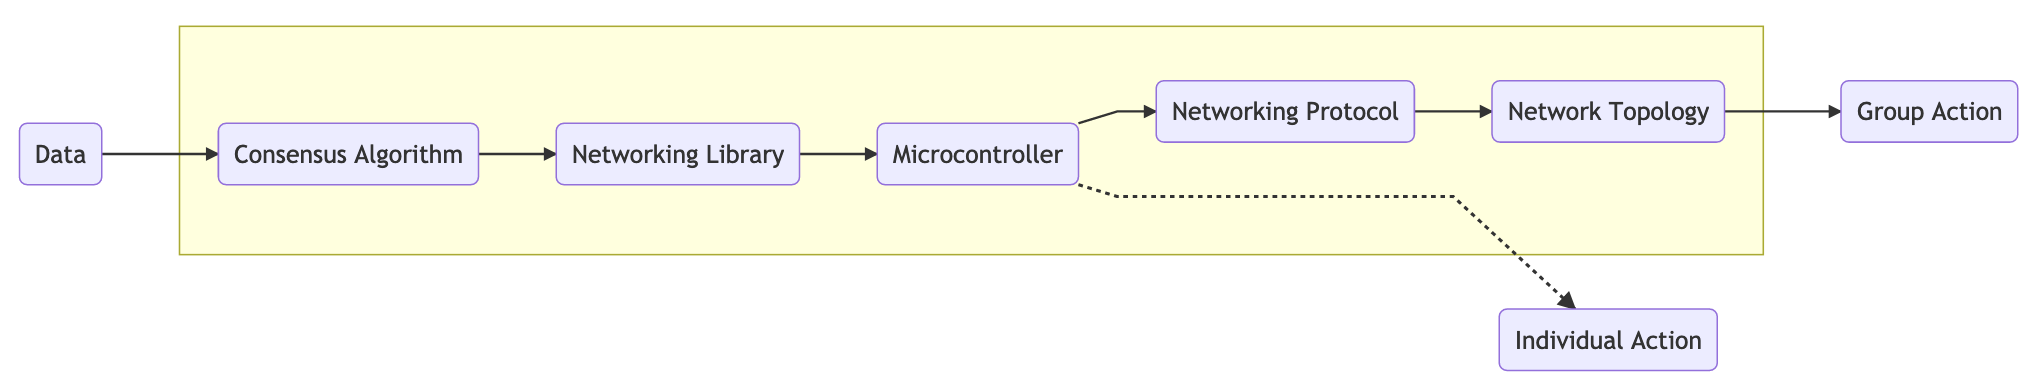
\includegraphics[width=0.90\columnwidth]{images/blackbox.png}
    \caption{A black box diagram for each node of the system}
    \label{fig:black_box}
% graph LR
%   cons(Consensus Algorithm)
%   netProc(Networking Protocol)
%   netTop(Network Topology)
%   netLib(Networking Library)
%   cont(Microcontroller)
%   data(Data)
%   groupaction(Group Action)
%   localaction(Individual Action)

%   data --> cons
%   subgraph " "
%     cons --> netLib --> cont --> netProc --> netTop
%   end
%   netTop --> groupaction
%   cont -..-> localaction
\end{figure}

The black-box model of a node in the described system, broken into its sub-problems, is shown in Figure \ref{fig:black_box}. Each of these sub-problems is further discussed in the following sub-sections. A more detailed black-box model encompassing these details can be seen in Figure \ref{fig:final_design_node_bb}. 

The sensors on a node will be collecting data, which will then be fed into the decision logic, implemented as a consensus algorithm. Each of these nodes will be communicating with one another using a Wi-Fi-based mesh network and updating their logs as a result of this communication. Eventually, each of the nodes will then carry out some actuation or state indication.

As there are multiple implementations of an 802.11 based mesh network, it is out of the scope of this project to be able to interface with all of them. Our implementation will focus on what is readily available and will be designed in a way so that with minimal future development, another implementation of a mesh network could replace the one we use.

There are also quite a few options for consensus algorithms. However, our system will be limited to a single consensus algorithm, namely Raft \cite{raft_paper}. Section \ref{conceptualization_consensus} describes the reasoning behind selecting Raft.


\subsubsection{Network Topology}
\label{section:network_topology}
We conduct a detailed analysis of network topologies in Section \ref{section:background_research}. Figure \ref{fig:hub_spoke_mesh_diff} outlines two possible network topologies: mesh and hub-spoke.

\subsubsection{Networking Protocols}
\label{section:networking_protocols}
There are a plethora of network types for wireless communication, often dependent on the application of the system. From literature, we identify four dominant protocols: Bluetooth, Ultra-wideband (UWB), Zigbee, LoRa, and Wifi \cite{lee2007comparative, ti_lethaby2017wireless}.

Mesh networks are not limited to any one of these standards. In fact, "IoT-related wireless technologies ... are extremely heterogeneous in terms of protocols, performance, reliability, latency, cost-effectiveness, and coverage",  \cite{iot_survey_cilfone2019wireless}. Each standard has its niche of operation: IoT devices may employ the IEEE 802.15.4 standard or Bluetooth for short-range communications, whereas mid to long-range communications may make use of IEEE 802.11, which was amended in 2011 to support mesh networks \cite{ti_lethaby2017wireless, iot_survey_cilfone2019wireless}. Figure \ref{fig:comparison_protocols} shows a comparative performance analysis of LoRa, Zigbee, WiFi, and Bluetooth, highlighting how each protocol has its strengths and weaknesses.


\begin{figure}[H]
    \centering
    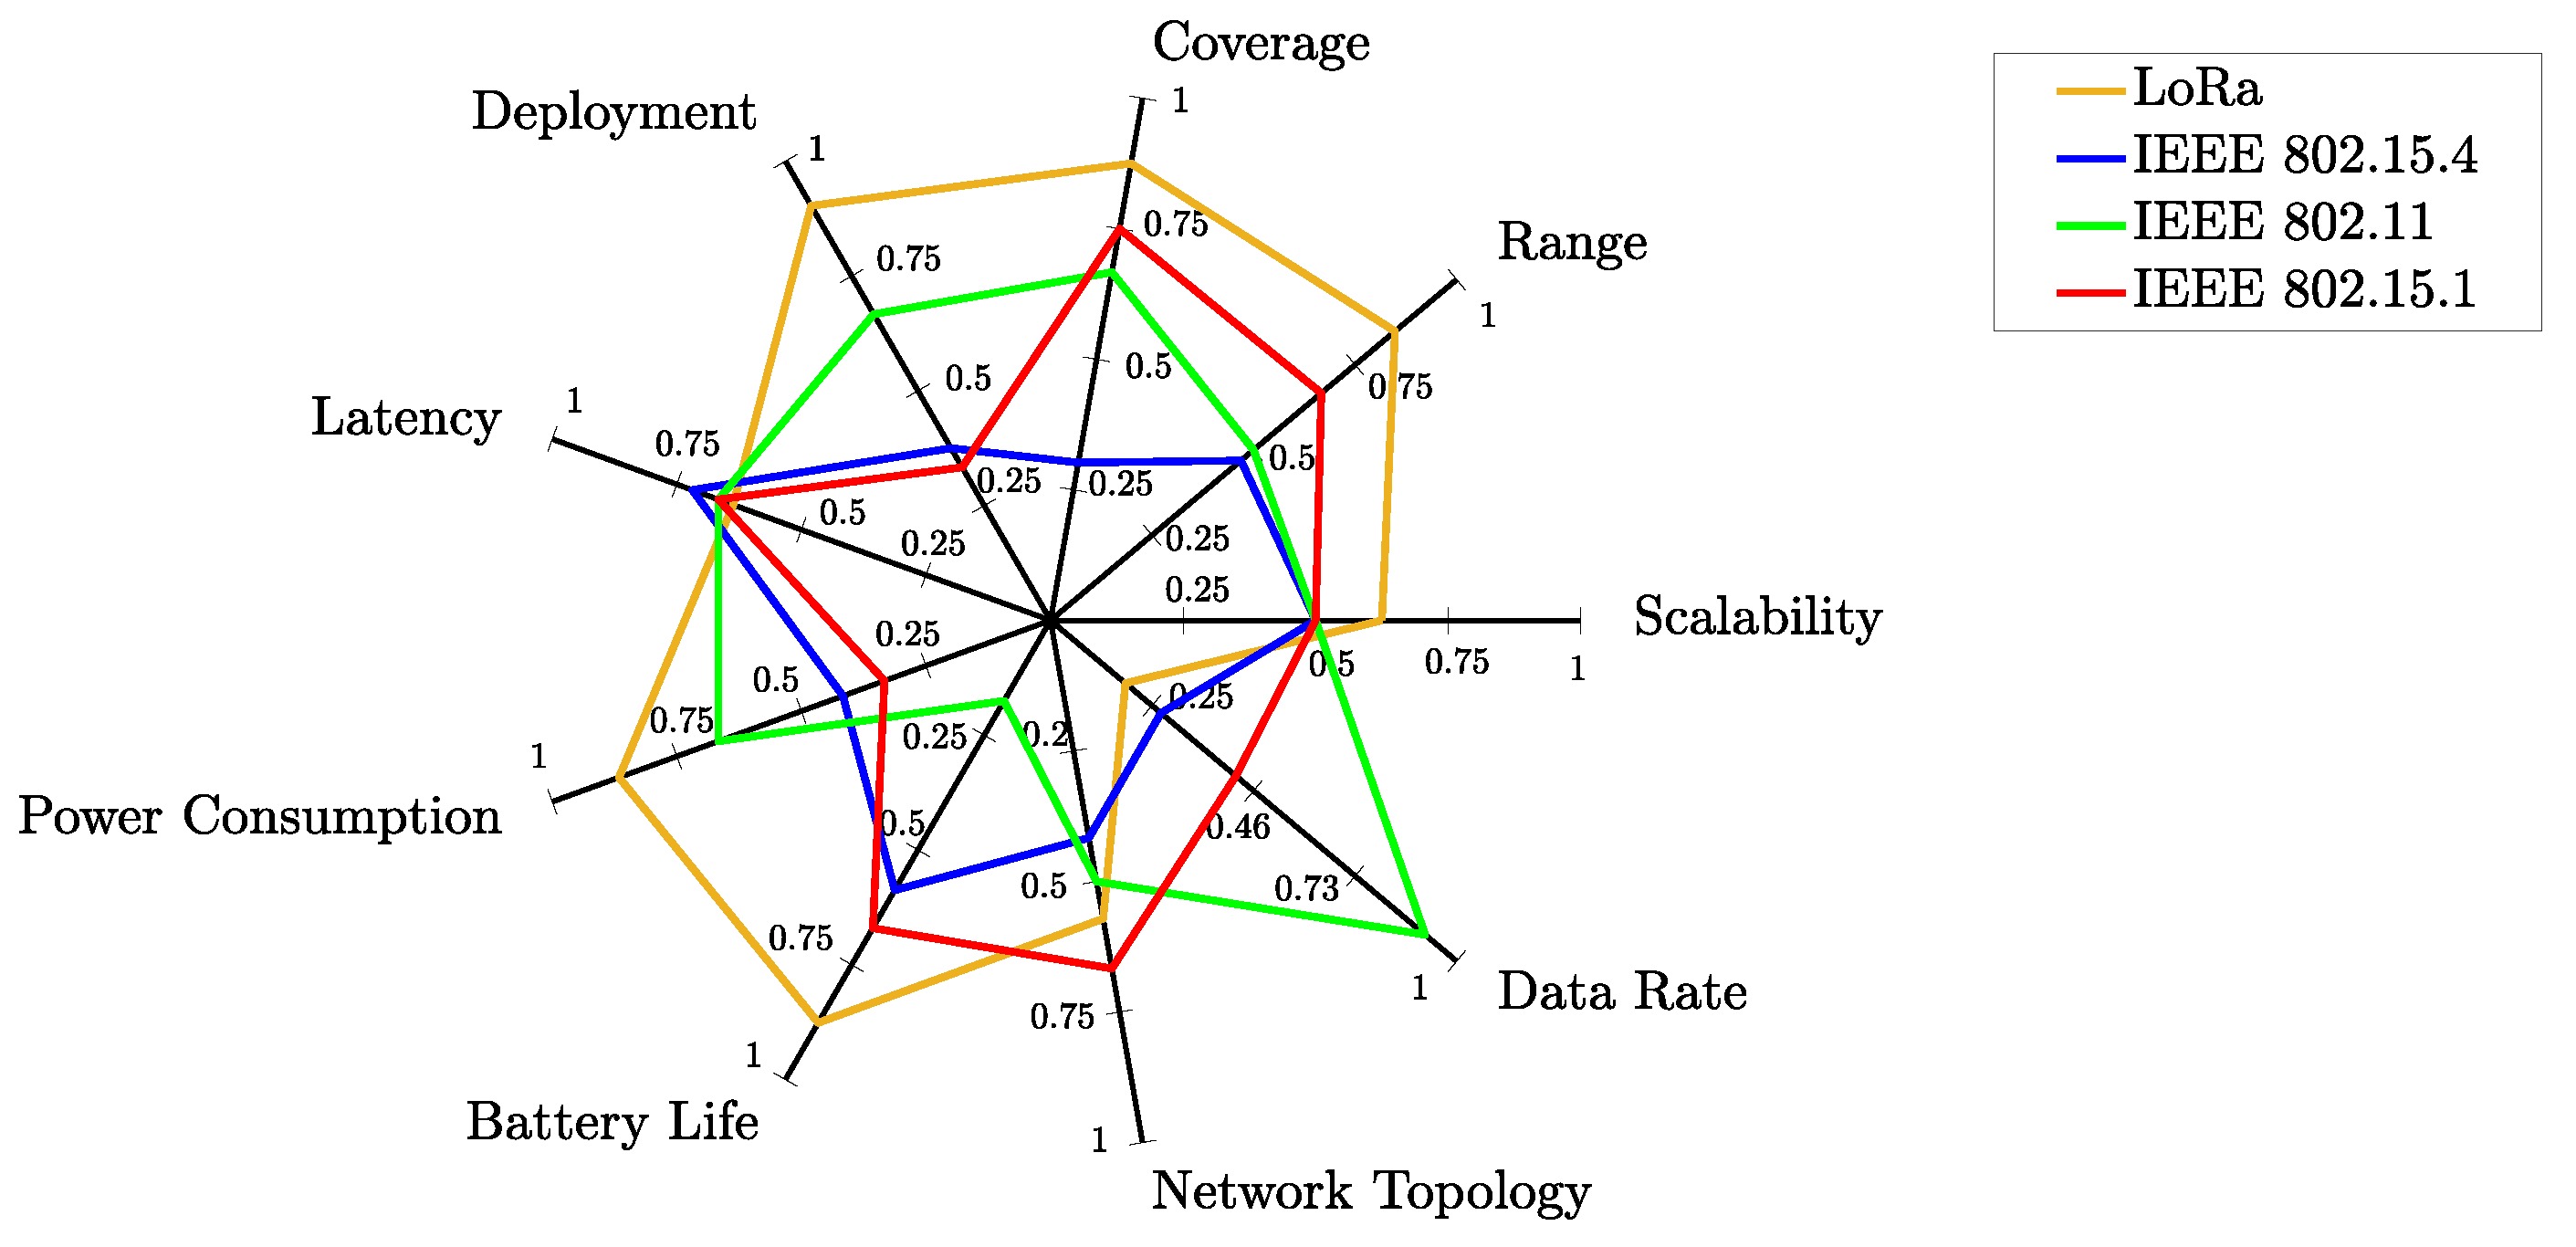
\includegraphics[width=0.8\columnwidth]{images/comp_perf_analysis.png}
    \caption{Comparative performance analysis of four protocols. \\ Adapted from \cite{iot_survey_cilfone2019wireless}}
    \label{fig:comparison_protocols}
\end{figure}


While the implementation of mesh networks and consensus algorithms are agnostic to the protocol underneath, it is important to address these concepts in the context of real-world constraints. Current IoT research "assumes that the devices are equipped with low-power IEEE 802.15.4 (Zigbee) transceivers" \cite{disney_glaropoulos2013enhanced}. Yet, a significant portion of deployed embedded systems and consumer electronics carry IEEE 802.11 compatible hardware \cite{disney_glaropoulos2013enhanced}. 
The "wide penetration of IEEE 802.11" \cite{disney_glaropoulos2013enhanced} then makes it the more attractive choice because the hardware does not need to be redeployed to support newer standards. Despite 802.11's notoriety as high power consumption, research indicates that additional firmware controlling the sleep schedule can help lead to significant energy savings \cite{disney_glaropoulos2013enhanced, barghi2019practicalpower}.

Furthermore, 802.11 has built-in support for mesh networks as a result of the 802.11s amendment. The amendment describes mesh stations (mesh STAs) and their ability to link with one another without the requirement of a central AP; rather, certain nodes may act as mesh access points (MAP) to connect to another network \cite{iov_wu2016internet, optical_zeitgeist_laboratory_2011}.

Given 802.11's ubiquity and built-in support for mesh networks, we found it fit to work with an 802.11-based network.

\subsubsection{Consensus Algorithms}
\label{conceptualization_consensus}
With the rapid increase in adoption and development of distributed \& multi-agent systems, achieving a consensus across these systems became an important issue because of the high potential for scalability \cite{Ge_Han_Ding_Zhang_Ning_2018}. Achieving consensus across such systems allows autonomous air vehicles, cooperative IoT devices, sensor networks to be built at a scale. 

The distributed consensus algorithms can be classified into three categories based on their hierarchical structure: \emph{leaderless consensus algorithms}, \emph{leader-following consensus algorithms}, and \emph{containment control algorithms} \cite{consensus_systems_survey}. In \emph{leaderless consensus algorithms}, there are no leaders, and the nodes within the system are expected to asynchronously converge on a target \cite{Ge_Han_2017}. However, in \emph{leader-following consensus algorithms}, there is a leader node that orchestrates the actions of the rest of the network. Finally, in \emph{containment control algorithms}, there might be more than one leader to orchestrate different types of operations within the system. A visualization of the different types of consensus algorithms can be seen in Figure \ref{fig:consensus_types_detailed}, where green circles are the leaders in the system, and orange lines represent the logical connections between the consensus members.


\begin{figure}[H]
    \centering
    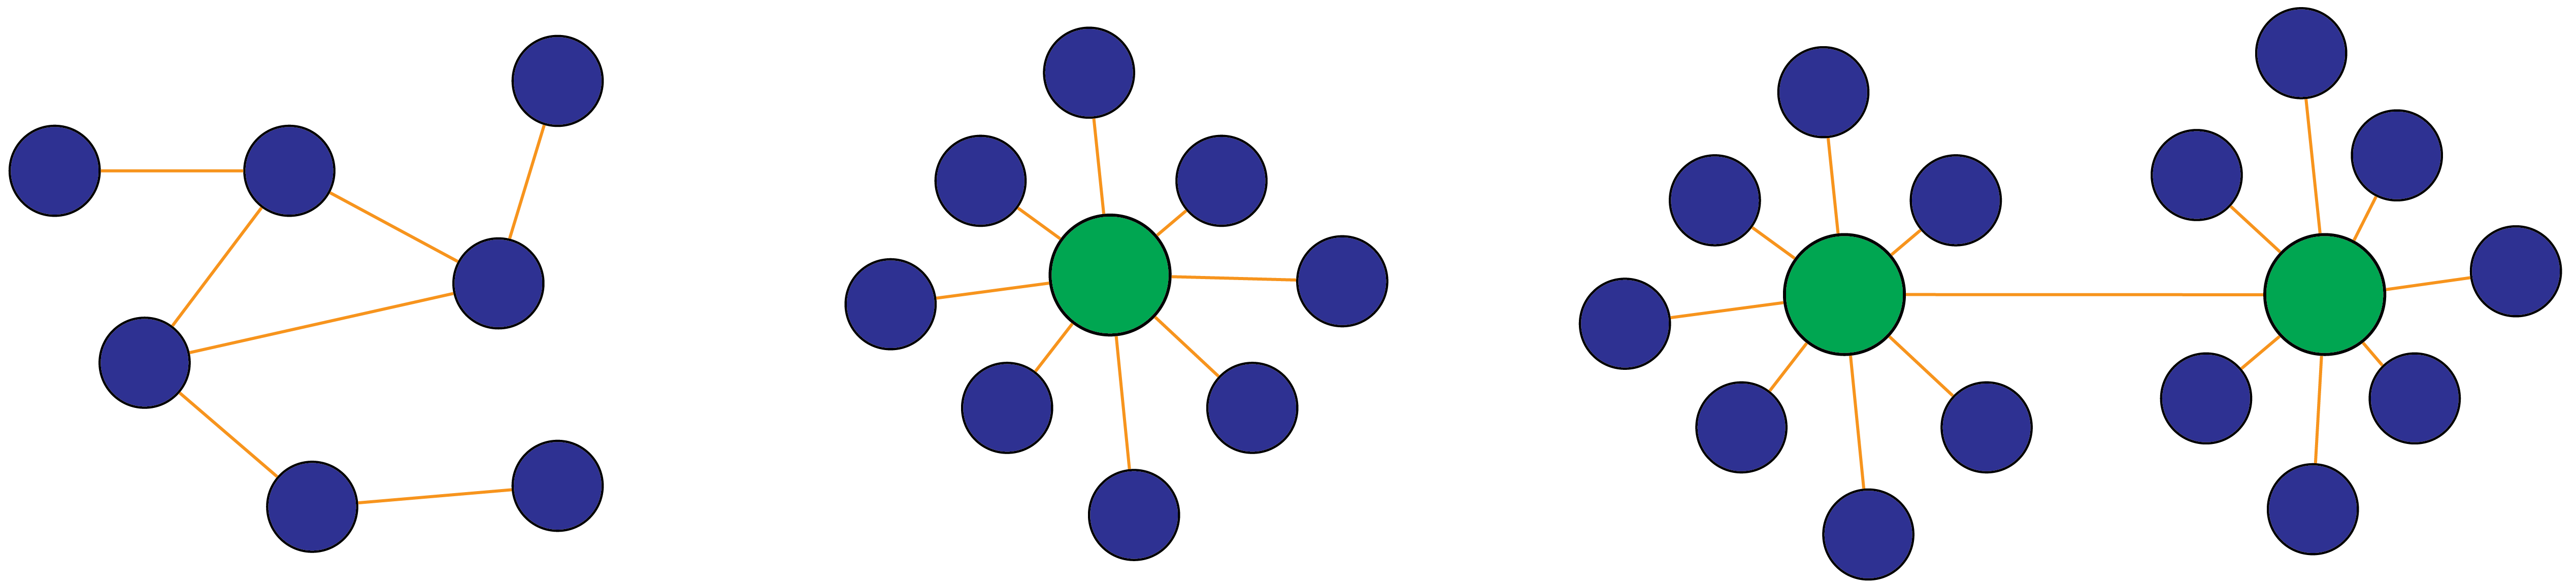
\includegraphics[width=0.99\columnwidth]{images/consensus_types.png}
    \caption{Left: A leaderless consensus algorithm, Middle: A leader-following consensus algorithm, Right: A containment control algorithm}
    \label{fig:consensus_types_detailed}
\end{figure}


The distributed consensus algorithms can also be classified into two categories based on when they transfer information to reach a consensus: \emph{time-triggered consensus algorithms} and \emph{event-triggered consensus algorithms} \cite{consensus_systems_survey}. In \emph{time-triggered consensus algorithms}, the nodes in the system initiate the information transfer once a set amount of time elapses. Additionally, if the consensus algorithm is asynchronous by design, each node can have a randomly set time duration before they send information. On the other hand, in \emph{event-triggered consensus algorithms}, the nodes in the system initiate information transfer when an external event occurs. A visualization of the different types of consensus algorithms can be seen in Figure \ref{fig:consensus_time_based_and_evevent_based}, where orange circles represent the timer of the nodes, the green arrow represents the external event trigger, and red arrows represent the information transfer.

\begin{figure}[H]
    \centering
    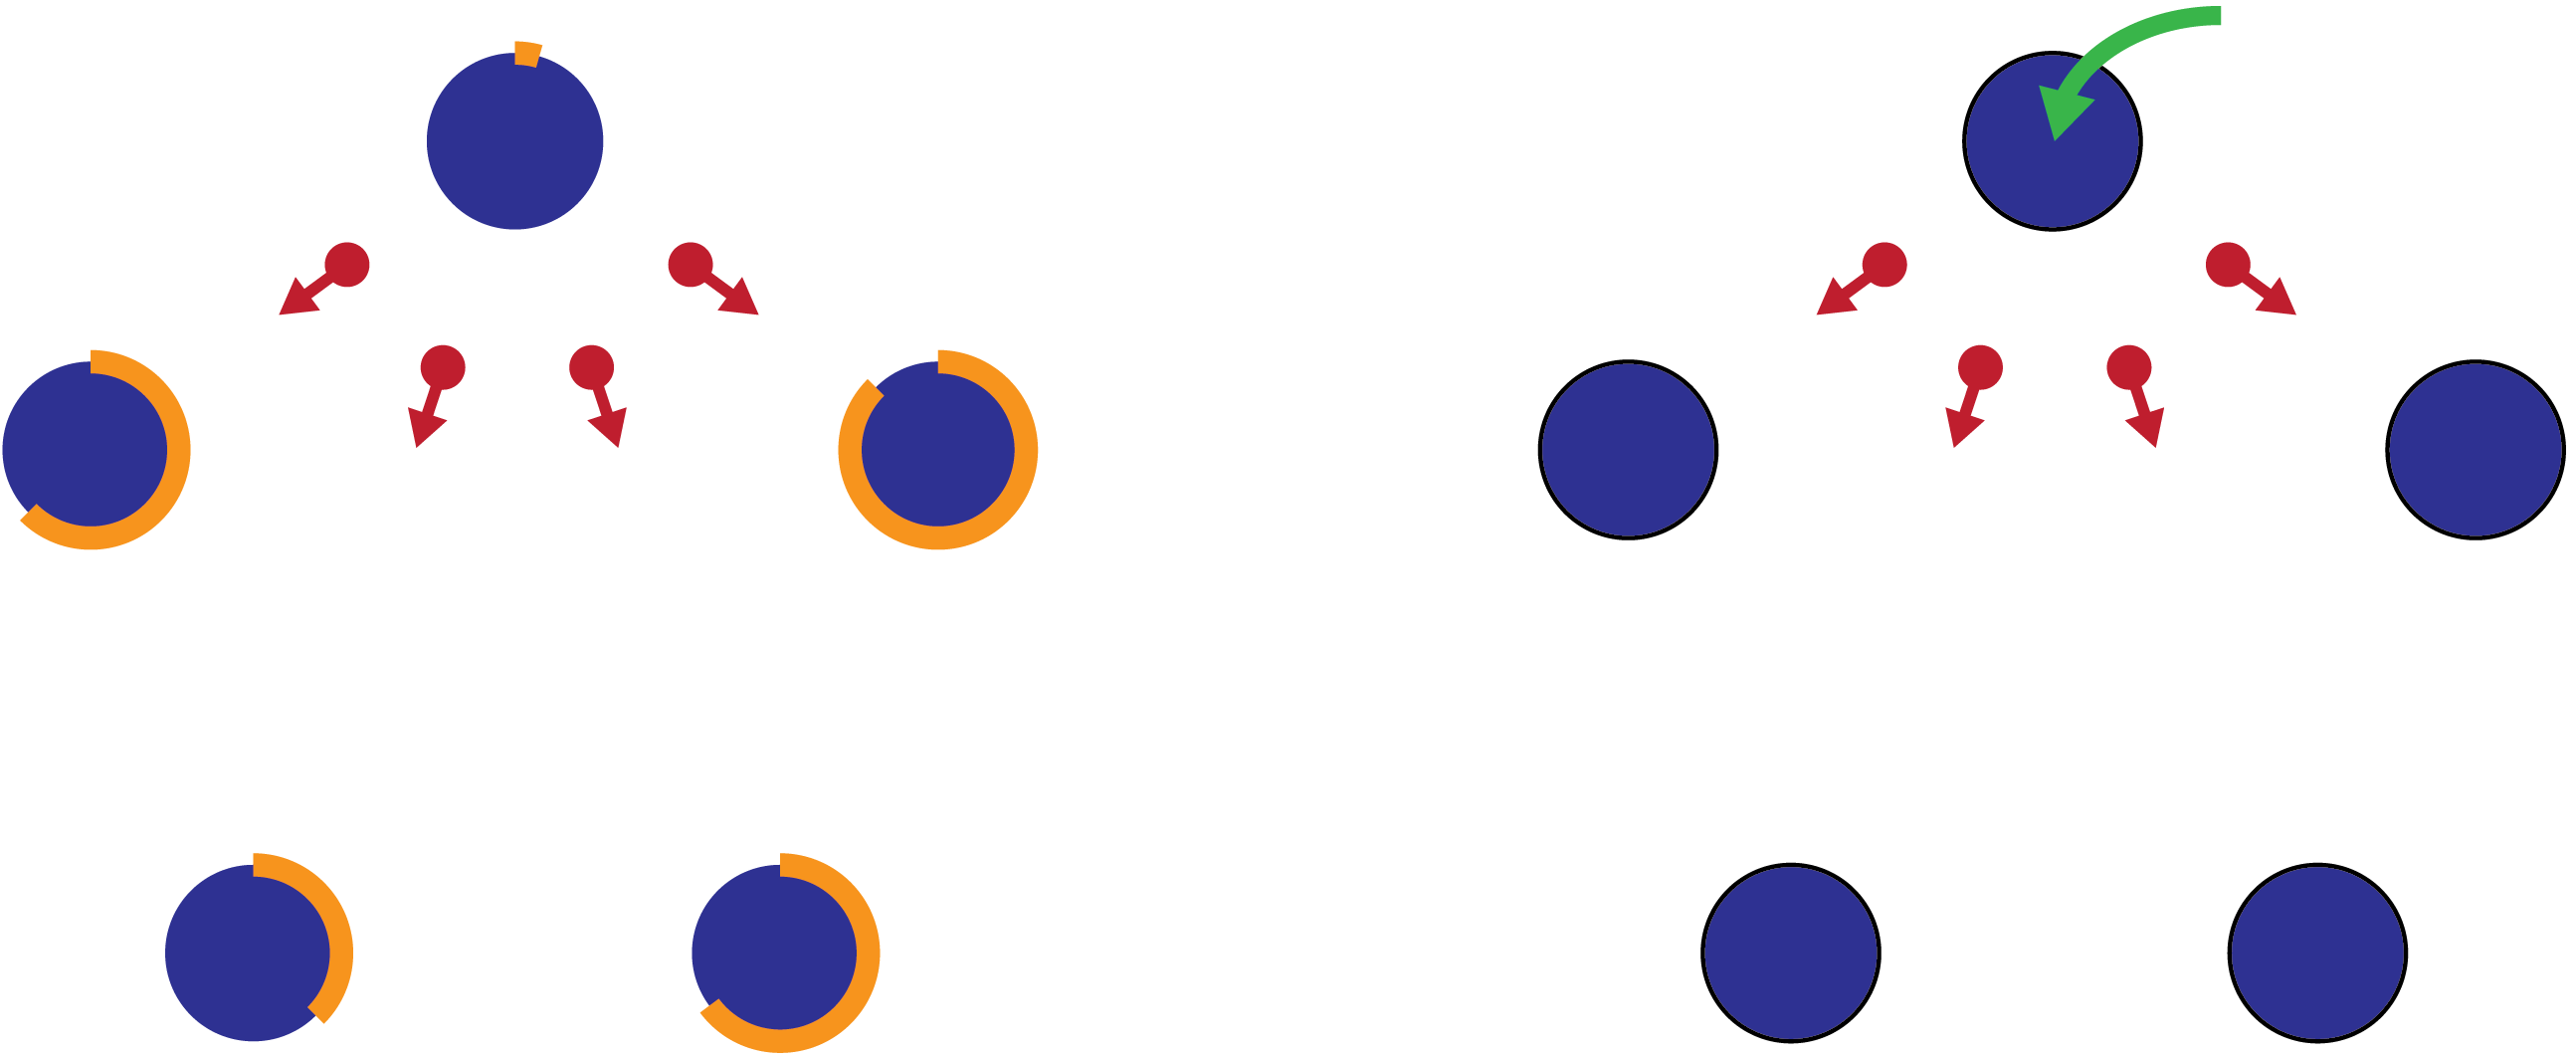
\includegraphics[width=0.55\columnwidth]{images/consensus_time_based_and_evevent_based.png}
    \caption{Left: A time-triggered consensus algorithm exchanging messages when the timer goes off, Right: An event-triggered consensus algorithm exchanging messages when an event occurs (green arrow)}
    \label{fig:consensus_time_based_and_evevent_based}
\end{figure}

Paxos and Raft are among the most popular \& practical distributed \emph{time-triggered} and \emph{leader-following} consensus algorithms available \cite{paxos_vs_raft}. Paxos has been the industry standard since it was first published, despite its status as a difficult to understand and implement as an algorithm. Since the Raft consensus algorithm aims to be simple and easy to understand \cite{raft_paper}, it is gaining popularity in the industry. Furthermore, the Raft consensus algorithm aims to abstract away how the underlying technology works and avoid a system-specific implementation \cite{paxos_vs_raft}. As a result, the Raft consensus algorithm is more suitable for experimenting and implementing non-traditional topologies like mesh networks.

\subsubsection{Microcontrollers}
Microcontroller units (MCUs) are a hefty consideration for any IoT solution. Unsurprisingly, there is a large variety of MCUs at different levels of "memory, power, computational capability, architecture etc." \cite{bansal2020iotsurveydevices} for various applications. These devices sit at different levels of the IoT ecosystem, implying that not all devices are required to be homogeneous in their capabilities. For discussion purposes, we adopt the classification system described in Bansal & Kumar's survey of IoT technologies \cite{bansal2020iotsurveydevices}. Class 0 devices may have 1-50KB of RAM with clock speeds below 100MHz, class 1 devices range from 100KB-100MB of RAM with clock speeds between 100MHz-1.5Ghz, and class 2 devices generally have resources greater than those of class 1 \cite{bansal2020iotsurveydevices}. Typically, class 0 devices such as the TELOSB are employed for Wireless Sensor Network (WSN) use-cases to collect data and perhaps perform simple actuation. On the other hand, class 1 devices, such as the well-known Raspberry Pis, are more suitable for coordination, media processing, data filtering tasks, etc.

Given our design constraints, namely dynamic topology, and decision-making capabilities, we would expect this system to work with embedded systems on mobile technologies such as drones, vehicles, and rovers. While such devices are often fitted with class 2 devices, the goal of our project is to be able to deploy such a networking ability on class 1 devices as well. Espressif's ESP8266 chip stands out as an option: the chip is designed to be a WiFi chip with a focus on low-cost and minimal peripherals. The MCU operates between 80-160MHz and has 50KB of SRAM with up to 16MB of external flash memory \cite{espressif:esp8266}, so it is on the lower end of the class 1 category. Moreover, there is a decent open-source community dedicated to the MCU, and Espressif has released a mesh networking software development kit (SDK) for its chips with detailed documentation \cite{esp-mesh-docs}. 

\subsubsection{Networking Library}
Networking libraries function as an abstraction layer for software projects to handle communication between various devices. Networking libraries usually operate on layer-3 (network layer) or layer-2 (data link layer) of the Open Systems Interconnection model (OSI model) in order to ensure an efficient, reliable, and fast delivery of the packets sent \cite{perlman1988choosing}. Furthermore, networking libraries are often capable of forming different network topologies, such as mesh and hub-spoke, based on the user choices in order to increase resiliency \cite{riggio2008hardware}.

Since Espressif's ESP8266 chip is capable of functioning as both Station (STA) and Access Point (AP) simultaneously \cite{espressif:esp8266}, there are networking libraries such as painlessMesh, ESP8266 WiFi mesh, Arduino WiFi for creating both mesh and hub-spoke networks \cite{yoppyperformance}. Among these networking libraries, painlessMesh is one of the more practical and easy to configure options. The library forms an "ad-hoc network which requires neither routing plan nor central controller"  \cite{yoppyperformance} for the resource-limited ESP8266 boards. painlessMesh uses the boards' unique 32-bit MAC addresses \cite{painlessMesh} in order to decrease network setup overhead and distinguish each node in the network, instead of using Internet Protocol (IP) addresses. Furthermore, painlessMesh time synchronizes all nodes "with a precision of less than 10 ms," \cite{yoppyperformance} allowing for real-time synchronized voting in the Raft consensus algorithm. Finally, painlessMesh also makes use of multi-hop messages in the mesh network \cite{painlessMesh} to improve network coverage and reliability of packet delivery. 


\subsection{Problem Statement}
%   Problem Statement
    % Clarify the scope of the problem [kinda done]
    % Project Aim [done]
%%%%%%% %%%%%%% %%%%%%% 

We have identified the problem to be the lack of a flexible and easy to access software library that implements a consensus algorithm atop a mesh network for low-power embedded systems in dynamic environments.

% The objective of this Capstone Project is to design and develop a resilient wireless mesh network architecture coupled with a consensus algorithm for low-power embedded devices in dynamic topologies, demonstrated using 802.11-based ESP8266 boards.

In order to address this problem, we aim to create an open-source software library that can be incorporated into an application that requires nodes to work autonomously together. We plan to demonstrate our software library through prototype boards that will each consist of an ESP8266 MCU, power sensors, and LEDs. Our software library will be installed on these boards, enabling them to form a mesh network and run the Raft consensus algorithm. We will show how a signal propagates in the Raft consensus algorithm within the mesh network using LEDs, as shown in Figure \ref{fig:mesh_signal_propagation}. We will also demonstrate how the network can realign \& recover by turning on and off randomly selected ESP8266 microcontrollers to emulate a dynamic environment.

Furthermore, with our software library, we aim to achieve a packet delivery rate of a minimum of 95\% and an average latency smaller than 20ms between nodes on the mesh network while having a maximum leader selection time of 1000ms for the Raft consensus algorithm. The software library should also be able to accommodate at least 100 nodes in the mesh network and have a total size of 2MB when compiled with the avr-gcc compiler.

\begin{figure}[H]
    \centering
    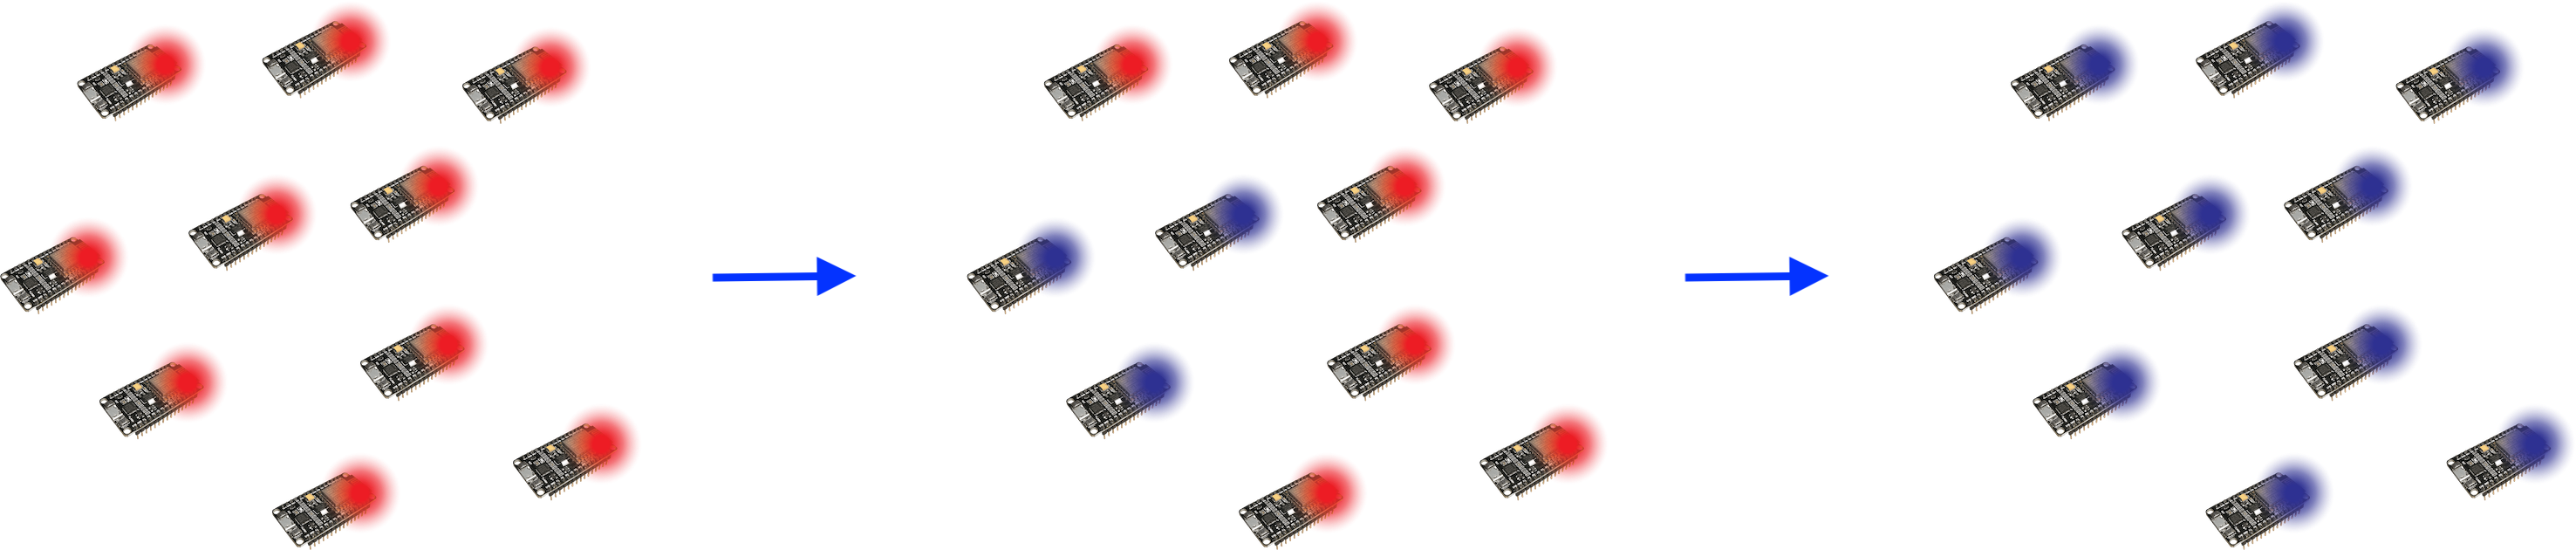
\includegraphics[width=0.8\columnwidth]{images/mesh_signal_propagation.png}
    \caption{An ESP8266 cluster transitioning to the blue state from the red state using our software library. Red and blue LEDs are used to represent the states.}
    \label{fig:mesh_signal_propagation}
\end{figure}

% giving specs and constraints in quantitative terms



\newpage
\subsection{Design Constraints}
\subsubsection{Technical}

Taking into account market demands, the history of the topic, and potential applications, there are various technical constraints on our system:

\begin{itemize}
    \item \textit{Resilient to threats:}
    \begin{itemize}
        \item  The system should also be resilient to handling abrupt changes to the system, such as the loss of a leader, ensuring that the task is truly distributed. 
        \item The final design aims to recover from the loss of a consensus leader within 1000\si{\ms}.
    \end{itemize}
    
    \item \textit{Scalability:} 
    \begin{itemize}
        \item The system should be able to perform with various densities of nodes. For example, increasing the number of nodes in a given area should not significantly increase latency. 
        \item The final design aims to support at least 100 nodes in an area covering 1000\si{m^2}.
    \end{itemize}
    
    \item \textit{Low power consumption:}
    \begin{itemize}
        \item Since this system is centered around embedded devices deployed in the real-world, the implementation should consider limitations in access to power. 
        \item The final design is aimed to be consuming below 100\si{mA} on average use.
    \end{itemize}
    
    \item \textit{Small footprint:} 
    \begin{itemize}
        \item The compiled code for the system should be small enough to fit into the memory of an embedded system. 
        \item The final design is aimed to fit into an embedded 2\si{MB} flash memory.
    \end{itemize}
\end{itemize}

\subsubsection{Non-Technical}

We also consider non-technical constraints:

\begin{itemize}
    \item \textit{Modular design:} 
    \begin{itemize}
        \item  Although the implementation in this project is for an IEEE 802.11 based chip, the system should be designed so that it may be ported to another underlying protocol.
    \end{itemize}
    
    % \item \textit{Decision making:} 
    % \begin{itemize}
    %     \item  The system should be capable of coordinating all of the nodes to successfully arrive at decisions, ensuring that the consensus algorithm is meaningfully implemented.
    % \end{itemize}
    
    \item \textit{Dynamic topology:}
    \begin{itemize}
        \item  The system should be capable of performing on mobile technologies, where nodes are constantly entering and exiting the network.
        %, potentially at high speeds.
    \end{itemize}
    
    \item \textit{Versatility:}
    \begin{itemize}
        \item  Given that neither consensus algorithms nor mesh topologies are concepts with limited applications, the system should maintain this quality and ideally be able to operate on various technologies such as UAVs, cars, rovers, etc.
    \end{itemize}
    
    \item \textit{Open-Source:}
    \begin{itemize}
        \item  This project should be built with the potential to have a community develop around it for future development, implying a permissible license, proper documentation, and ease of access. The system should not be limited to expensive and obscure technology.
    \end{itemize}
\end{itemize}
 



%%%%%%% CONCEPTUALIZATION %%%%%%%
\newpage
\section{Conceptualization}
\subsection{Concept Generation}

Following the black box model in Figure \ref{fig:black_box}, we generated the concepts in the morphological chart shown in Table \ref{tab:morph_chart}.

\begin{itemize}
	\item \textbf{Networking Protocol} - While we will design our system to be modular and potentially connect with any networking protocol, we must select a protocol upon which to prototype. Through a literature search, we were able to find the most commonly used networking protocols available for Internet of Things (IoT) solutions.
	\item \textbf{Networking Topology} - There are multiple topologies available to network devices. The hub-spoke topology and mesh topology are the most relevant to wireless devices.
	\item \textbf{Consensus Algorithm} - Central to our project, we have a variety of consensus algorithms to select from. We narrow our scope to look specifically at distributed consensus algorithms. 
	\item \textbf{Microcontroller} - IoT devices come in multiple different capabilities. While some are quite powerful and packed with significant resources, others are very simple systems meant for trivial tasks. The choice of IoT devices is important for performance, power consumption, and memory considerations.
	\item \textbf{Networking Library} - Networking libraries provide an API to abstract away the lower-level networking implementation. Hence, the selected library must be easy to use and allow for flexibility in implementation. 
	%\item \textbf{Battery} - For our prototype, we want to have access to mobile nodes and will thus develop our own prototype board powered by batteries so that it is not tethered to a power source.
\end{itemize}


\begin{table}[H]
    \scriptsize
    
    % Set row height
    \renewcommand{\arraystretch}{1.3}
    \vspace{10pt}
    
    \caption{Morphological chart}
    \label{tab:morph_chart}
    
    \begin{center}
        \begin{tabular}{|l|l|l|l|l|l|}
        \hline
        \multicolumn{6}{|c|}{\multirow{2}{*}{\textbf{ramen: Design and Development of a Raft Consensus Algorithm Coupled With a IEEE 802.11 Based Mesh Network for Embedded Systems}}} \\
        \multicolumn{6}{|c|}{}                                                                                   \\ \hline
        \multicolumn{1}{|c|}{Sub-Problem} & \multicolumn{5}{c|}{Available Options}                               \\        
        \thickhline
        Networking Protocol &
          IEEE 802.11 &
          IEEE 802.15.4 (Zigbee) &
          IEEE 802.15.3 (UWB) &
          802.15.1 (Bluetooth) &
          LoRaWAN \\ \hline
        Networking Topology     & Hub-Spoke Topology & Mesh Topology & Ring Topology & Bus Topology      &  \\ \hline
        Consensus Algorithm     & Paxos              & Raft          & ZAB           & Mencius           &  \\ \hline
        Microcontroller         & BCM2711            & ARM Cortex-A8 & ESP8266       & ATmega328P        &  \\ \hline
        Networking Library      & easyMesh           & painlessMesh  & ESP-MESH       & ESP8266 WiFi Mesh &  \\ \hline
        \end{tabular}
\end{center}
\end{table}
\FloatBarrier


%%%%%%%%%%%%%%%%%%%%%%%%%%%%%%%%%%%%%%%%%%%%%%%%%
\subsection{Concept Selection}

We also constructed Pugh Charts to aid in the decision-making process when evaluating alternatives compared to a baseline. Pugh Charts compare a given option to potential alternatives and compare them across various criteria. If an alternative performs better than the given option on a certain criterion, then it scores a +1. If it performs worse for the criterion, then it scores a -1; otherwise, it is assumed to perform similarly and gets a score of 0. Finally, the score across all criteria is summed to determine whether an alternative is better than the original option being considered.

\begin{table}[!h]
    \scriptsize
    
    % Set row height
    \renewcommand{\arraystretch}{1.3}
    \vspace{10pt}
    
    \caption{Pugh chart for consensus algorithm selection with Raft as base}
    \label{tab:pugh_raft}

    \begin{center}
        \begin{tabular}{@{}*{6}{|p{0.14\textwidth}|@{}}}
        \hline
        \multicolumn{1}{|c|}{Consensus Algorithm} & Ease of Access & Documentation & Relevance & Performance & Sum \\
        \thickhline
        Raft    & Base & Base & Base & Base &    \\ \hline
        Paxos   & -1   & 0    & -1   & 0    & -2 \\ \hline
        Mencius & -1   & -1   & -1   & 0    & -3 \\ \hline
        ZAB     & -1   & -1   & -1   & -1   & -4 \\ \hline
        \end{tabular}
    \end{center}
\end{table}
\FloatBarrier

\begin{table}[!h]
    \scriptsize
    
    % Set row height
    \renewcommand{\arraystretch}{1.3}
    \vspace{10pt}
    
    \caption{Pugh chart for consensus algorithm selection with Paxos as base}
    \label{tab:pugh_paxos}
    
    \begin{center}
        \begin{tabular}{@{}*{6}{|p{0.14\textwidth}|@{}}}
        \hline
        \multicolumn{1}{|c|}{Consensus Algorithm} & Ease of Access & Documentation & Relevance & Performance & Sum \\ 
        \thickhline
        Raft    & 1    & 1    & 0    & 0    & 2  \\ \hline
        Paxos   & Base & Base & Base & Base &    \\ \hline
        Mencius & 0    & -1   & -1   & 0    & -2 \\ \hline
        ZAB     & 0    & -1   & -1   & -1   & -3 \\ \hline
        \end{tabular}
    \end{center}
\end{table}
\FloatBarrier

\begin{table}[!h]
    \scriptsize
    
    % Set row height
    \renewcommand{\arraystretch}{1.3}
    \vspace{10pt}
    
    \caption{Pugh chart for consensus algorithm selection with Mencius as base}
    \label{tab:pugh_mencius}
    
    \begin{center}
        \begin{tabular}{@{}*{6}{|p{0.14\textwidth}|@{}}}
        \hline
        \multicolumn{1}{|c|}{Consensus Algorithm} & Ease of Access & Documentation & Relevance & Performance & Sum \\ 
        \thickhline
        Raft    & 1    & 1    & 1    & 0    & 3  \\ \hline
        Paxos   & 1    & 1    & 0    & 0    & 2  \\ \hline
        Mencius & Base & Base & Base & Base &    \\ \hline
        ZAB     & 0    & 0    & 0    & -1   & -1 \\ \hline
        \end{tabular}
    \end{center}
\end{table}
\FloatBarrier

\begin{table}[!h]
    \scriptsize
    
    % Set row height
    \renewcommand{\arraystretch}{1.3}
    \vspace{10pt}
    
    \caption{Pugh chart for consensus algorithm selection with ZAB as base}
    \label{tab:pugh_zab}
    
    \begin{center}
        \begin{tabular}{@{}*{6}{|p{0.14\textwidth}|@{}}}
        \hline
        \multicolumn{1}{|c|}{Consensus Algorithm} & Ease of Access & Documentation & Relevance & Performance & Sum \\ 
        \thickhline
        Raft    & 1    & 1    & 1    & 1    & 4 \\ \hline
        Paxos   & 1    & 1    & 1    & 0    & 3 \\ \hline
        Mencius & 0    & 0    & 0    & 1    & 1 \\ \hline
        ZAB     & Base & Base & Base & Base &   \\ \hline
        \end{tabular}
    \end{center}
\end{table}
\FloatBarrier

After four iterations of the decision matrix, it is clear that the Raft consensus algorithm is the superior choice. Given its ease of access, better documentation, and equivalent performance, it will make development relatively easier.

\begin{table}[!h]
    \scriptsize
    
    % Set row height
    \renewcommand{\arraystretch}{1.3}
    \vspace{10pt}
    
    \caption{Pugh chart for microcontroller selection with BCM2711 as base}
    \label{tab:pugh_zab_BCM2711}
    
    \begin{center}
        \begin{tabular}{@{}*{7}{|p{0.11\textwidth}|@{}}}
        \hline
        Microcontroller &
        \multicolumn{1}{c|}{Ease of Access} &
        \multicolumn{1}{c|}{Documentation} &
        \multicolumn{1}{c|}{Resource Reasonability} &
        \multicolumn{1}{c|}{Familiarity} &
        \multicolumn{1}{c|}{Mesh Support} &
        \multicolumn{1}{c|}{Sum} \\
        \thickhline
        BCM2711        & Base & Base & Base & Base & Base &    \\ \hline
        ARM Cortex-A8  & -1   & 0    & 0    & -1   & 0    & -2 \\ \hline
        ESP8266        & 0    & 0    & 1    & 0    & 0    & 1  \\ \hline
        ATmega328P     & 0    & 0    & -1   & 0    & -1   & -2 \\ \hline
        \end{tabular}
    \end{center}
\end{table}
\FloatBarrier

\begin{table}[!h]
    \scriptsize
    
    % Set row height
    \renewcommand{\arraystretch}{1.3}
    \vspace{10pt}
    
    \caption{Pugh chart for microcontroller selection with ARM Cortex-A8 as base}
    \label{tab:pugh_ARM_Cortex-A8}
    
    \begin{center}
        \begin{tabular}{@{}*{7}{|p{0.11\textwidth}|@{}}}
        \hline
        Microcontroller &
        \multicolumn{1}{c|}{Ease of Access} &
        \multicolumn{1}{c|}{Documentation} &
        \multicolumn{1}{c|}{Resource Reasonability} &
        \multicolumn{1}{c|}{Familiarity} &
        \multicolumn{1}{c|}{Mesh Support} &
        \multicolumn{1}{c|}{Sum} \\
        \thickhline
        BCM2711        & 1    & 0    & 0    & 1    & 0    & 2 \\ \hline
        ARM Cortex-A8  & Base & Base & Base & Base & Base &   \\ \hline
        ESP8266        & 1    & 0    & 1    & 1    & 0    & 3 \\ \hline
        ATmega328P     & 1    & 0    & 0    & 1    & -1   & 1 \\ \hline
        \end{tabular}
    \end{center}
\end{table}
\FloatBarrier

\begin{table}[!h]
    \scriptsize
    
    % Set row height
    \renewcommand{\arraystretch}{1.3}
    \vspace{10pt}
    
    \caption{Pugh chart for microcontroller selection with ESP8266 as base}
    \label{tab:pugh_ESP8266}
    
    \begin{center}
        \begin{tabular}{@{}*{7}{|p{0.11\textwidth}|@{}}}
        \hline
        Microcontroller &
        \multicolumn{1}{c|}{Ease of Access} &
        \multicolumn{1}{c|}{Documentation} &
        \multicolumn{1}{c|}{Resource Reasonability} &
        \multicolumn{1}{c|}{Familiarity} &
        \multicolumn{1}{c|}{Mesh Support} &
        \multicolumn{1}{c|}{Sum} \\ 
        \thickhline
        BCM2711        & 0    & 0    & -1   & 0    & 0    & -1 \\ \hline
        ARM Cortex-A8  & -1   & 0    & -1   & -1   & 0    & -3 \\ \hline
        ESP8266        & Base & Base & Base & Base & Base &    \\ \hline
        ATmega328P     & 0    & 0    & -1   & 0    & -1   & -2 \\ \hline
        \end{tabular}
    \end{center}
\end{table}
\FloatBarrier

\begin{table}[!h]
    \scriptsize
    
    % Set row height
    \renewcommand{\arraystretch}{1.3}
    \vspace{10pt}
    
    \caption{Pugh chart for microcontroller selection with ATmega328P as base}
    \label{tab:pugh_ATmega328P}
    
    \begin{center}
        \begin{tabular}{@{}*{7}{|p{0.11\textwidth}|@{}}}
        \hline
        Microcontroller &
        \multicolumn{1}{c|}{Ease of Access} &
        \multicolumn{1}{c|}{Documentation} &
        \multicolumn{1}{c|}{Resource Reasonability} &
        \multicolumn{1}{c|}{Familiarity} &
        \multicolumn{1}{c|}{Mesh Support} &
        \multicolumn{1}{c|}{Sum} \\ 
        \thickhline
        BCM2711        & 0    & 0    & 0    & 0    & 1    & 1  \\ \hline
        ARM Cortex-A8  & -1   & 0    & 0    & -1   & 1    & -1 \\ \hline
        ESP8266        & 0    & 0    & 1    & 0    & 1    & 2  \\ \hline
        ATmega328P     & Base & Base & Base & Base & Base &    \\ \hline
        \end{tabular}
    \end{center}
\end{table}
\FloatBarrier

Having completed four iterations of the decision matrix for microcontroller selection, we are confident in our choice of the ESP8266, primarily due to its mid-tier on-board resources, which allow it to be more versatile in its applications. \textit{The remaining Pugh Charts can be found in Appendix \ref{sec:pugh-chart-appendix}}.

%%%%%%% MODELLING, SIMULATION, AND OPTIMIZATION/EXPERIMENTAL PLAN %%%%%%%
\newpage
\section{Modeling, Simulation, and Experimental Optimization}

In order to create an experimental optimization plan for the project, first, the hardware and software constraints of the problem were identified. Since a different set of constraints can be applied based on the use-case, different models for each set of constraints were created. Finally, simulations were run on the generated models in order to analyze and understand what parts of the project to optimize through experimentation. The details of the code written for modeling and simulation can be found in Appendix \ref{sec:appendix-for-code}.

\begin{figure}[H]
    \centering
    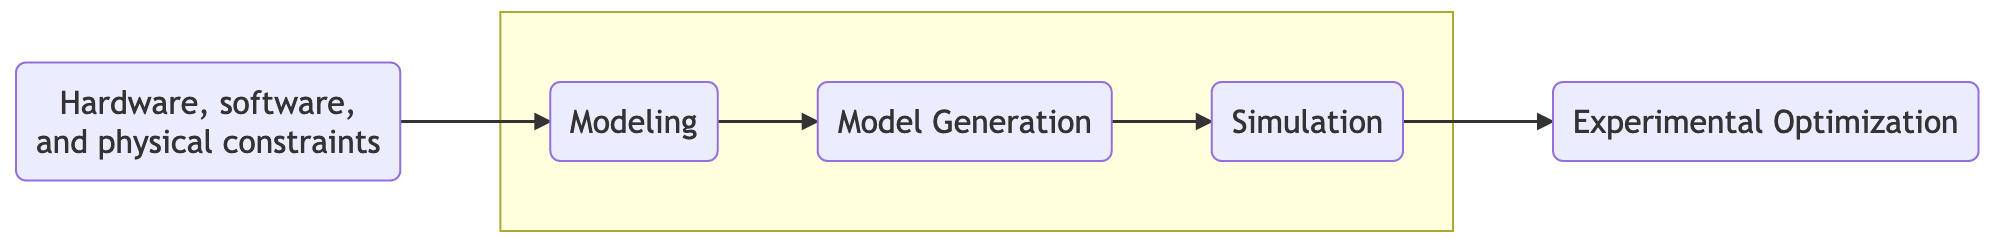
\includegraphics[width=0.95\textwidth]{images/mod_sim_flowchart.png}
    \caption{The high level flowchart capturing the modeling, simulation, and optimization process}
    \label{fig:mod-sim-flowchart}
% graph LR
%   model(Modeling)
%   modgen(Model Generation)
%   sim(Simulation)
%   opt(Experimental Optimization)
%   const(Hardware, software, <br> and physical constraints)

%   const --> model
%   subgraph " "
%     model --> modgen
%     modgen --> sim
%   end
%   sim --> opt
\end{figure}

%%%%%%%%%%%%%%%%%%%%%%%%%%%%%%%%%%%%%%%%%%
\subsection{Modeling}
The modeling was focused on hub-spoke and mesh networks. In each of the created models, each node represents the ESP8266 microcontroller-based physical devices, while the connections between the nodes represent the IEEE 802.11 based wireless communication. 

% Since the final design depends on the physical space, hardware, and software constraints of the project, the model was constructed with these constraints into consideration.%

According to our model, any two devices can only communicate if there is an established communication between them, and they are within each other's communication range. This models how wireless devices communicate with each other in the physical world. Given that the ESP8266 microcontrollers' built-in IEEE 802.11 based WiFi modules can typically connect with distances up to 100m \cite{chabukswardesign}, this is how we set the communication ranges for the nodes in our models.

Further, the number of simultaneous connections per device is also dependent on the hardware and software limitations. Since the ESP8266 microcontroller-based devices can have a maximum of eight simultaneous wireless connections \cite{ESP8266_NONOS_V1_1_0_Release_Notes}, the connection limit per node in our models follows this constraint as well. To achieve this, our model allows a maximum of four connections.

Although using regular nodes is enough to create a mesh network, there need to be "hubs" in order to create a hub-spoke network topology. The hubs were modeled as special nodes that can handle a larger number of simultaneous connections in the network. It was also assumed that the hubs are connected to each other with low-latency and high-speed communication mediums, as is often the case in a typical home network where routers are connected in this manner. 

In using the aforementioned "nodes" and "hubs", different network models were generated to represent various real-life network conditions. The next subsection explains how these models are generated.


%%%%%%%%%%%%%%%%%%%%%%%%%%%%%%%%%%%%%%%%%%
\newpage
\subsection{Model Generation}
\label{model-gen-section}
First, a two-dimensional rectangular virtual space was created based on the physical space constraints. The virtual space was configured to be flexible in terms of dimensions to accommodate different physical space requirements. Later, the target number of nodes were placed into the virtual space randomly using Python's \cc{randint()} method in order to prevent possible biases, as shown in \ref{fig:modeling_node}.

\begin{figure}[H]
    \centering
    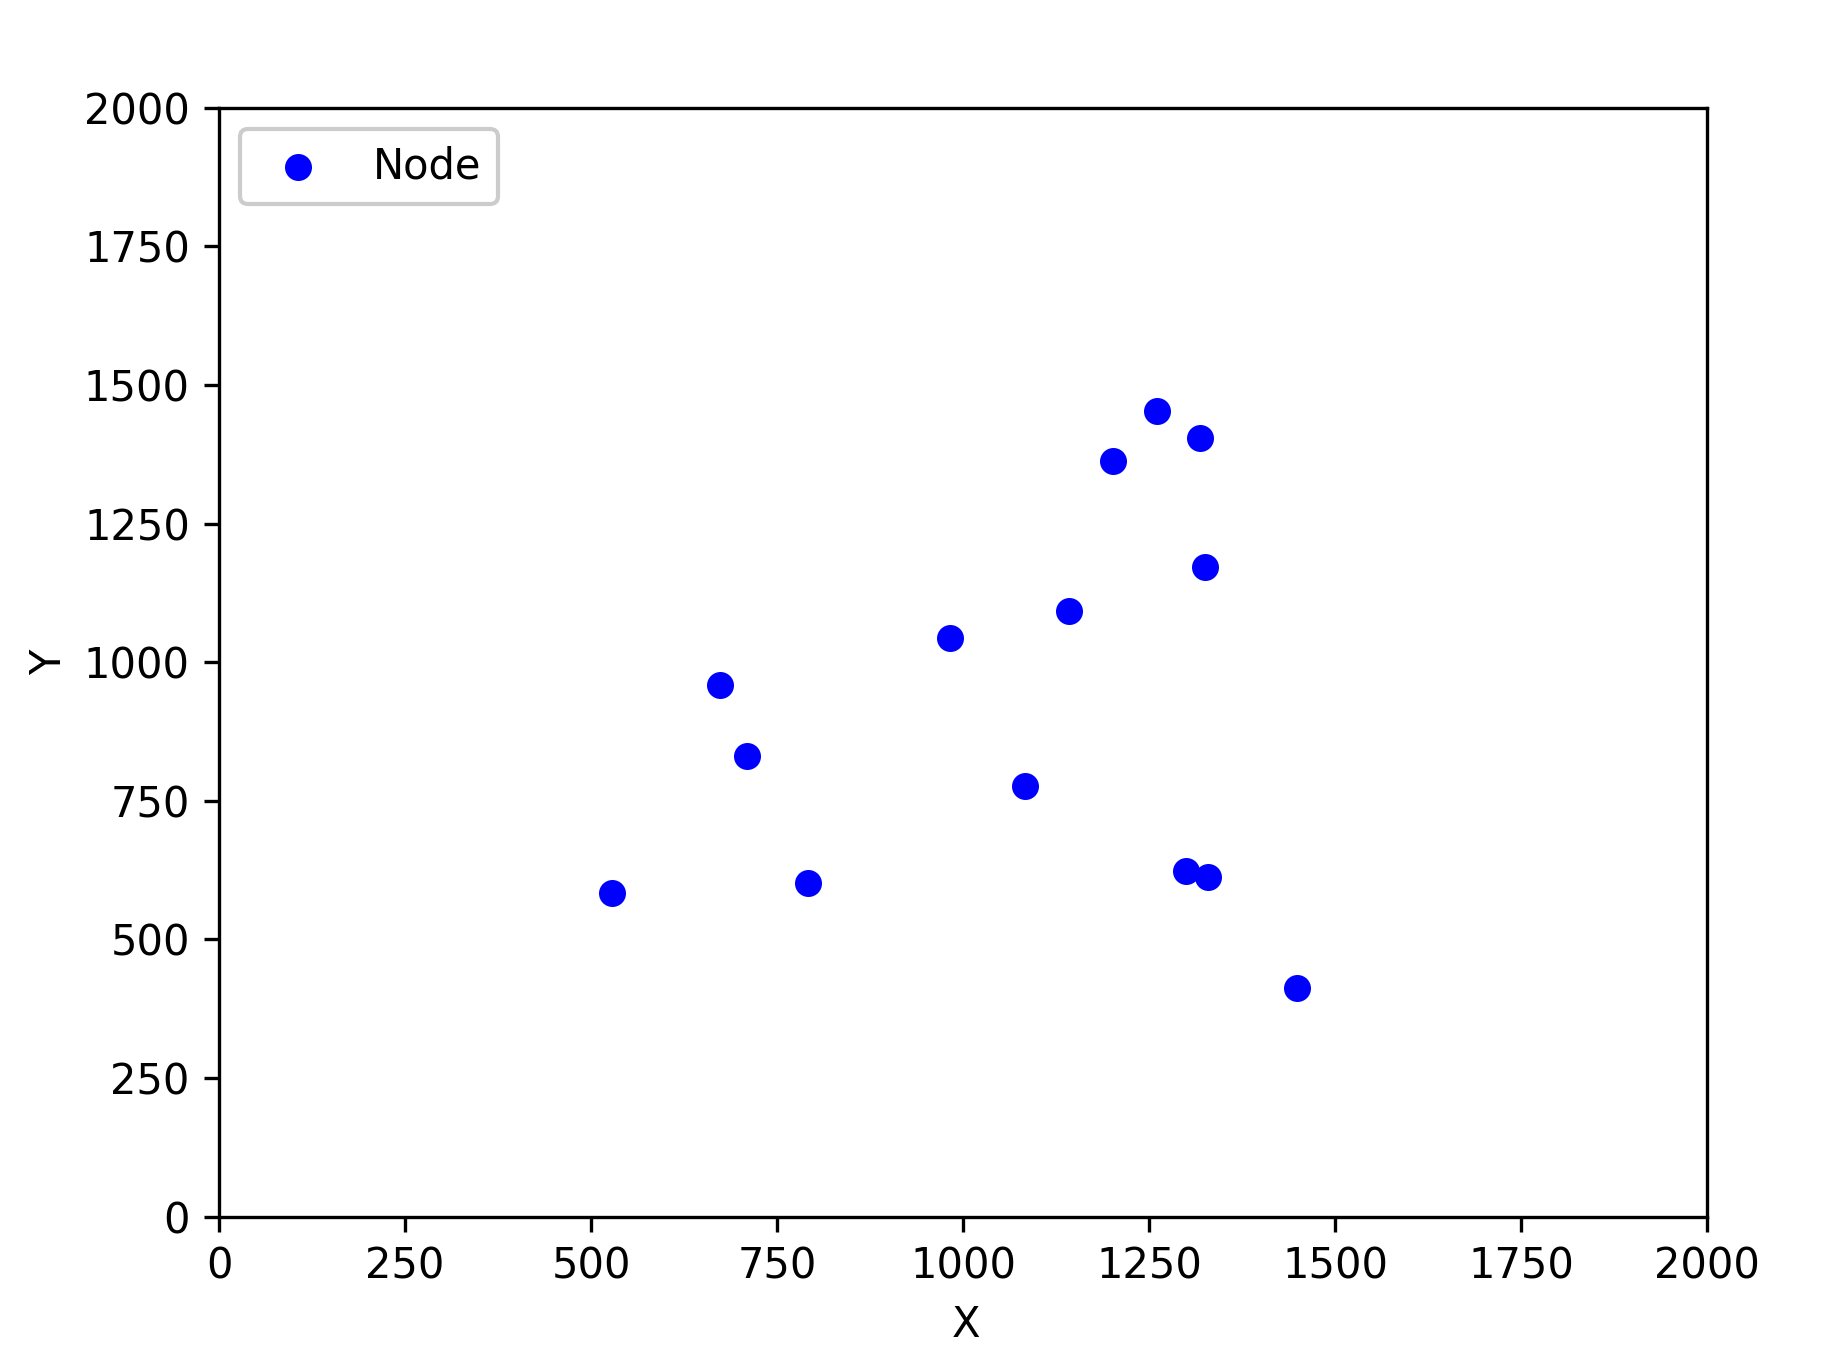
\includegraphics[width=0.42\columnwidth]{images/modeling_nodes_only.png}
    \caption{Nodes randomly distributed in the virtual space}
    \label{fig:modeling_node}
\end{figure}


Once the placement was completed in Figure \ref{fig:modeling_node}, the communication range of each node was determined within the virtual space, as shown in Figure \ref{fig:modeling_mesh}. Based on the simultaneous connection budget available for each node and overlapping communication ranges, the connections between the nodes can be created to construct a mesh network, as shown in Figure \ref{fig:modeling_mesh}.

\begin{figure}[H]
    \centering
    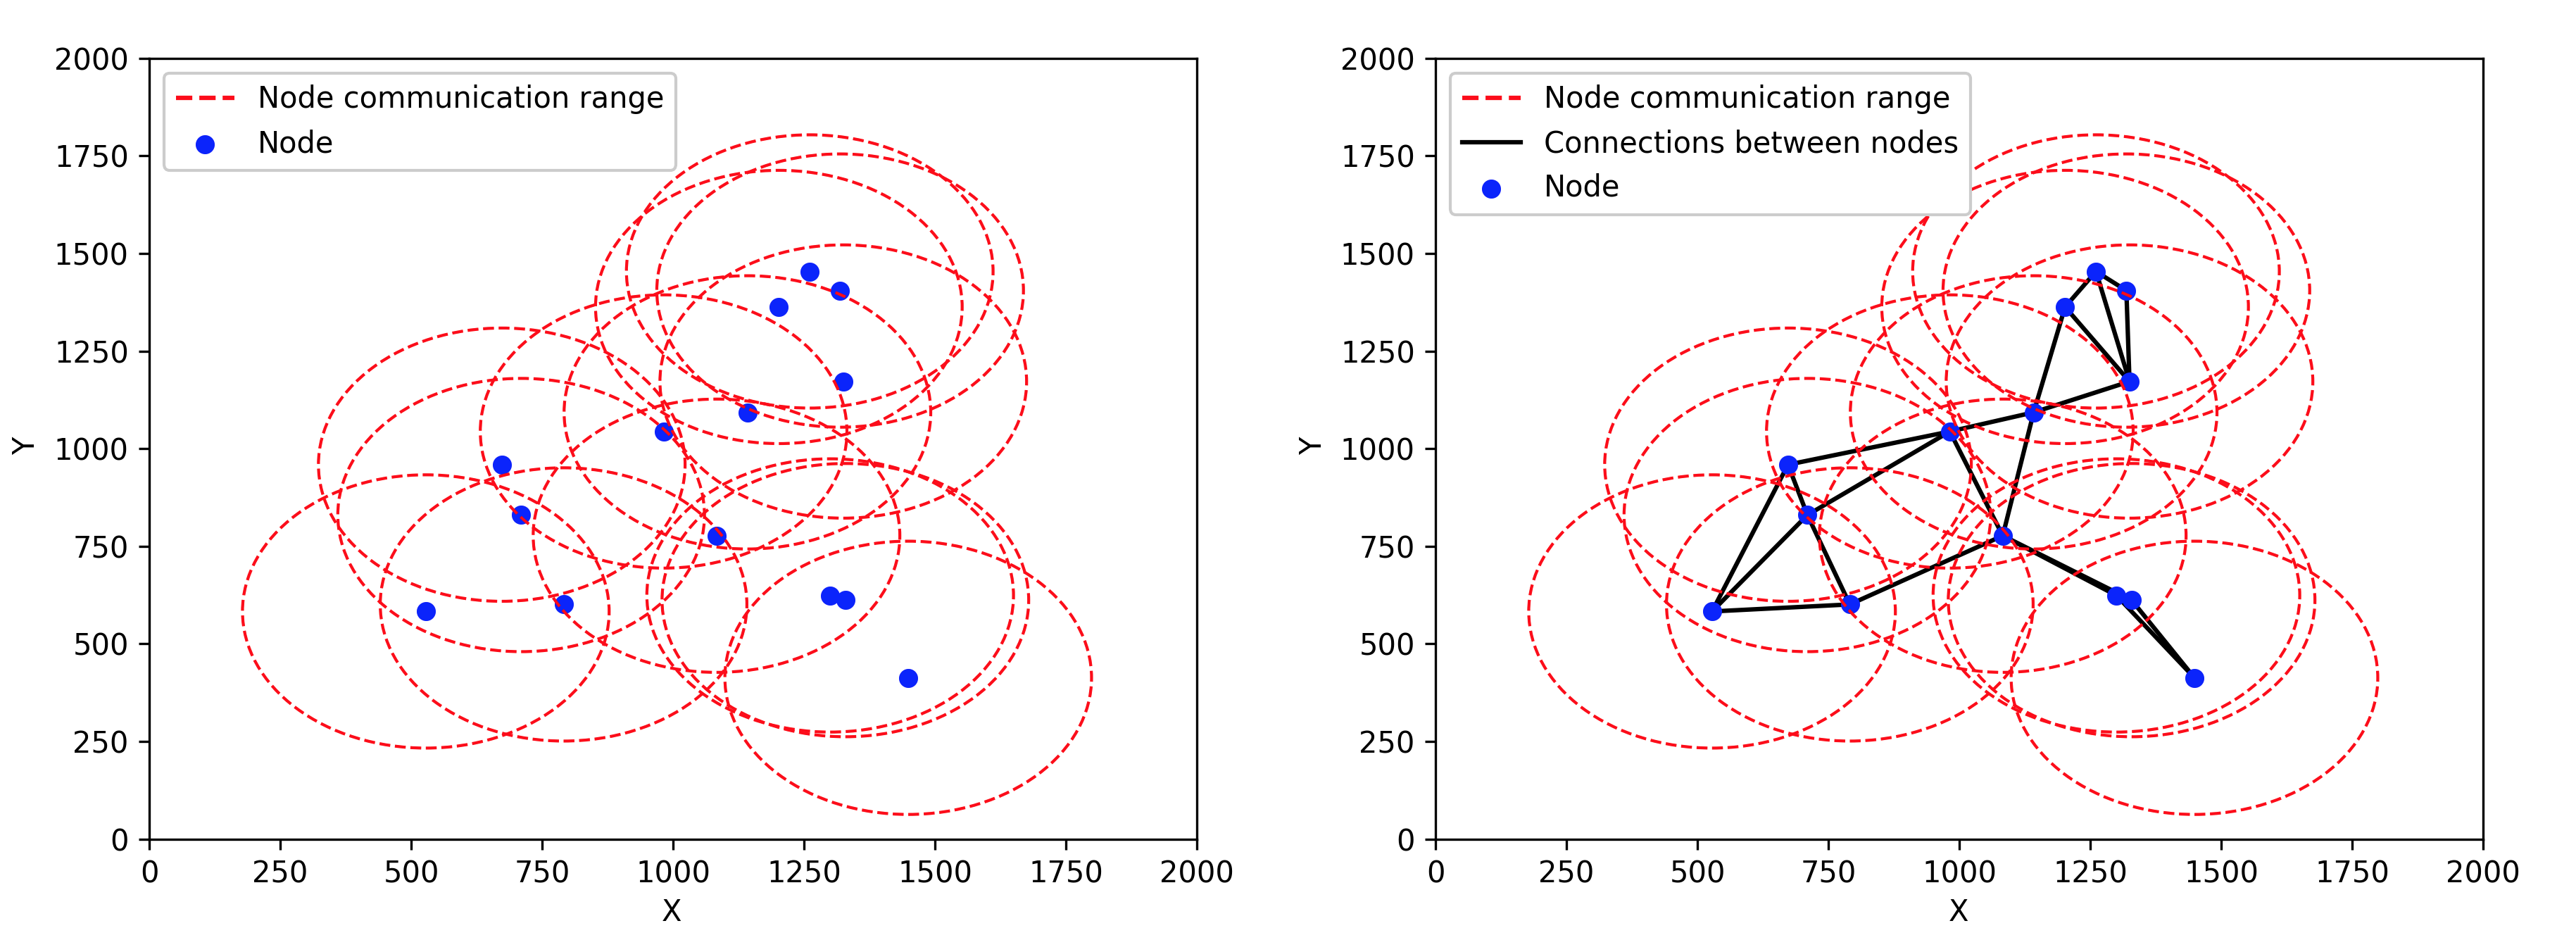
\includegraphics[width=0.88\columnwidth]{images/modeling_mesh.png}
    \caption{Left: Nodes and their communication ranges, Right: Nodes connected in mesh network topology based on the communication ranges}
    \label{fig:modeling_mesh}
\end{figure}

A hub-spoke network was also created from the random node placement shown in Figure \ref{fig:modeling_node}. However, it was not enough to simply check for the connection budget and overlapping communication ranges to construct a hub-spoke network topology, as was done for the mesh network. The nodes must communicate with each other via hubs. In order to find the optimal placement of the hubs for the created network, the "k-means" algorithm was applied iteratively until the created group of nodes covered the entire network. Next, a hub was placed at the center of each group, as shown on the left in Figure \ref{fig:modeling_star}. Nodes were then connected to the hubs, as shown on the right in Figure \ref{fig:modeling_star}.

\begin{figure}[H]
    \centering
    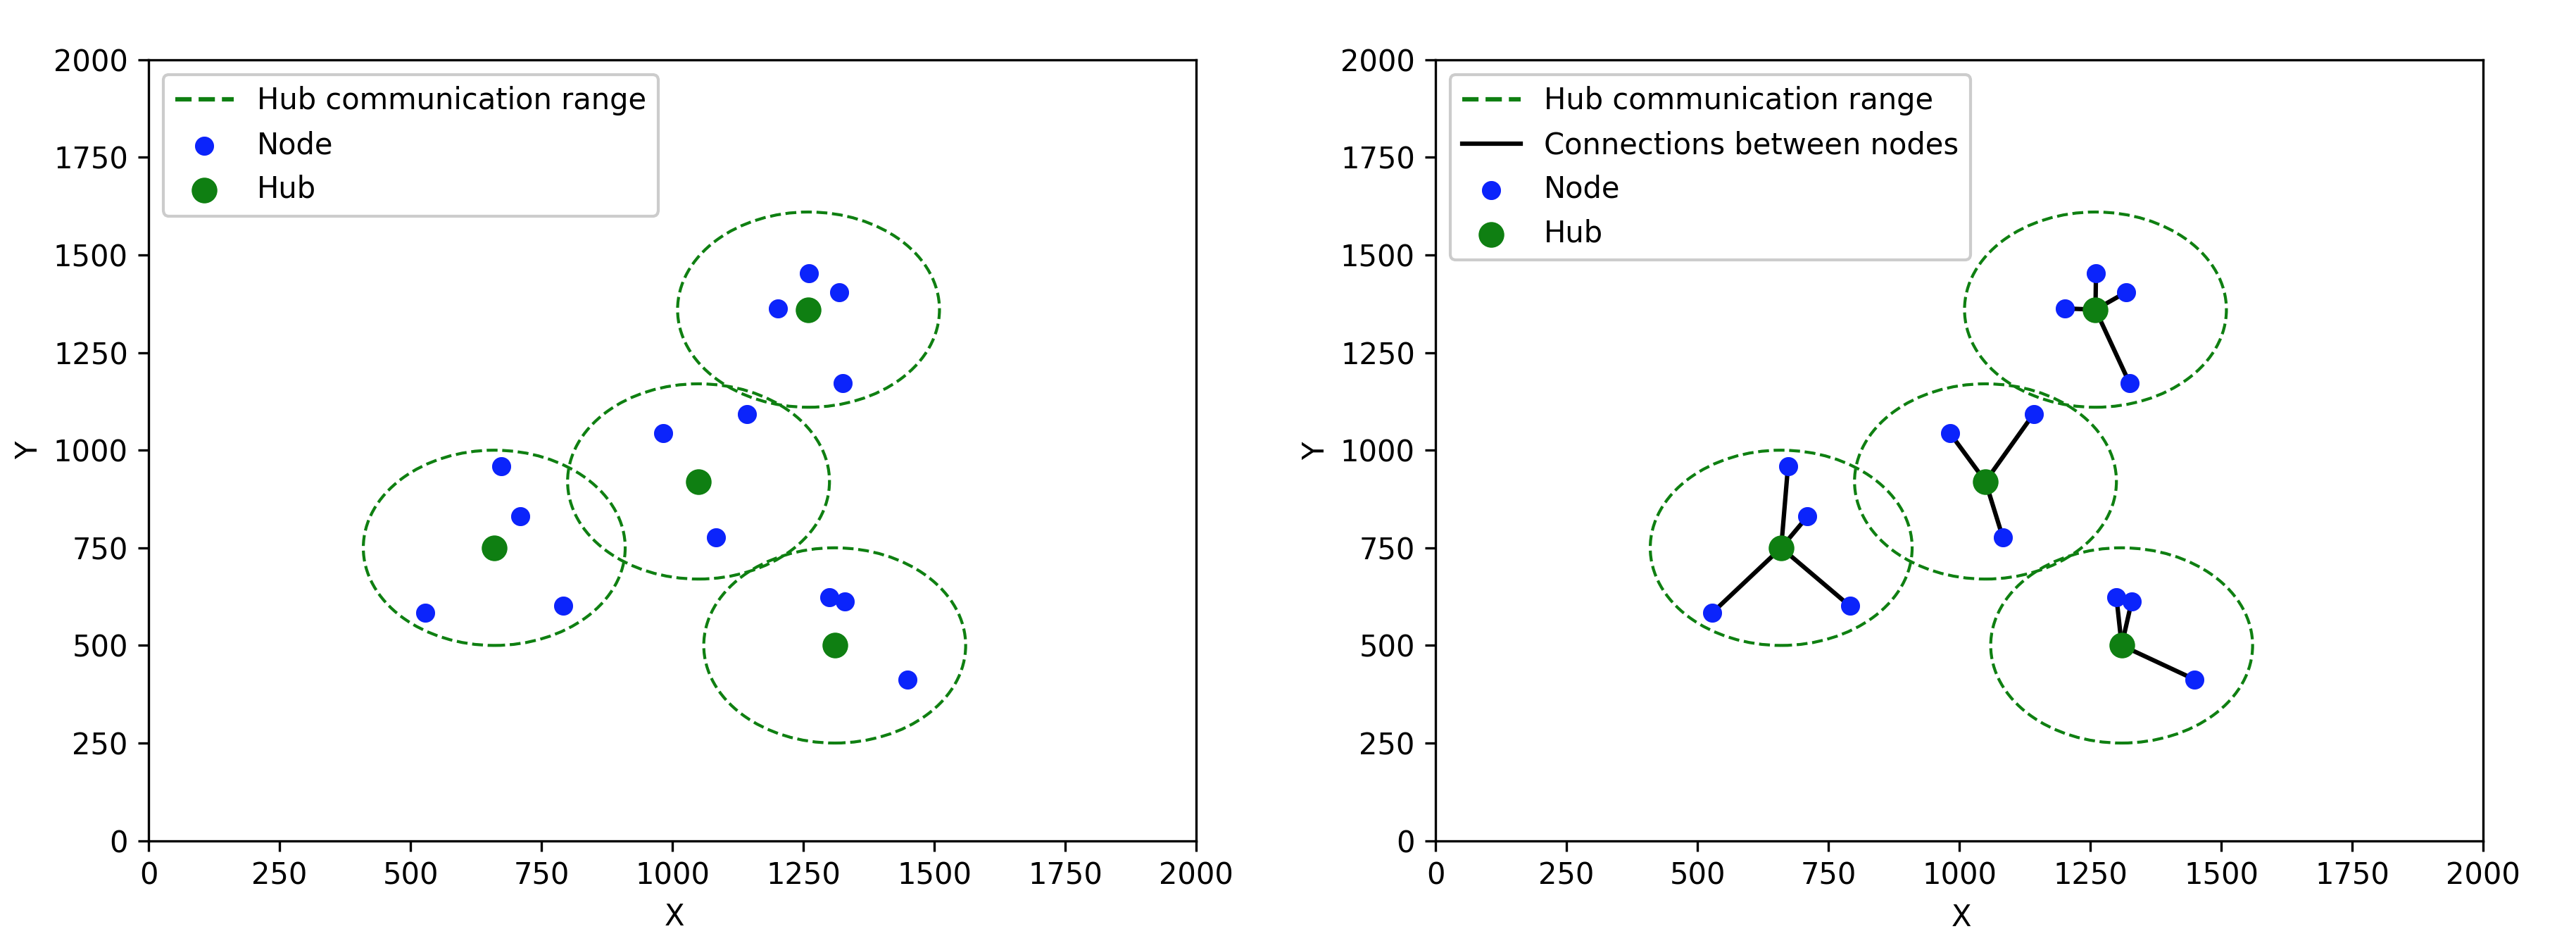
\includegraphics[width=0.88\columnwidth]{images/modeling_star.png}
    \caption{Left: Grouped nodes and corresponding hubs, Right: Nodes connected in hub-spoke (star) network topology based on the communication ranges}
    \label{fig:modeling_star}
\end{figure}

Figure \ref{fig:modeling_complex} demonstrates that the node placement process can be repeated with a greater number of nodes, different communication ranges \& budgets to create more complex hub-spoke and mesh networks
\begin{figure}[H]
    \centering
    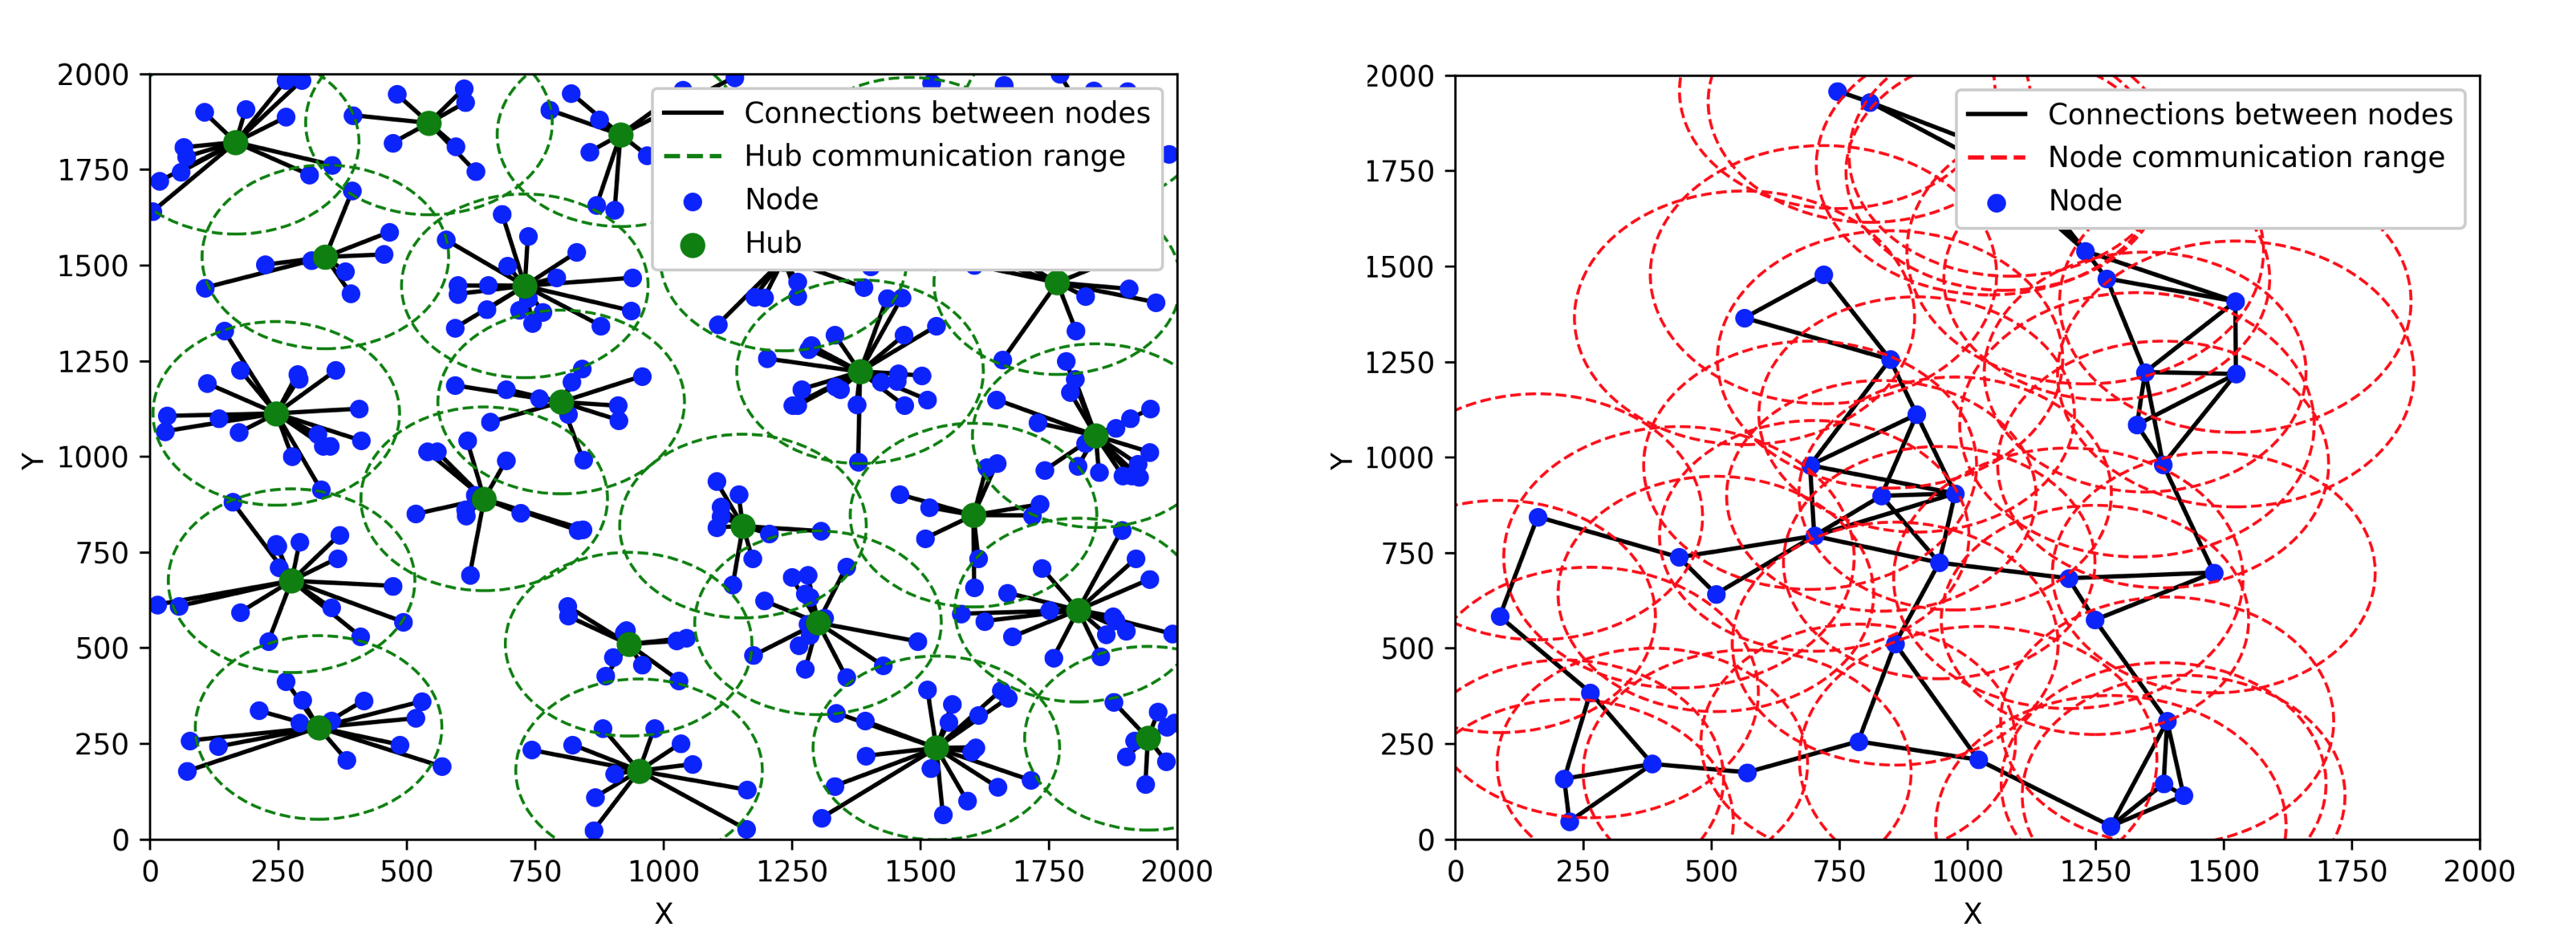
\includegraphics[width=0.88\columnwidth]{images/modeling_complex_unified.png}
    \caption{Left: Hub-spoke (star) network topology created in the virtual space, Right: Mesh network topology created in the virtual space}
    \label{fig:modeling_complex}
\end{figure}

The constructed models and the relations between the nodes and hubs in these models were exported for network communication simulations.

% talk about using python script to output x, y, z parameters (refer to it as \cc{network_generator} script)



%%%%%%%%%%%%%%%%%%%%%%%%%%%%%%%%%%%%%%%%%%
\subsection{Simulation and Experimental Results}

\subsubsection{Coracle Simulation}

We identified Coracle \cite{Coracle} as a tool to simulate the Raft consensus algorithm on heterogeneous networks. Coracle is a simulation framework written in the OCaml programming language, designed to evaluate "distributed consensus algorithms in settings that more accurately represent realistic deployments" \cite{howardCoracleEvaluatingConsensus2015}. The framework allows users to configure nodes, links, and events. 

A node can be defined as a hub, server, or client. From experimentation with the framework, we have learned that in the case of a server node, the node acts as a participant and carries out the responsibilities of a typical node, such as voting and log replication. When a node is configured as a hub, it foregoes its responsibility as a participant and acts as a router in the network. Finally, a client node is responsible for generating network traffic within the network between other clients \cite{howardCoracleEvaluatingConsensus2015}. Using the models generated, as described in section \ref{model-gen-section}, we set the routers in the hub-spoke topology to be hubs and set the remaining nodes to be servers. In the special case of a mesh topology, the nodes had to perform the role of a server and a hub simultaneously. Since Coracle does not allow for a node to hold two roles, we split each modeled node into two nodes: a hub node that maintained the modeled mesh connections and a server node that handled consensus actions. This way, we were able to emulate each node as having a very limited routing capability (maximum four connections), as is the case with ESP8266 chips.

In Coracle, links can either be unidirectional or bidirectional; moreover, multiple links between two nodes can exist. Essentially, this allows for the freedom to simulate whether a pair of nodes have half-duplex or full-duplex communication. Furthermore, each link can be assigned a latency category, small, medium, or large, to affect the package delivery time from source to destination nodes. \cite{howardCoracleEvaluatingConsensus2015}. For the sake of simplicity in our simulations, we modeled each link to have a small latency.

Events allow for nodes and links to activate or deactivate at user-defined timestamps. This can simulate unstable networks with multiple unreliable links that periodically fail. Moreover, considering real-world networks, this parameter can also be used to simulate the addition of new nodes into the network, with the only limitation being that node links would be predetermined \cite{howardCoracleEvaluatingConsensus2015}. To test the recovery ability between mesh and hub-spoke networks, we added a \cc{down hub time} parameter that brought down a random router in the network at the specified time. 

A limitation in the modeling and simulation workflow is the lack of traveling nodes, which rebuild their links based on available nearby nodes. However, we were able to test this with our library.

Coracle accepts a JavaScript Object Notation (JSON) file with a specific structure as an input. We wrote a \cc{simulation\_configuration} script to process the generated network models described in Section \ref{model-gen-section} and generate a JSON file based on the network parameters. Next, we wrote a \cc{run\_coracle} script to feed the generated JSON file into Coracle and gather the results. Finally, we wrote a \cc{experiment\_suite} script that generated multiple networks based on the desired number of nodes and area size, ran each network 100 times, and visualized these results.

\subsubsection{Results}
\label{sec:coracle_results}

Using Coracle, we were able to simulate several scenarios in order to justify the use of a mesh network in a consensus algorithm, as well as inform the configuration of our implementation. 

Figure \ref{fig:simulation_result_100} shows the results of a network simulation in a 10000 $unit^2$ area for both star and mesh topologies. The remaining graphs, which vary the number of nodes per area, can be found in Appendix \ref{sec:appendix-for-coracle-results}. In this scenario, the simulations ran for 1000 milliseconds each, and a random router was brought down for 200 milliseconds at the halfway mark (500 milliseconds). For each graph, we ran 100 simulations and gathered the generated statistics to inform our design.

\begin{figure}[H]
    \centering
    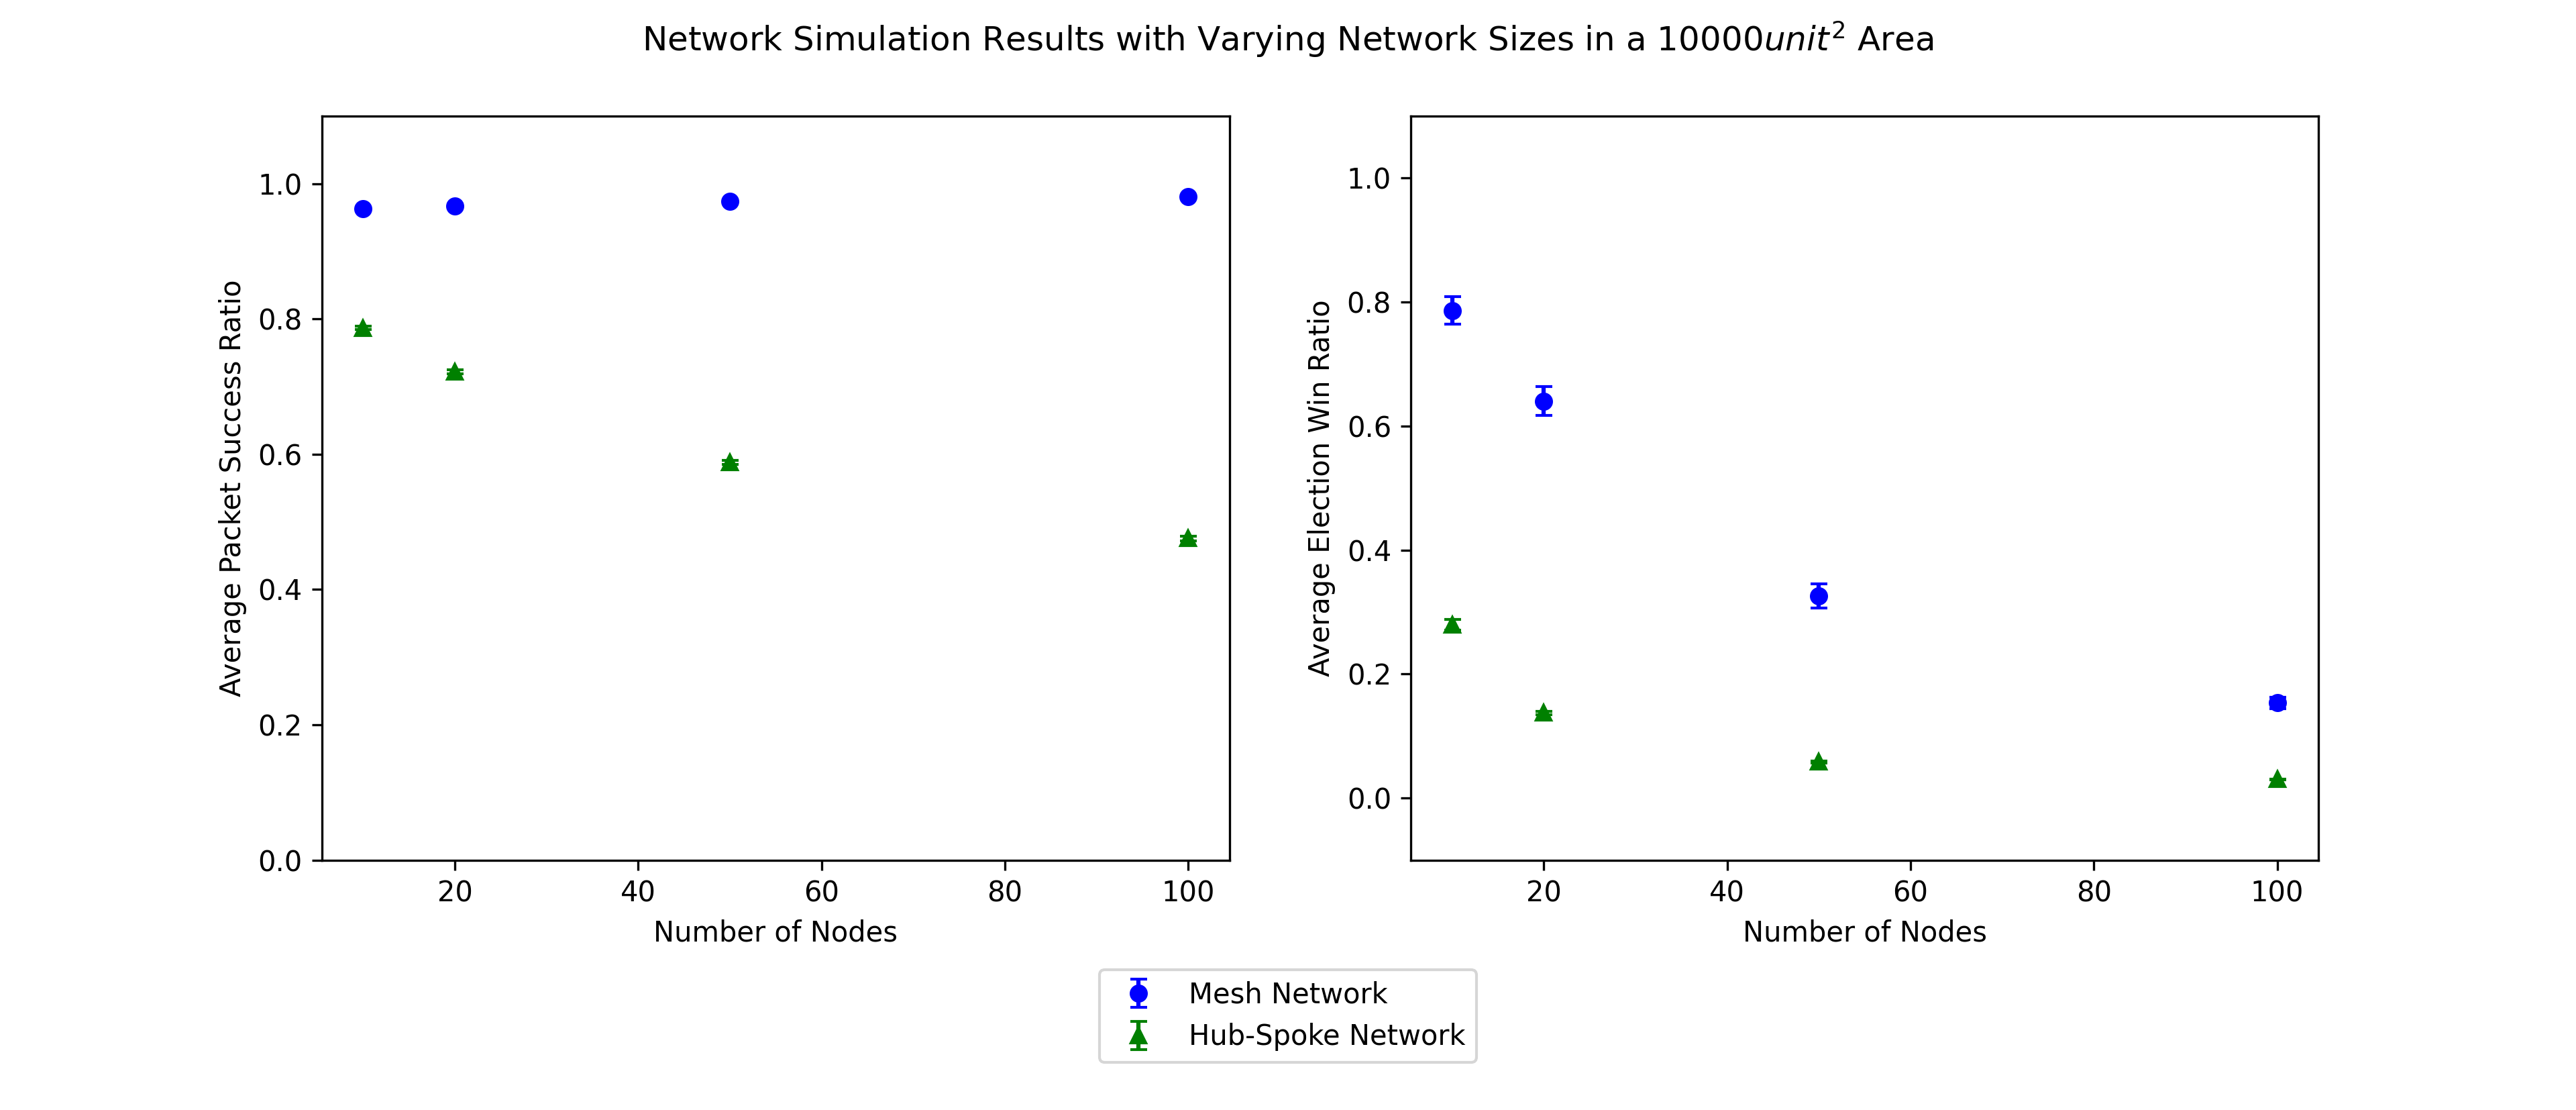
\includegraphics[width=0.9\columnwidth]{images/100unit^2.png}
    \caption{Left: Average packet delivery success ratio per number of nodes, Right: Average ratio of elections won to initiated per number of nodes }
    \label{fig:simulation_result_100}
\end{figure}

Given the results from Figure \ref{fig:simulation_result_100} and those found in Appendix \ref{sec:appendix-for-coracle-results}, we suggest that a mesh network can better recover from abrupt changes to the system, which is characteristic of the dynamic network topologies of mobile systems.

We then used Coracle to further explore mesh networks by varying three main parameters: the number of nodes in the network, the duration between heartbeat messages sent by the consensus leader, and the upper bound of the election timeout. 

Figure \ref{fig:coracle_vary_nodes} shows the average time to first leader (ATFL) and the average ratio of elections won to initiated (AER) for various network sizes ($number\_of\_nodes$ $ = $ $[3,$ $5,$ $10,$ $20,$ $30,$ $50,$ $80,$ $100]$). Here the heartbeat interval was constrained to 30 milliseconds and the election timeout range was set between 60-300 milliseconds.

\begin{figure}[H]
    \centering
    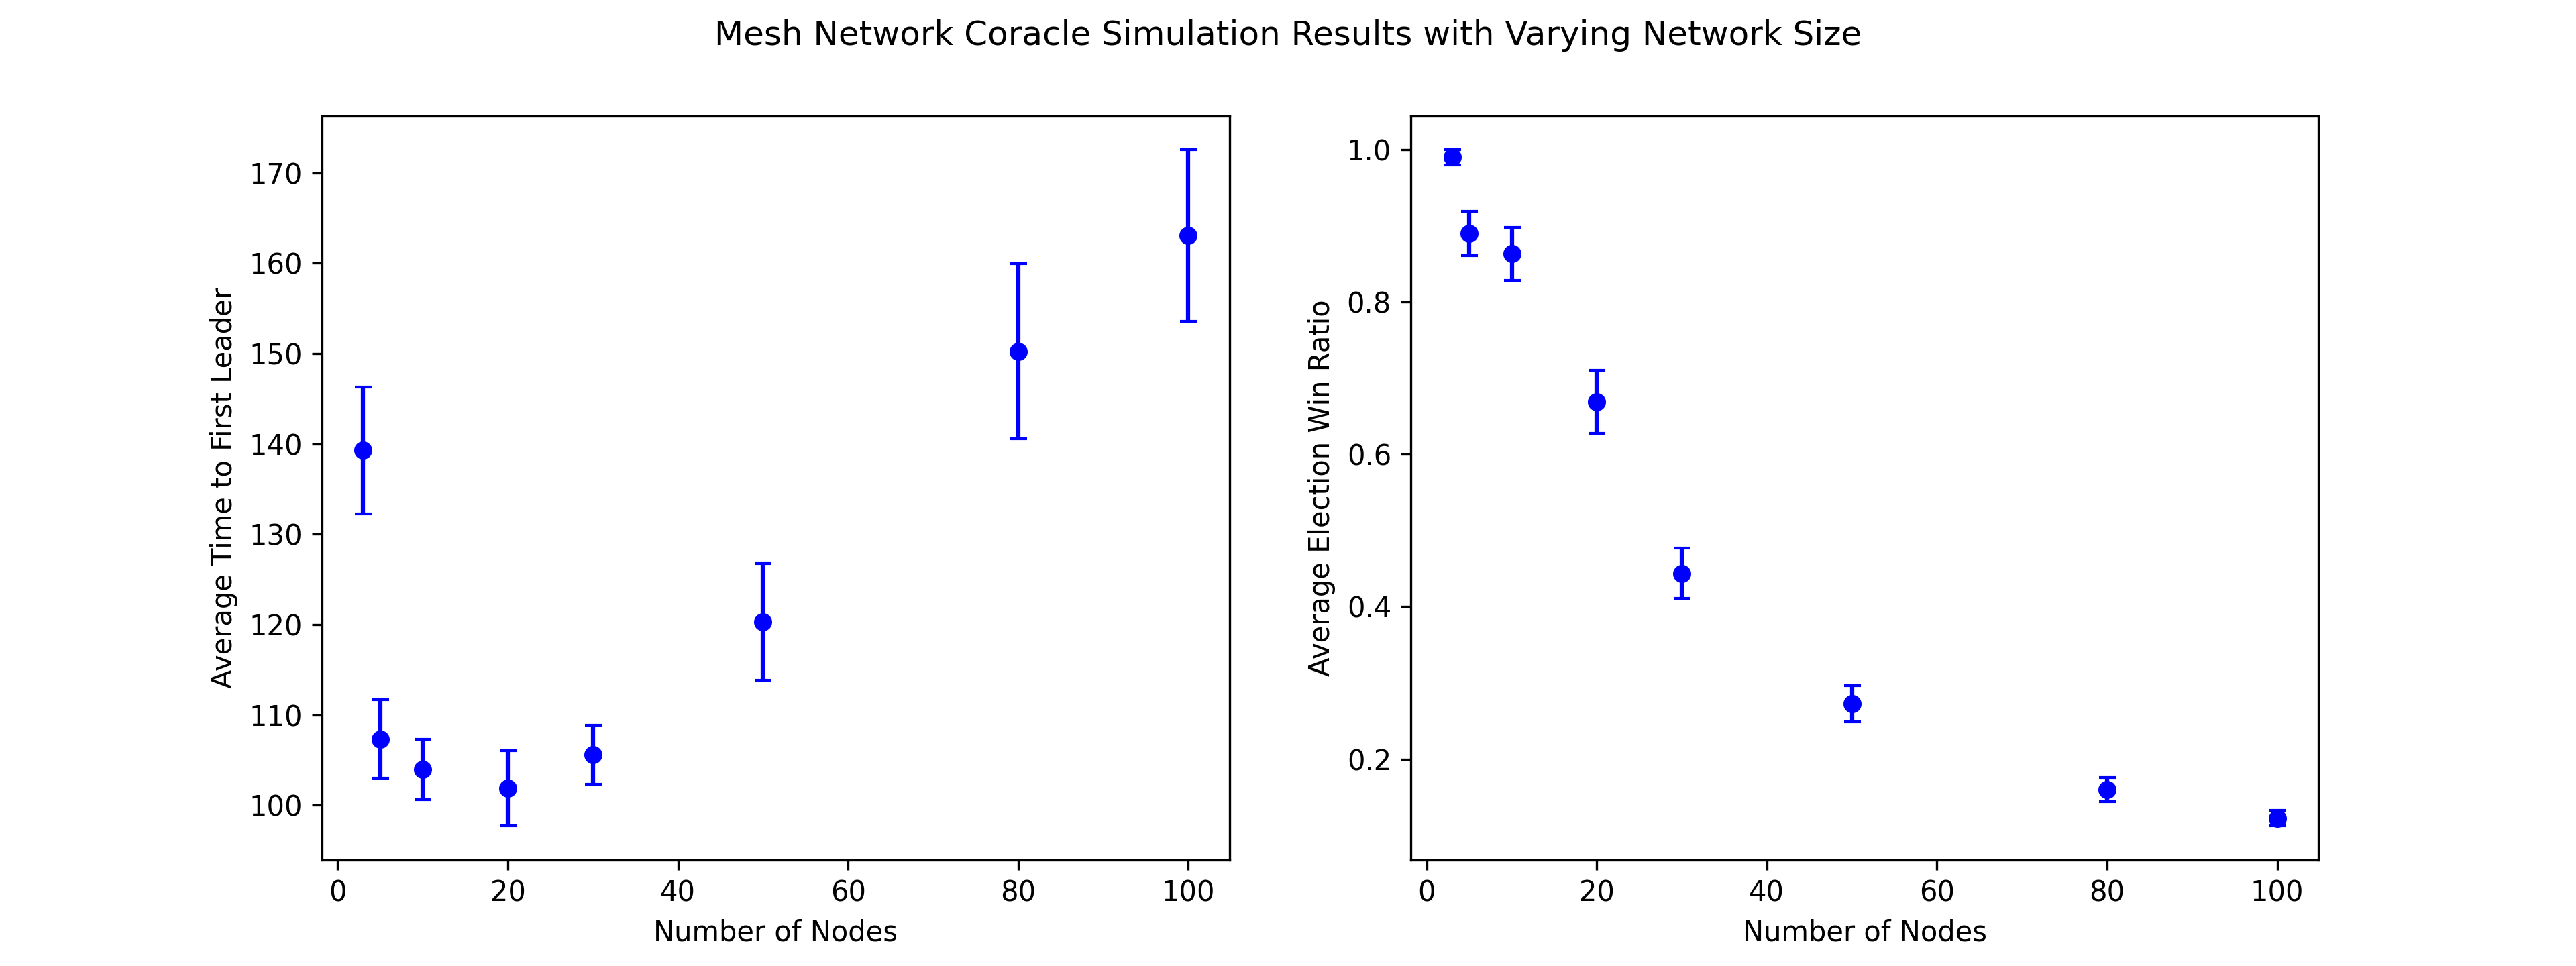
\includegraphics[width=0.9\columnwidth]{images/coracle_vary_nodes.png}
    \caption{Left: Average time to first leader per number of nodes, Right: Average ratio of elections won to initiated per number of nodes}
    \label{fig:coracle_vary_nodes}
\end{figure}

The results clearly indicate that as the number of nodes increase, more elections tend to be wasted. Interestingly, the results also indicate that a network can be too small or too large in coming to an agreement over the selection of a leader. A small network may take too long to gain a majority vote, while a network too large may have difficulty in sending its vote requests out to the other nodes before they time out and start their own elections. 

Figure \ref{fig:coracle_vary_heartbeat} shows the results of varying heartbeat intervals ($heart\_beat\_periods$ $ = $ $[60,$ $120,$ $180,$ $240,$ $300,$ $360,$ $420,$ $480,$ $540,$ $600,$ $660,$ $720]
$) to test for ATFL and AER. In these simulations, the network size was set to 20 nodes and the election timeout range was set between 60-300 milliseconds.

\begin{figure}[H]
    \centering
    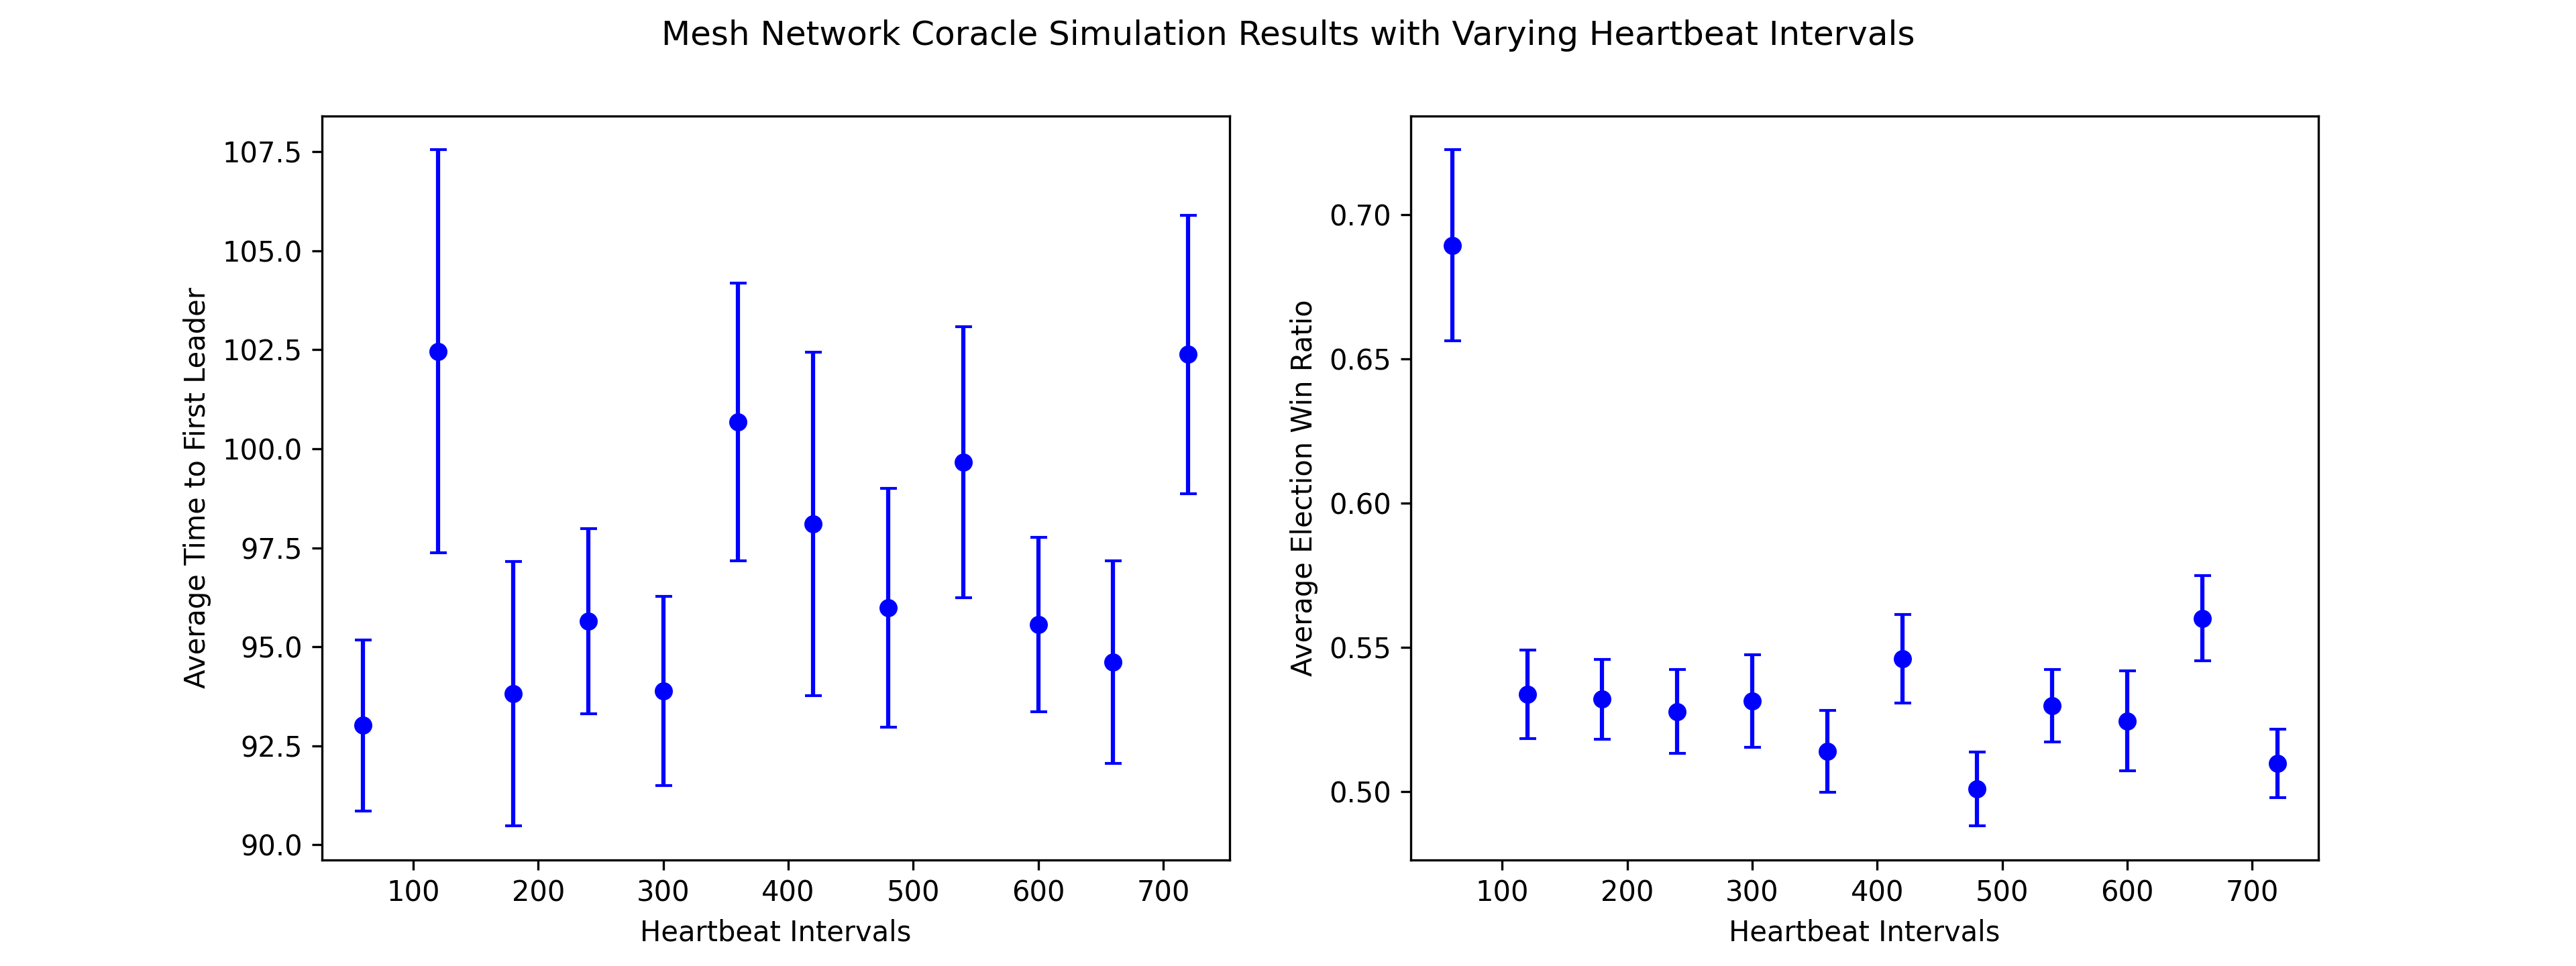
\includegraphics[width=0.9\columnwidth]{images/coracle_vary_heartbeat.png}
    \caption{Left: Average time to first leader per change in heartbeat interval, Right: Average ratio of elections won to initiated per change in heartbeat interval }
    \label{fig:coracle_vary_heartbeat}
\end{figure}

There is no clear answer as to whether varying heartbeat intervals has a significant effect on the ATL; however, 60 milliseconds is clearly the optimal time when looking at AER. Since the difference in AER between a network using 60 milliseconds and 120 milliseconds is so large, we hypothesize that this may actually be a result of how Coracle was implemented and how time is handled in the simulation.

Finally, Figure \ref{fig:coracle_vary_election_timeout} shows the results of varying the upper-bound of the election timeout, effectively increasing the average time it takes for a node to timeout and switch from a follower to a candidate state. Here, the heartbeat interval was fixed to 30 milliseconds while the network size was limited to 20 nodes.

\begin{figure}[H]
    \centering
    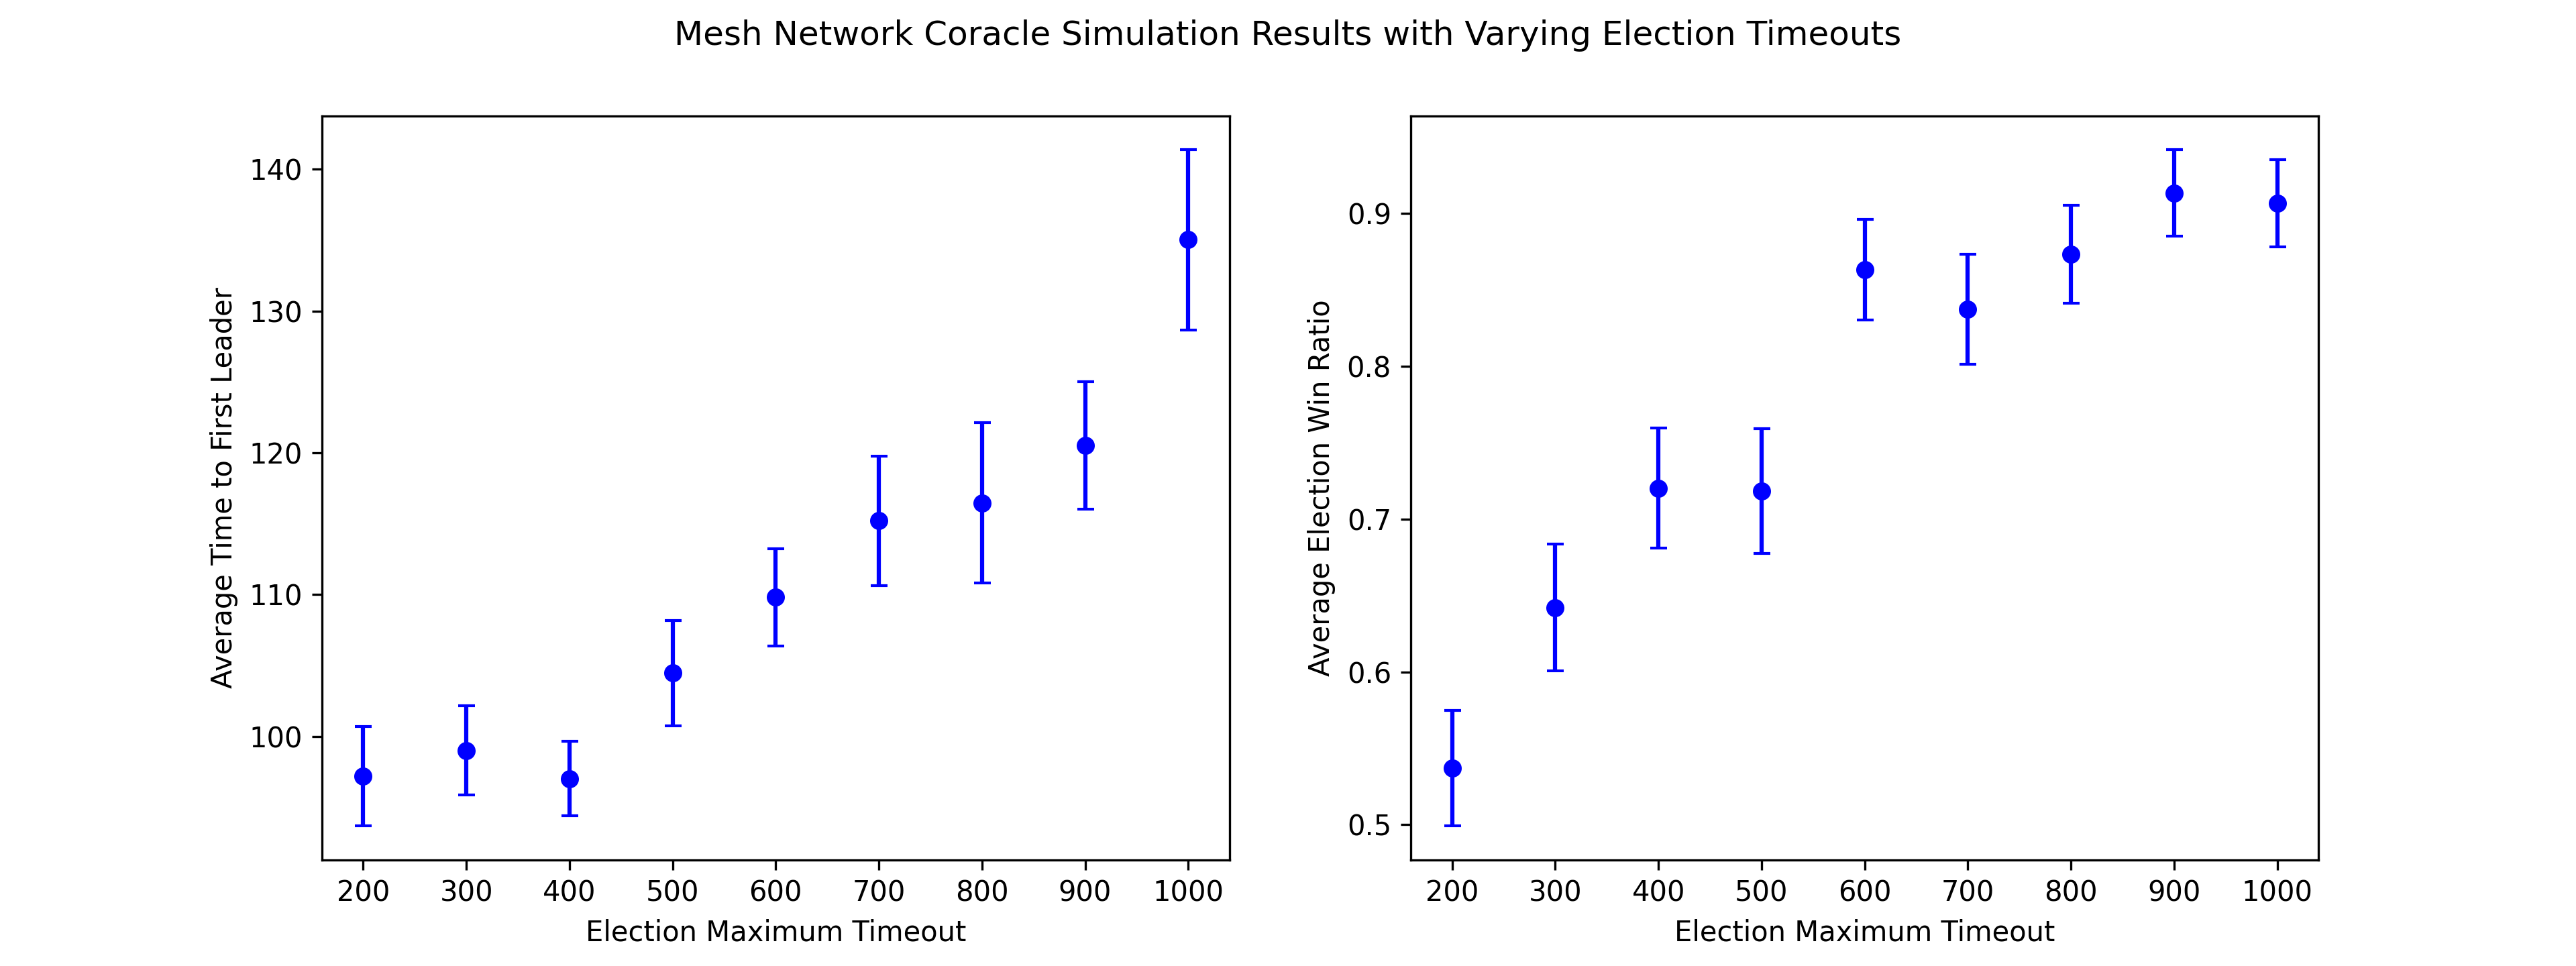
\includegraphics[width=0.9\columnwidth]{images/coracle_vary_election_timeout.png}
    \caption{Left:Average time to first leader per change in maximum possible election timeout, Right: Average ratio of elections won to initiated per change in maximum possible election timeout}
    \label{fig:coracle_vary_election_timeout}
\end{figure}

The results in Figure \ref{fig:coracle_vary_election_timeout} seem to indicate that a large election maximum timeout, which translates to a greater average election timeout, is always better: both the ATL and AER increase as the timeout period increases. However, a large election timeout pushes the network to behave in a more centralized way. A large election timeout would be detrimental to a system where the leader may quickly fall out of the network because the other nodes would be slow to step in for a chance at becoming the leader. Large gaps between leaders will fill the data buffers of the nodes, creating a backlog that could overload the network.

Overall, visualizing how the network reacts to changes in certain parameters helped inform us on how to select the parameters for our implementation. Section \ref{sec:optimization_performed} details how we used these results in our system.

%%%%%%%%%%%%%%%%%%%%%%%%%%%%%%%%%%%%%%%%%%
\subsection{Optimization Performed}
\label{sec:optimization_performed}

We followed the experimental plan below to optimize our software library:
\begin{enumerate}
    \item Using NetworkX and SciKits software libraries, we generated models for star and mesh network topologies in virtual spaces.
    \item We ran Coracle simulations on the network models, adjusting for different parameters such as range, the maximum distance between nodes, maximum concurrent connections, virtual space, election timeouts, heartbeat intervals, and link failure rate.
    \item Informed with the theoretical limitations of Raft and practical limitations of painlessMesh, we wrote our consensus on mesh software library.  
    \item Throughout implementing our software library, we tested modules of the library on ESP8266 development boards and on a virtual network of nodes to obtain satisfactory results.
    \item We designed a virtual testing framework that tested a range of parameters similar to those that worked well in Coracle simulations
    \item We used the results of our virtual testing framework to inform the final configuration of our software library.
\end{enumerate}

The modeling and simulations we performed guided us while making the design choices while implementing our software library. In the Coracle simulations, we defined the resilience of a network by three parameters: average packet delivery rate, the average time to the first leader, and average election win to initiated ratio. In using the simulations, our efforts were focused on understanding the Raft parameters, such as typical election timeout and heartbeat frequency, on maximizing packet delivery and minimizing unnecessary elections. As a result, we gained an understanding of the range of environments in which our physical system will have effective use.

%%%%%%% FINAL DESIGN %%%%%%%
\newpage
\section{Final Design}

\subsection{Initial Design Proposed}

As delineated in Table \ref{tab:final_design_chart_options}, the final design will use the Raft consensus algorithm on an IEEE 802.11 based mesh topology using the painlessMesh networking library on an ESP8266 microcontroller.

\begin{table}[H]
    \centering
    \footnotesize
    \renewcommand{\arraystretch}{1.2}
    \vspace{10pt}
    \caption{The sub-problems of the final design and chosen options}
    \label{tab:final_design_chart_options}
    \begin{tabular}{|c|c|}
        \hline
        \textbf{Sub-Problem}   & \textbf{Chosen Option}  \\ 
        \thickhline 
        Networking Protocol    &  IEEE 802.11            \\ \hline
        Networking Topology    &  Mesh Topology          \\ \hline
        Consensus Algorithm    &  Raft                   \\ \hline
        Microcontroller        &  ESP8266                \\ \hline
        Networking Library     &  painlessMesh           \\ \hline
    \end{tabular}
\end{table}

\vspace{-15pt}

Figure \ref{fig:final_design_node_bb} shows how nodes in the network will be communicating with each other in the final design.

\begin{figure}[H]
    \centering
    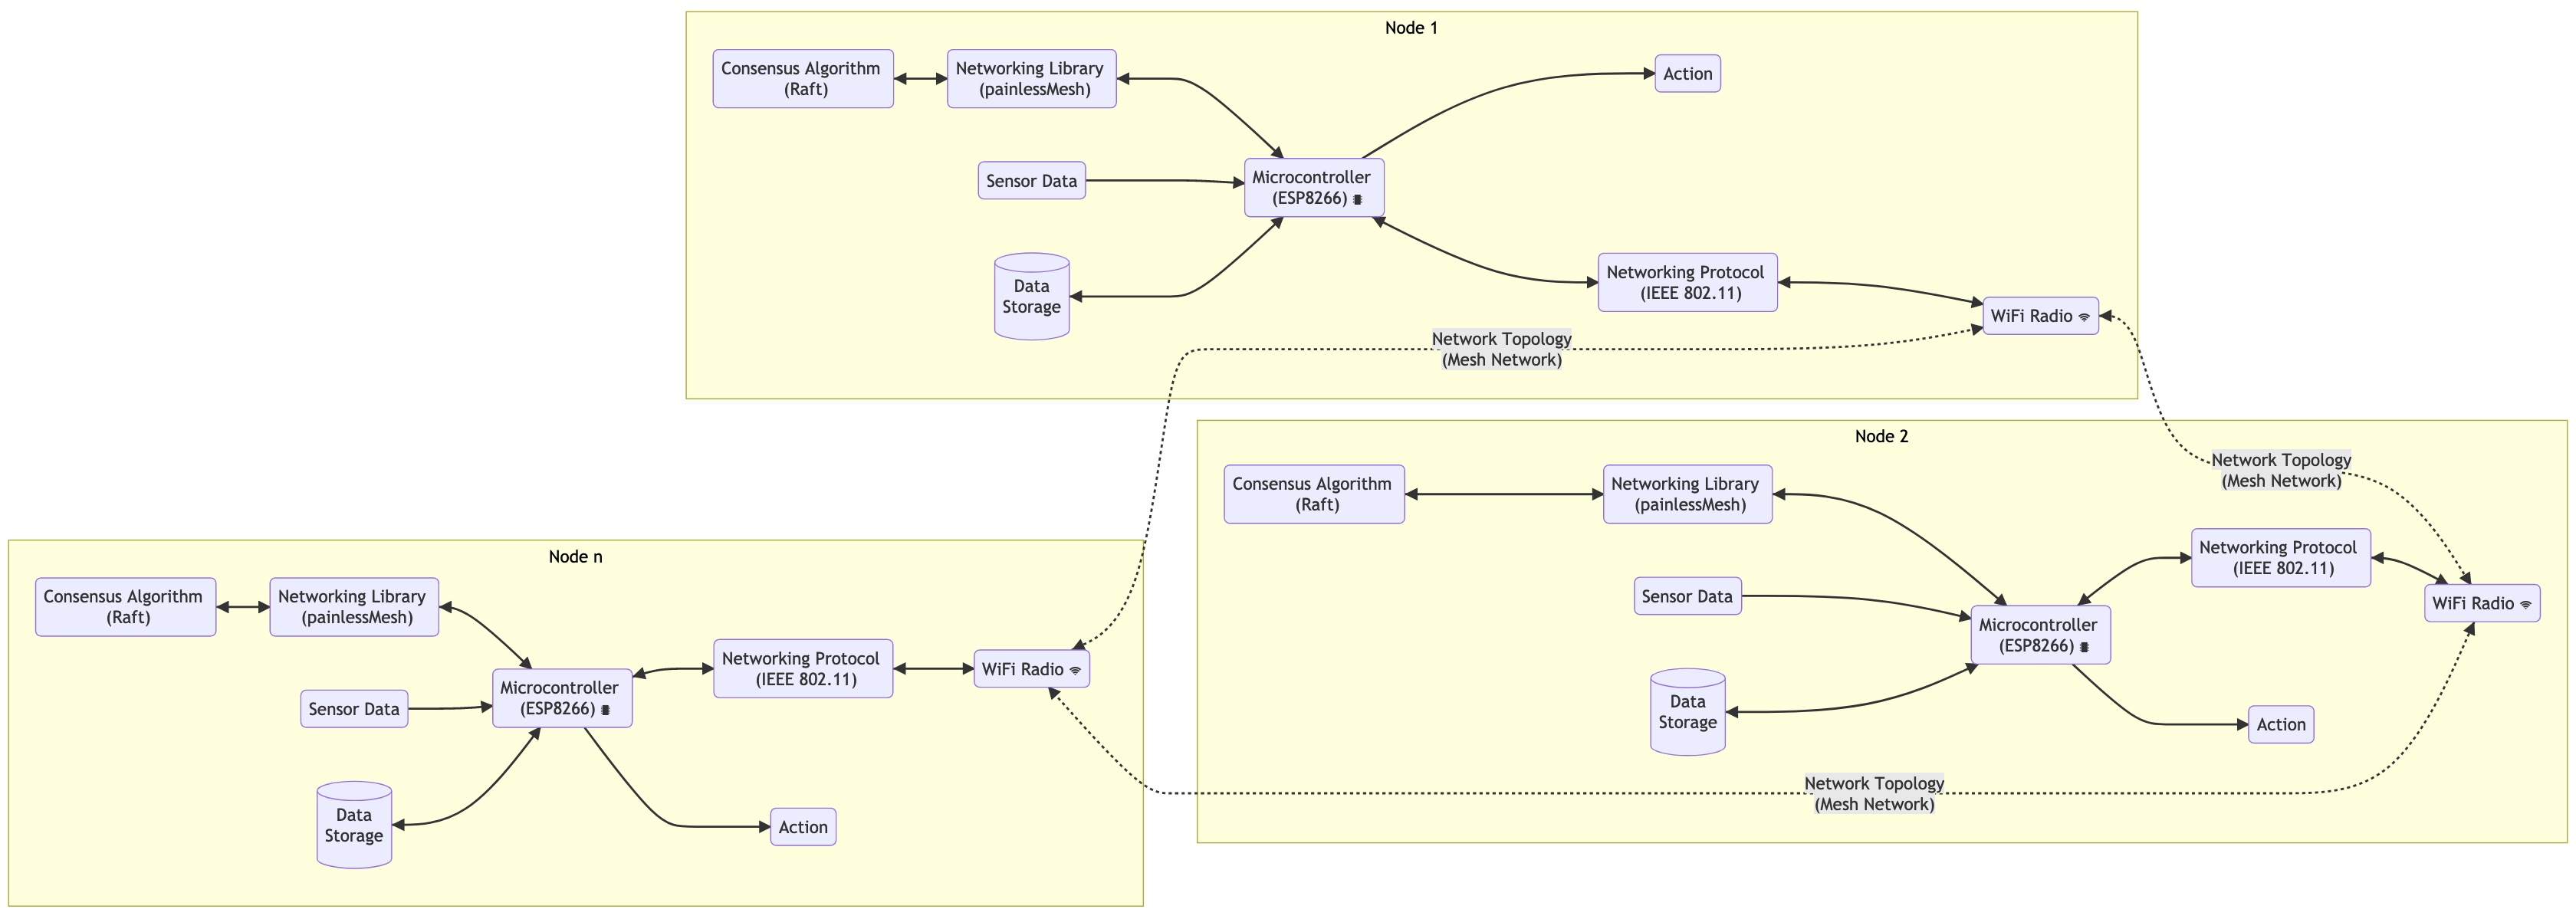
\includegraphics[width=1\textwidth]{images/final_design_nodes.png}
    \caption{Detailed black box of each node in the final design}
    \label{fig:final_design_node_bb}
    
% flowchart LR
%     1_radio  <-..-> |"Network Topology <br> (Mesh Network)"| 2_radio
%     2_radio <-.....->  |"Network Topology <br> (Mesh Network)"| n_radio
%     n_radio <-..->  |"Network Topology <br> (Mesh Network)"| 1_radio

%     subgraph 1[Node 1]
%       1_radio(WiFi Radio fa:fa-wifi)
%       1_cons("Consensus Algorithm <br> (Raft)")
%       1_netProc("Networking Protocol <br> (IEEE 802.11)")
%       1_netLib("Networking Library <br> (painlessMesh)")
%       1_cont("Microcontroller <br> (ESP8266) fa:fa-microchip")
%       1_act(Action)
%       1_sens(Sensor Data)
%       1_sto[(Data <br> Storage)]
%       1_sto <--> 1_cont
%       1_sens --> 1_cont
%       1_cont --> 1_act
%       1_cons <--> 1_netLib <--> 1_cont <--> 1_netProc <--> 1_radio
%     end

%     subgraph 2[Node 2]
%       2_radio(WiFi Radio fa:fa-wifi)
%       2_cons("Consensus Algorithm <br> (Raft)")
%       2_netProc("Networking Protocol <br> (IEEE 802.11)")
%       2_netLib("Networking Library <br> (painlessMesh)")
%       2_cont("Microcontroller <br> (ESP8266) fa:fa-microchip")
%       2_act(Action)
%       2_sens(Sensor Data)
%       2_sto[(Data <br> Storage)]
     
%       2_cons <--> 2_netLib <--> 2_cont <--> 2_netProc <--> 2_radio
%       2_sto <--> 2_cont
%       2_sens --> 2_cont
%       2_cont --> 2_act
%     end

%     subgraph n[Node n]
%       n_radio(WiFi Radio fa:fa-wifi)
%       n_cons("Consensus Algorithm <br> (Raft)")
%       n_netProc("Networking Protocol <br> (IEEE 802.11)")
%       n_netLib("Networking Library <br> (painlessMesh)")
%       n_cont("Microcontroller <br> (ESP8266) fa:fa-microchip")
%       n_act(Action)
%       n_sens(Sensor Data)
%       n_sto[(Data <br> Storage)]
%       n_sto <--> n_cont
%       n_sens --> n_cont
%       n_cons <--> n_netLib <--> n_cont <--> n_netProc <--> n_radio
%       n_cont --> n_act
      
%     end
\end{figure}


%%%%%%%%%%%%%%%%%%%%%%%%%%%%%%%%%%%%%%%%%%%%%%%%%%%%%%%
\vspace{-25pt}
\subsubsection{Microcontroller}
The final design will use ESP8266 microcontrollers to run the required consensus algorithm and perform the networking functionality with its built-in IEEE 802.11 based WiFi module. As a part of the hardware demonstration, additional peripherals will be connected to the ESP8266 microcontroller. This will demonstrate the capabilities of the consensus algorithm on a mesh network by transferring information across the network. Figure \ref{fig:final_design_prototype} shows the block diagram for the peripherals that will be connected to the microcontroller on each node. The peripherals will help measure the performance of our software library and evaluate against the design criteria and constraints defined in the previous sections of this report.

\begin{figure}[H]
    \centering
    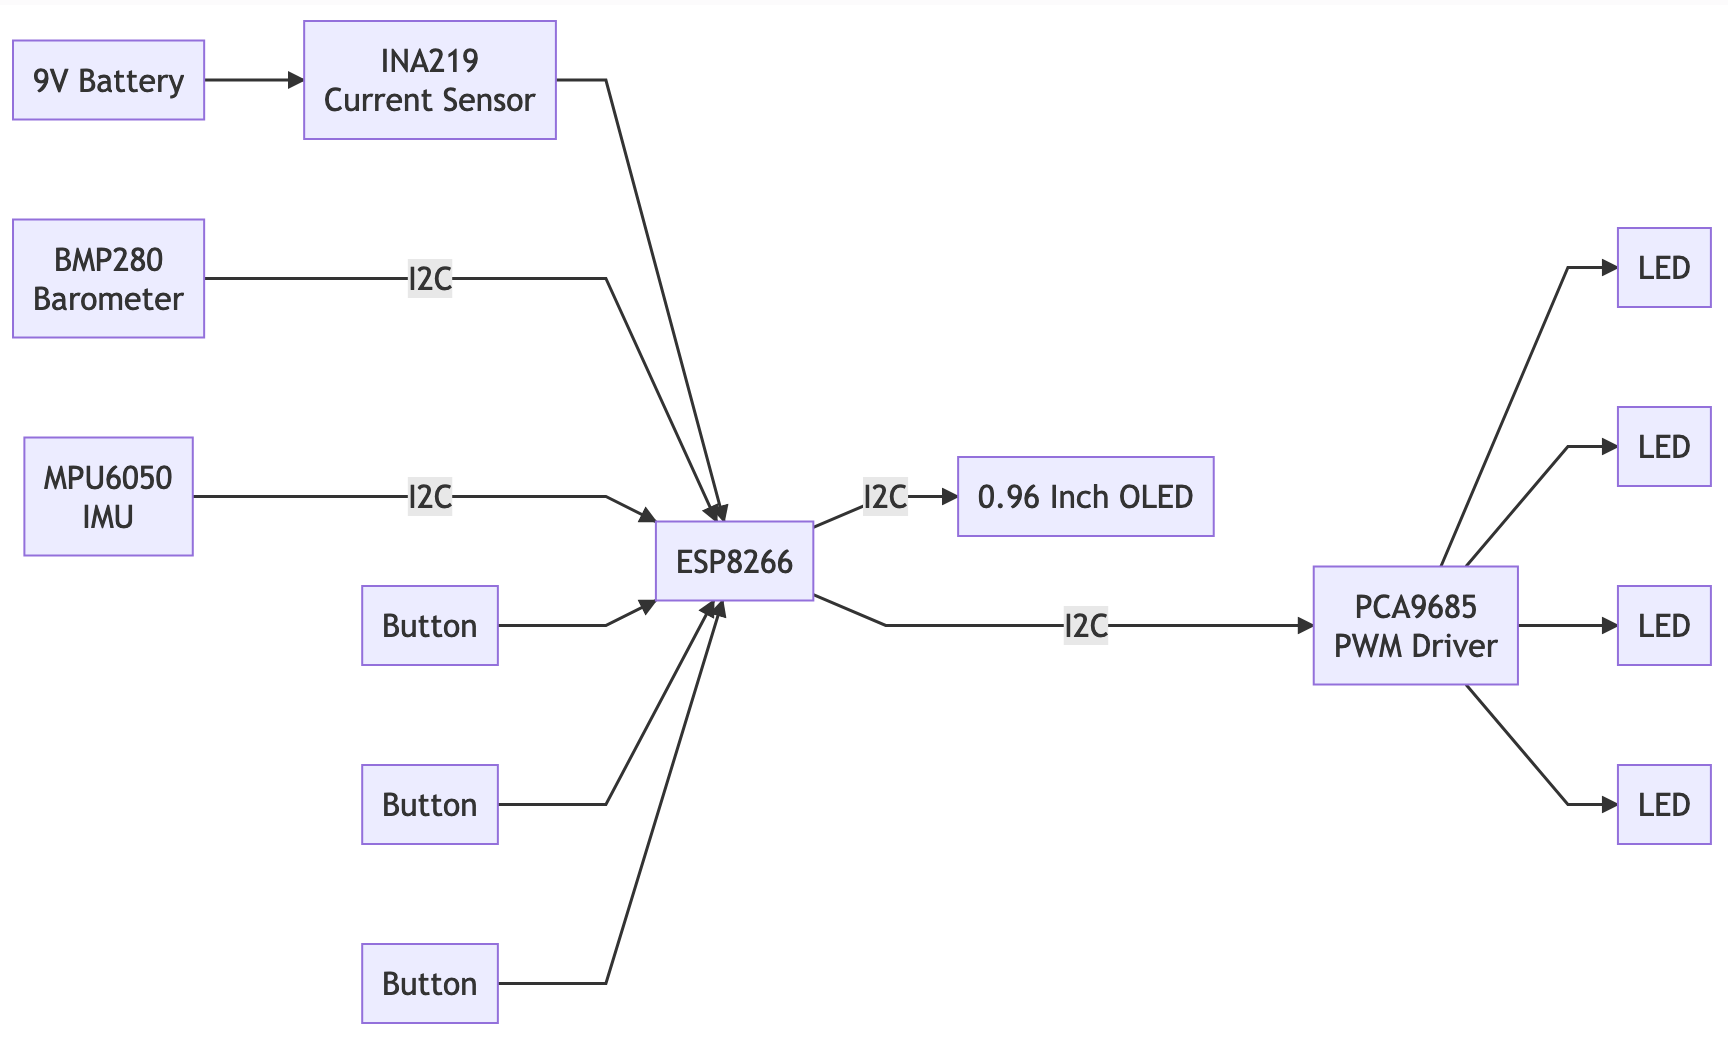
\includegraphics[width=0.4\textwidth]{images/final_design_prototype.png}
    \caption{Block diagram for the hardware demonstration of the project}
    \label{fig:final_design_prototype}
    
% graph LR
%   battery[9V Battery] --> curr
%   curr[INA219 <br> Current Sensor] --> esp[ESP8266]
%   baro[BMP280 <br> Barometer] ---> |I2C| esp
%   imu[MPU6050 <br> IMU] ---> |I2C| esp

%   esp ---> |I2C| pwm[PCA9685 <br> PWM Driver]
%   pwm --> led1[LED]
%   pwm --> led2[LED]
%   pwm --> led3[LED]
%   pwm --> led4[LED]

%   button1[Button] --> esp
%   button2[Button] --> esp
%   button3[Button] --> esp
  
%   esp --> |I2C| oled[0.96 Inch OLED]
\end{figure}


%%%%%%%%%%%%%%%%%%%%%%%%%%%%%%%%%%%%%%%%%%%%%%%%%%%%%%%
\subsubsection{Consensus Algorithm and Networking}
The final design is expected to rely upon painlessMesh and the Raft consensus algorithm. We will use painlessMesh as the mesh networking library to relay the election and log replication messages among the nodes. For clarity, we split both these flows into two figures.

Figure \ref{fig:flow} shows the logical flow of the firmware running on each node. All of the nodes in the network will initialize a mesh network using painlessMesh and then switch to the follower state. Following the Raft algorithm, a leader node will be selected through an election process. Any new nodes will autonomously be added to the network by the painlessMesh library and will default to follower mode until they declare candidacy.

\begin{figure}[H]
    \centering
    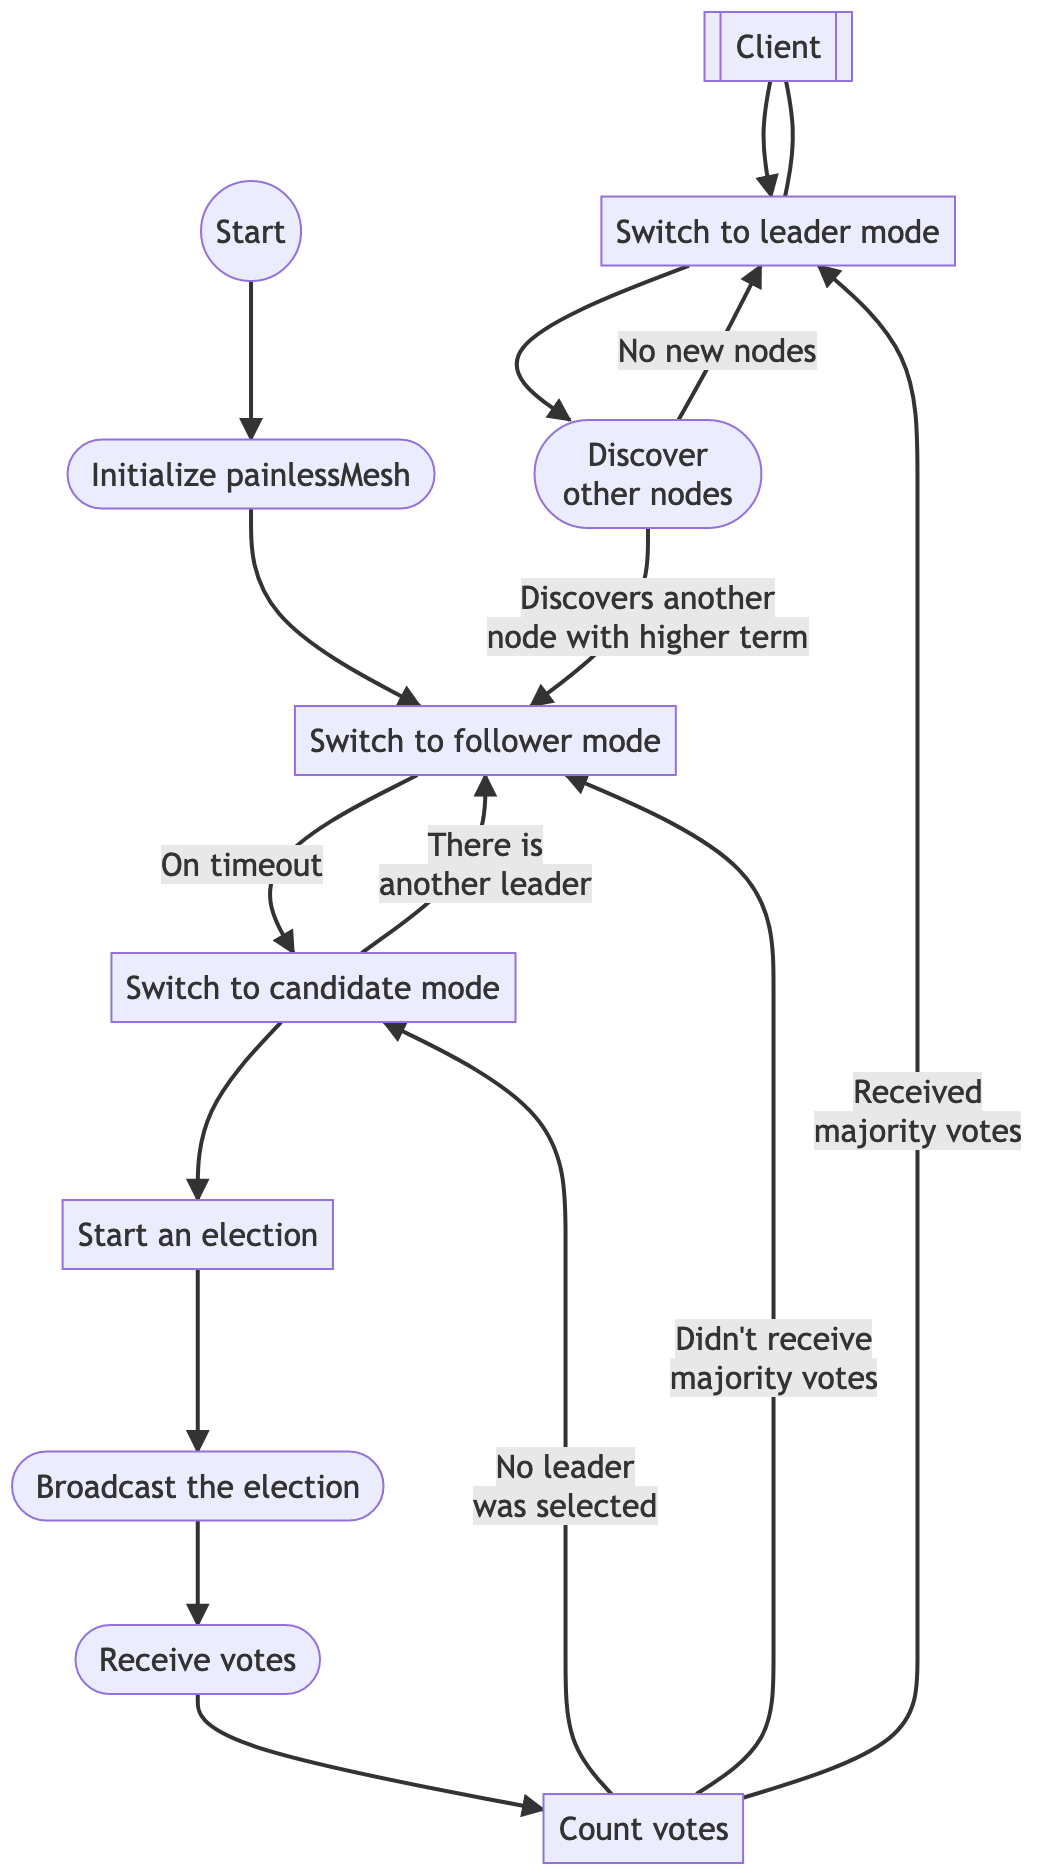
\includegraphics[width=0.58\textwidth]{images/final_design.png}
    \caption{Software logic}
    \label{fig:flow}

% flowchart TD
%   client[[Client]]
%   start((Start))

%   init([Initialize painlessMesh])
%   broadcast([Broadcast the election])
%   receive([Receive votes])
%   discover([Discover <br> other nodes])

%   follower[Switch to follower mode]
%   elect[Start an election]
%   candidate[Switch to candidate mode]
%   leader[Switch to leader mode]
%   count[Count votes]

%   start --> init
%   init --> follower
%   follower --> |On timeout| candidate
%   candidate --> elect
%   candidate --> |There is <br>another leader| follower
%   elect --> broadcast
%   broadcast --> receive
%   receive --> count
%   count --> |No leader <br> was selected| candidate
%   count --> |Didn't receive <br> majority votes| follower
%   count --> |Received <br>majority votes| leader

%   leader --> discover
%   discover --> |No new nodes| leader
%   discover --> |Discovers another <br> node with higher term| follower

%   client --> leader
%   leader --> client
\end{figure}

Figure \ref{fig:data_flow} shows three nodes replicating the logs to achieve consensus. Since Raft's primary goal is to achieve data consensus, we see that the leader node waits for confirmation whenever it communicates a change in data to a follower node. Once again, we will use the broadcast capabilities of the painlessMesh networking library to communicate between nodes as well as store the data received from communication onto the device's local storage. This data replication occurs in conjunction with the leader election process.

\begin{figure}[H]
    \centering
    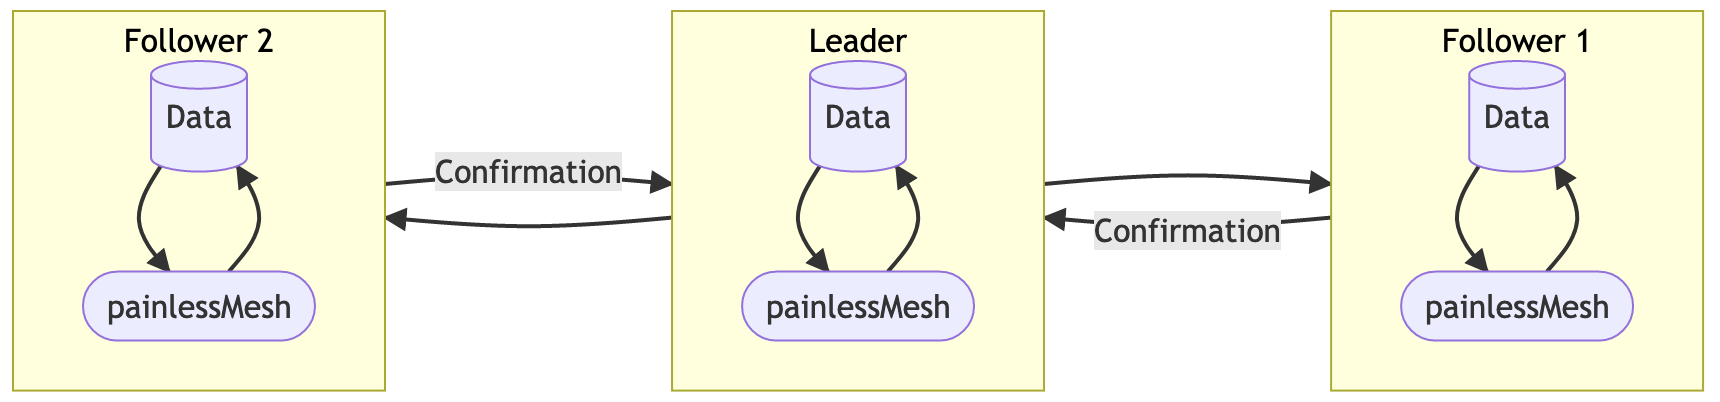
\includegraphics[width=0.8\textwidth]{images/final_design_data.png}
    \caption{Data flow between leader and follower nodes}
    \label{fig:data_flow}
\end{figure}

\subsection{Changes Made to Initial Design}

The changes to our design all stem from updates and improvements to our understanding of how to implement the software library. To concretize our design, we laid out our software library in a Unified Modeling Language (UML) diagram (Figure \ref{fig:uml}. We envision the software library to be broken down into three modules: the server, the data log, and the data queue. The server handles all the communication to achieve data consensus and interfaces with the data log and data queues. Further discussion regarding the "data log" can be found in Section \ref{sub:changes_made}. The data log is the data storage unit where each node stores data shared by the consensus leader. The data queue is a buffer where the client adds data to be sent to the leader.

\begin{figure}[H]
    \centering
    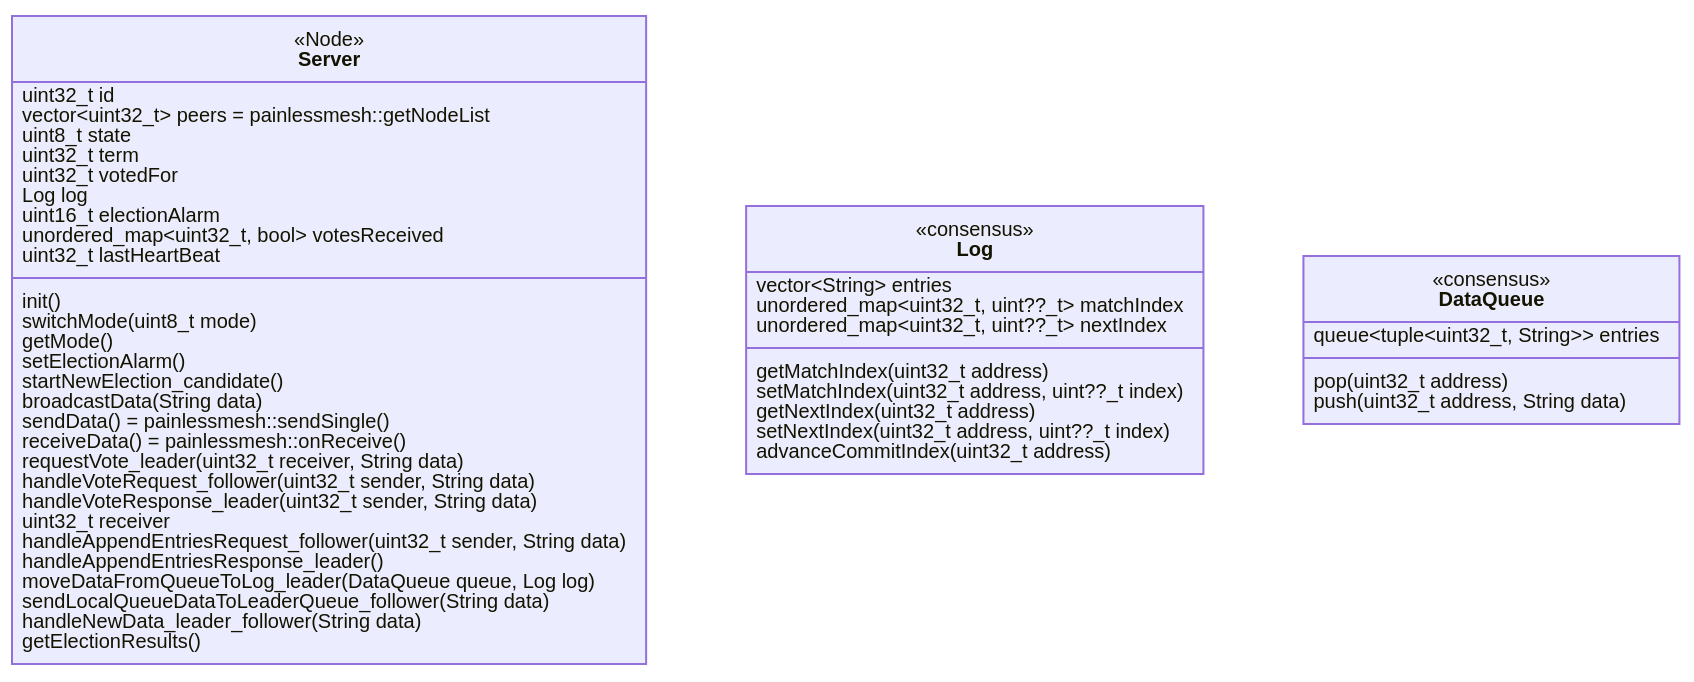
\includegraphics[width=\textwidth]{images/uml.png}
    \caption{UML diagram for the software library}
    \label{fig:uml}
\end{figure}

We updated a few components on the PCB due to better availability and documentation. Specifically, we updated the barometer to select the LPS25HB over the BMP280 and the I2C PWM driver to be PCA9635 instead of the PCA9685. After updating the components, we designed the schematic and routed the PCB as seen in Figures \ref{fig:pcb_schematic} and \ref{fig:pcb}.

\begin{figure}[H]
   \centering
   \begin{tabular}{@{}c@{\hspace{.5cm}}c@{}}
       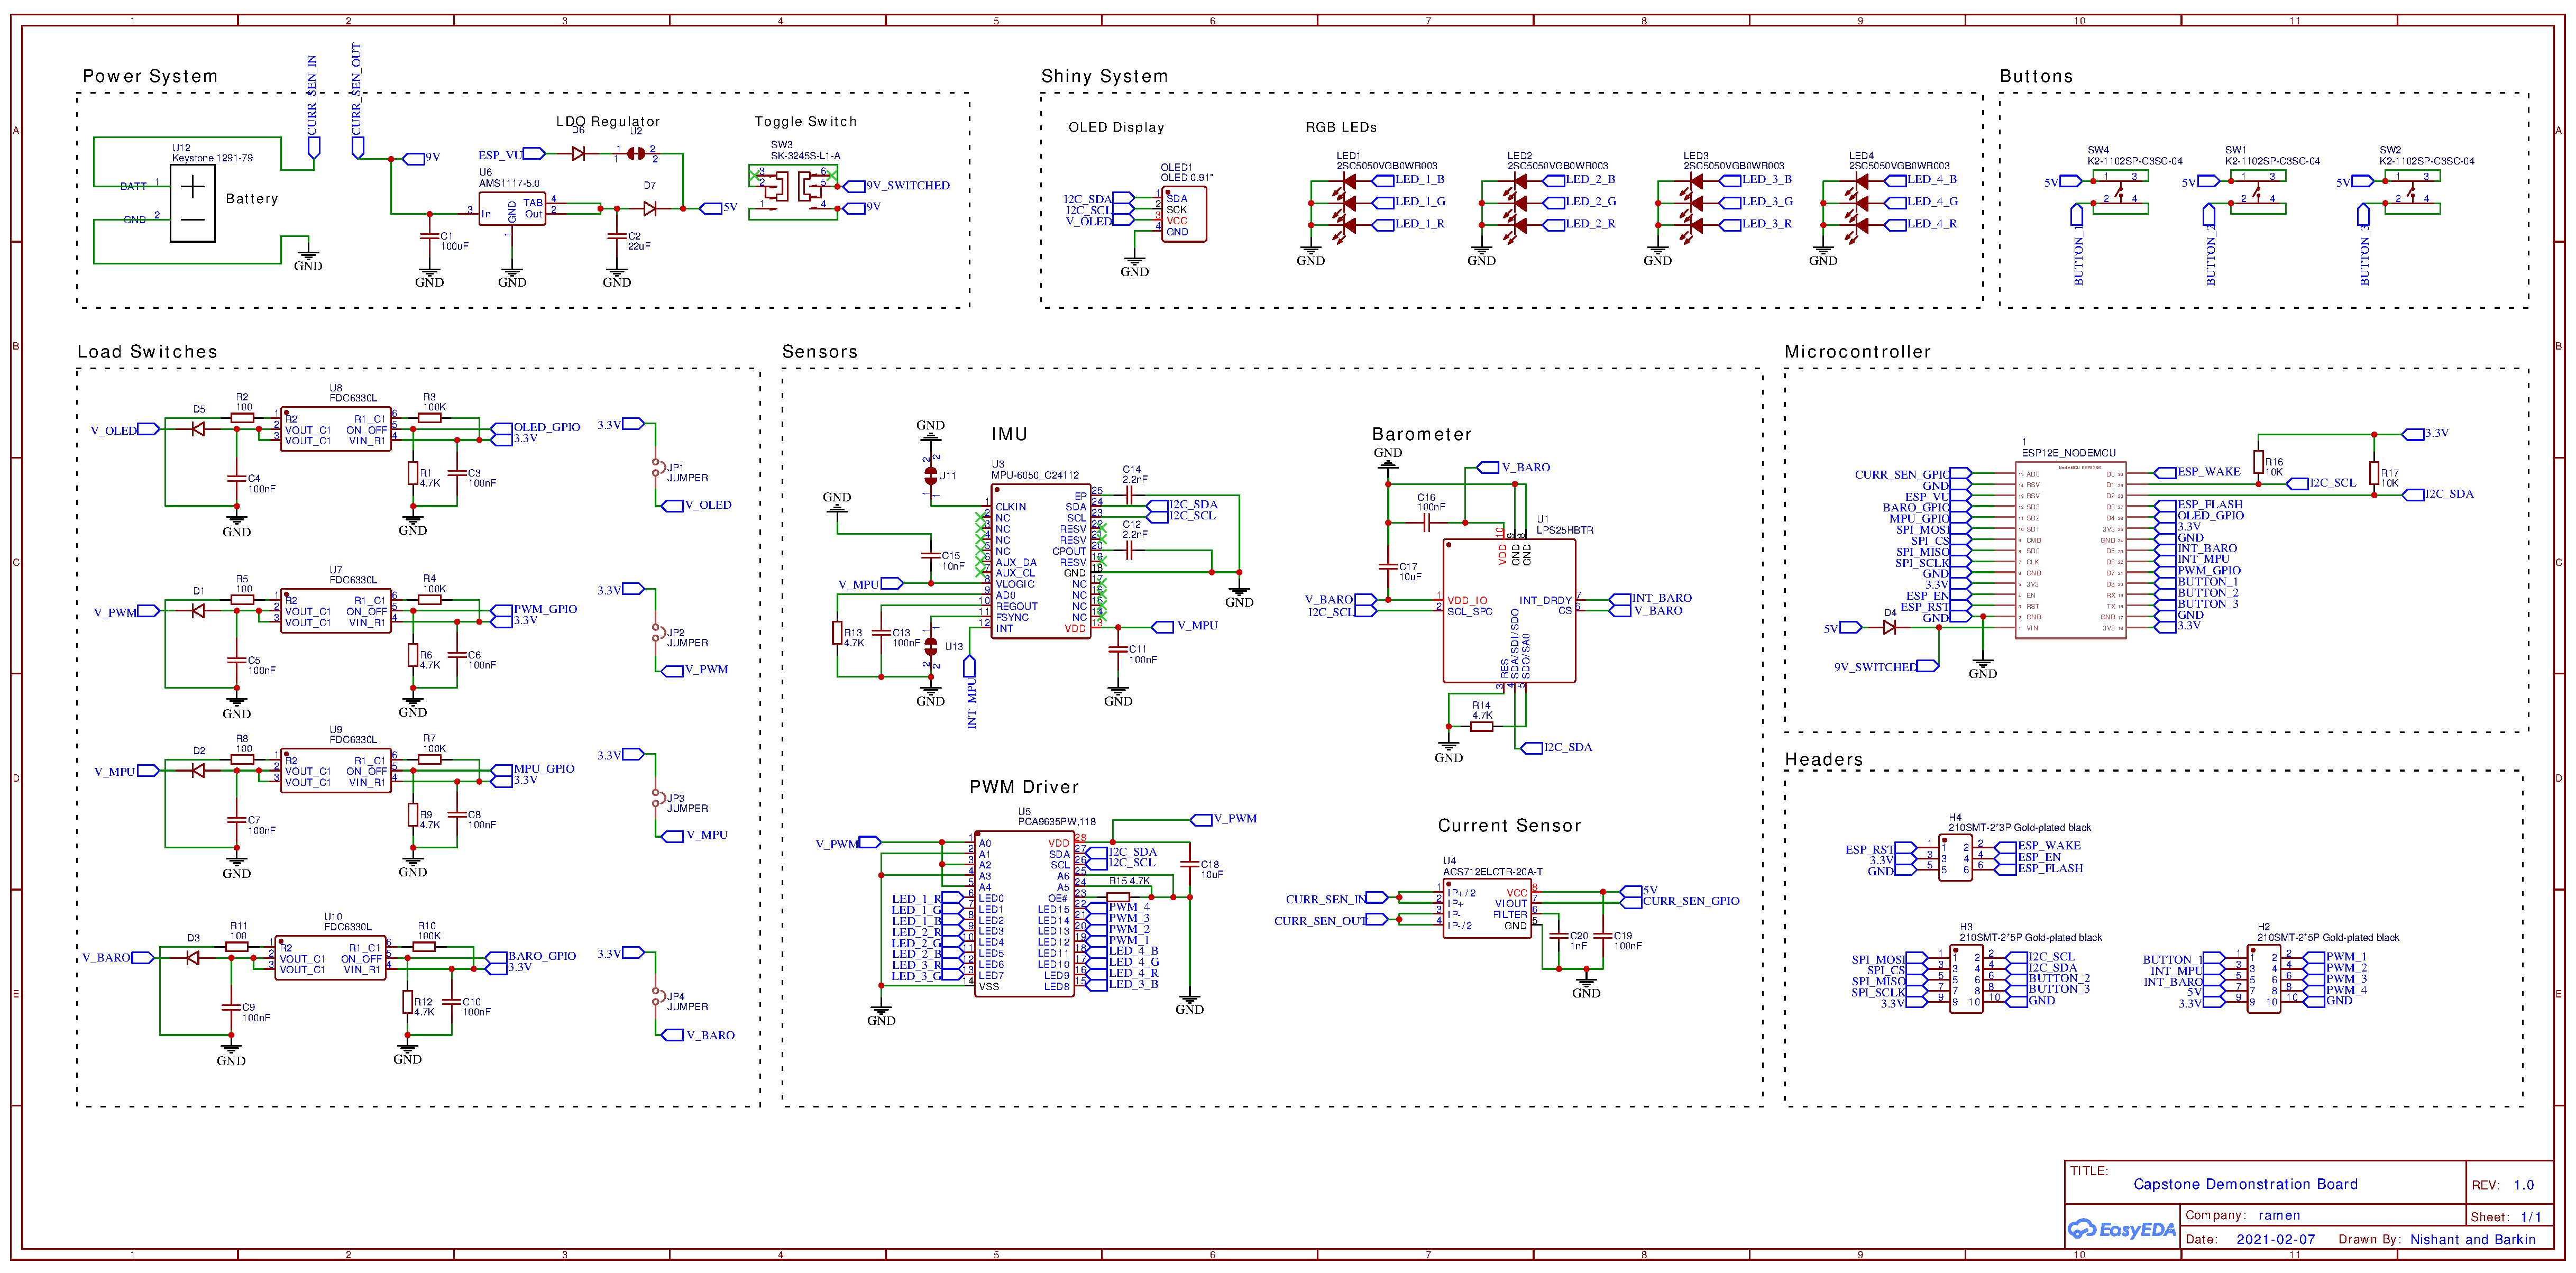
\includegraphics[page=1,width=1\textwidth]{images/pcb_schematic.pdf} \\
   \end{tabular}
 \caption{Designed PCB schematic}
 \label{fig:pcb_schematic}
\end{figure}


\begin{figure}[H]
    \centering
    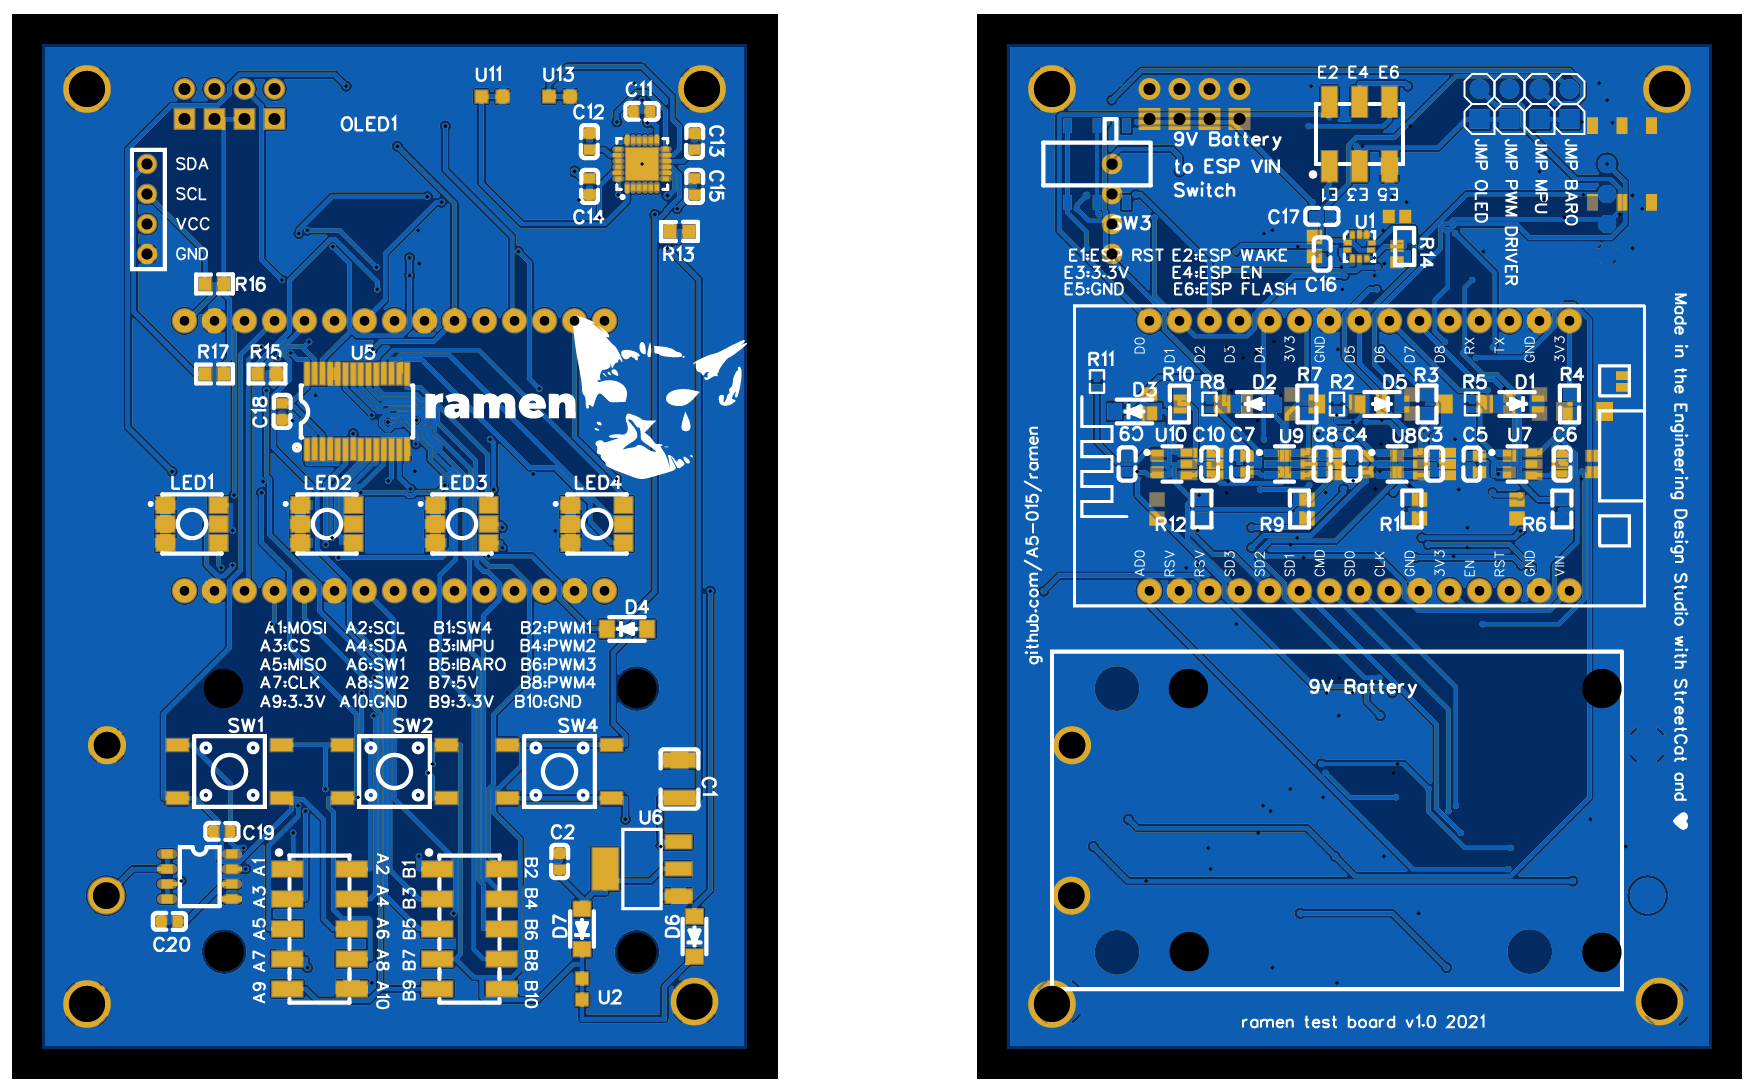
\includegraphics[width=0.45\textwidth]{images/pcb.png}
    \caption{Designed PCB}
    \label{fig:pcb}
\end{figure}


% flowchart LR
%   subgraph Leader
%     data[(Data)]
%     painlessMesh([painlessMesh])
%     data --> painlessMesh --> data
%   end

%   subgraph Follower_1[Follower 1]
%     f_1_data[(Data)]
%     f_1_painlessMesh([painlessMesh])
%     f_1_data --> f_1_painlessMesh --> f_1_data
%   end

%   subgraph Follower_2[Follower 2]
%     f_2_data[(Data)]
%     f_2_painlessMesh([painlessMesh])
%     f_2_data --> f_2_painlessMesh --> f_2_data
%   end
  
%   Leader --> Follower_2
%   Leader --> Follower_1
%   Follower_1 --> |Confirmation| Leader
%   Follower_2 --> |Confirmation| Leader




 
 

%%%%%%% BILL OF MATERIALS %%%%%%%
% No new page
\section{Budget and Bill of Materials}

% Since our project is mainly focused on producing a software library, we have a limited number of materials and hardware to procure. 
The required items for the demonstration of the software library and can be found in Table \ref{tab:bill_of_materials}.

\begin{table}[H]
    \scriptsize
    \centering
    \renewcommand{\arraystretch}{1.3}
    \vspace{10pt}
    \caption{Bill of materials required to build the hardware demonstration}
    \label{tab:bill_of_materials}
    \begin{tabular}{|c|c|c|c|c|c|}
        \hline
        \textbf{No} &
        \textbf{Part} &
        \textbf{Webpage} &
        \textbf{Unit Price (\$)} & 
        \textbf{Quantity} &
        \textbf{Total Price (\$)} \\
        \thickhline 
        1  & ESP8266 (NodeMCU Lolin V3) & https://www.aliexpress.com/item/32665100123.html & 2.13 & 15 & 31.95 \\
        \hline
        2 & PCB Prototype & https://www.pcbway.com & 0.49 & 20 & 9.80 \\
        \hline
        3 & 3D Printed Case & https://www.shapeways.com/ & 10 & 15 & 150 \\
        \hline
        4 & 9V Battery & https://amazon.ae/Duracell-32059-9V-Batteries-pieces/dp/B0014D0SL8 & 3.68 & 15 & 55.2 \\
        \hline
        5 & BMP280 Barometer & https://www.aliexpress.com/item/32950712562.html & 0.27 & 15 & 4.05 \\
        \hline
        6 & MPU6050 IMU & https://www.aliexpress.com/item/1005001724323744.html & 0.41 & 15 & 6.15 \\
        \hline
        7 & 4.1 MM 5V Push button & https://www.aliexpress.com/item/1058764733.html & 0.02 & 60 & 1.2 \\
        \hline
        8 & RGB SMD LED 3528 & https://www.aliexpress.com/item/32384196929.html & 0.003 & 60 & 0.18 \\
        \hline
        9 & PCA9635 PWM Driver & https://www.aliexpress.com/item/4001111573844.html & 1.20 & 15 & 18 \\
        \hline
        10 & 0.96 Inch OLED Display & https://www.aliexpress.com/item/1005001564950878.html & 1.10 & 15 & 16.5 \\
        \hline
        11 & Shipping and Bank Fees &  & 47.97 & 1 & 16.5 \\
        \hline
        \multicolumn{5}{|r|}{Grand Total (\$)} & 341 \\
        \hline
    \end{tabular}
\end{table}

%%%%%%% IMPLEMENTATION DETAILS %%%%%%%
\newpage
\section{Implementation Details}

\subsection{Implementation Successes}
We found that the general flowchart (see Figure \ref{fig:data_flow}) we had designed for implementing the software library was accurate. Hence, during each work session, we were able to identify modules of the Raft consensus algorithm from our flowchart and successfully implement these modules using the API exposed to us by the painlessMesh software library. The following is a list of our successes in attempting to implement Raft atop painlessMesh:

\begin{itemize}
  \item Designing a UML diagram (see Figure \ref{fig:uml}) to document and build a detailed architecture of our software library.
  \item Setting up a PlatformIO (PIO) project capable of uploading and managing the ESP devices being tested. This PIO project will also be useful for eventual end-users to rapidly install and work with our software library.
  \item Implementing a virtual testing framework (see Figure \ref{fig:virtual_ramen}) that mimics painlessMesh and interacts with our library to simulate a large number of nodes for debugging and scale-testing purposes.
  \item Completing the initialization, voting communication, state switching, and leader selection modules of the Raft consensus algorithm.
  \item Designing a portable PCB (as specified in Figure \ref{fig:final_design_prototype}) with an ESP8266 chip, various sensors, an onboard battery case that will allow us to conduct scale and distance tests for our software library. The completed schematic and PCB designs can be seen in Figures \ref{fig:pcb_schematic}, \ref{fig:pcb}, and \ref{fig:ramen_photo}.
\end{itemize}

\begin{figure}[H]
    \centering
    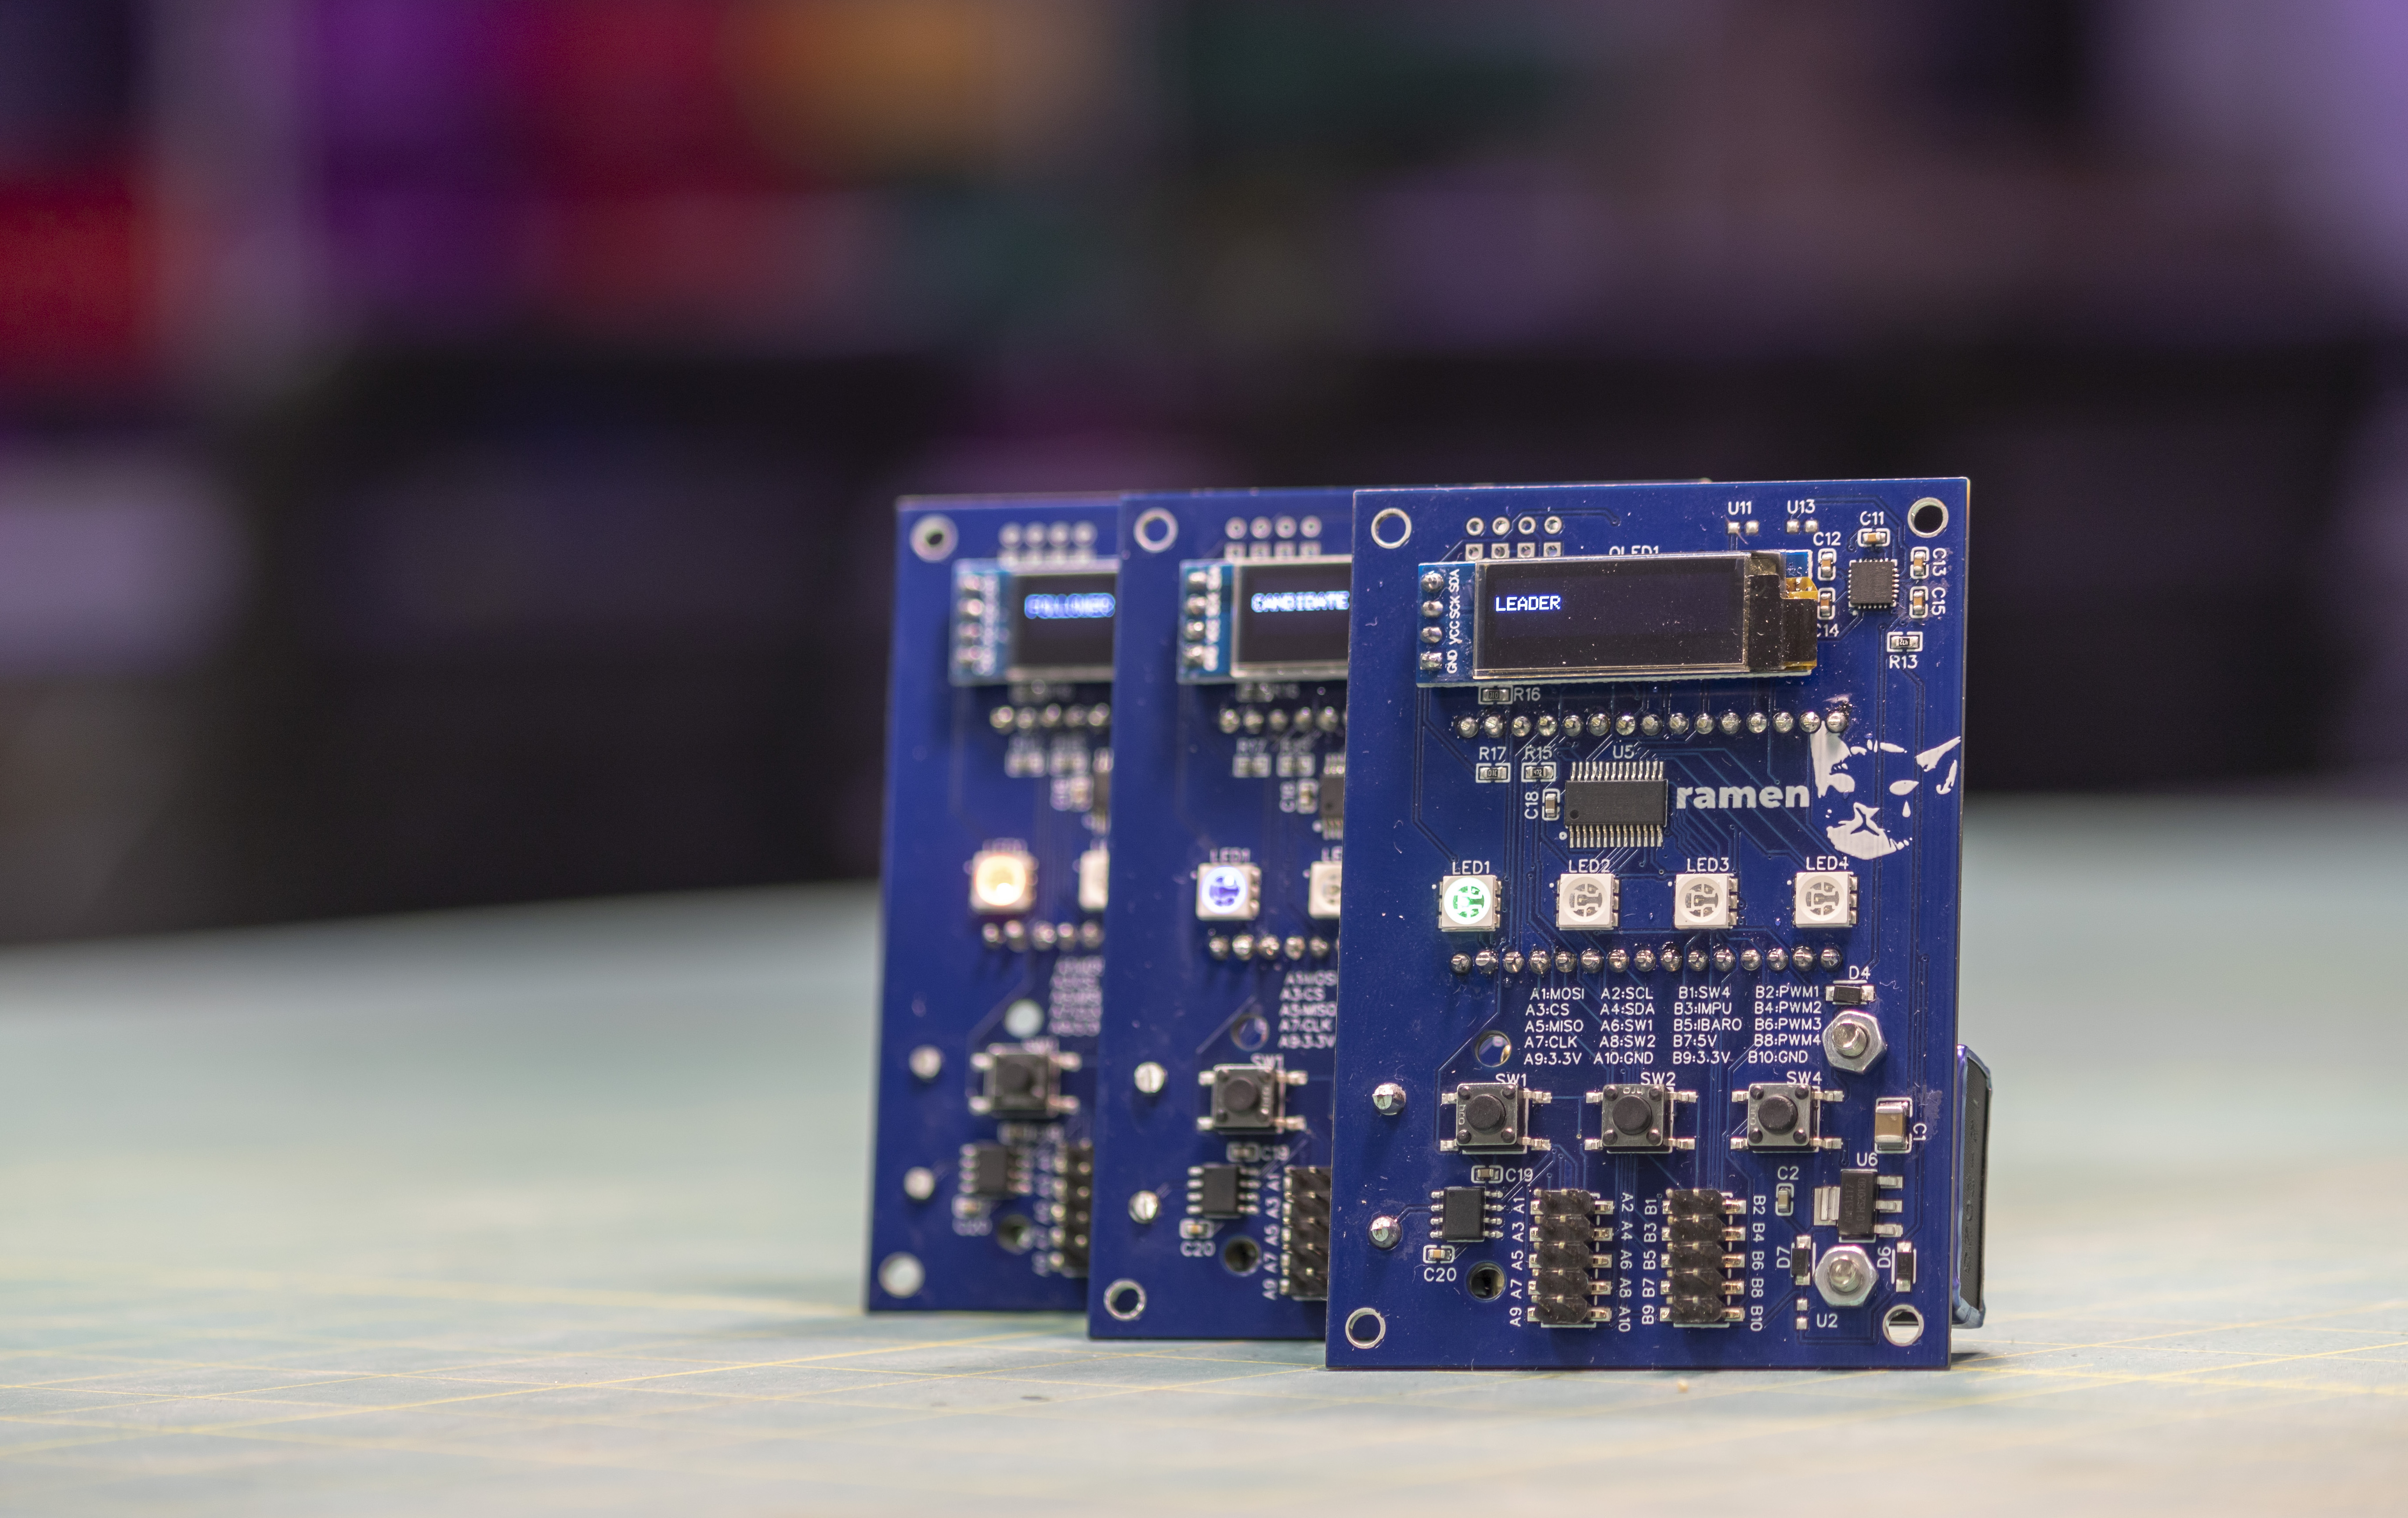
\includegraphics[width=0.84\textwidth]{images/ramen_photo.jpg}
    \caption{Custom designed PCBs running our software library}
    \label{fig:ramen_photo}
\end{figure}

In order to enhance our software library and improve overall reliability, we suggest the following:

\begin{itemize}
  \item Add acknowledgment (ACK) and negative acknowledgment (NACK) packets to the log messages sent between nodes.
  \item Decrease the amount of time it takes for the network to realize that a node has been disconnected.
  \item Dynamically update the log broadcast frequency of the leader based on network conditions, such as communication latency.
  \item Allow end users to broadcast multiple messages to the network at once.
  \item Allow end users to broadcast messages of various data types (integers, floats, booleans) beyond strings.
\end{itemize}


\subsection{Issues Faced}
We did not come across any significant challenges when building our software library. The notable challenges we came across were a result of a mismatch between our flowchart and UML diagram against the Raft paper \cite{raft_paper}. Hence, during our work sessions, we returned back to the Raft consensus algorithm and better understood the details so that we could accurately implement these details in our software library. This involved us updating the flowchart and UML diagram to align with the framework outlined in the Raft consensus algorithm paper.

Every bug we encountered involving unexpected behavior was quickly identified by referencing our log messages and finding anomalies in our virtual testing framework. Then, the fixed behavior was compared against the interactive browser implementation of Raft \cite{raft_website} to ensure accurate implementation. 

\subsection{Changes Made}
\label{sub:changes_made}
The Raft consensus algorithm accounts for multiple clients on the network attempting to pass data onto the servers. Specifically, the Raft paper states that "if a client contacts a follower, the follower redirects it to the leader" \cite{raft_paper}. However, this situation assumes a network where clients have direct access to the leader. In the case of a network of embedded devices, we consider the "clients" to be the sensors on each node. Hence, these "clients" do not have direct access to the leader. As a result, we slightly modify the Raft algorithm to account for such scenarios. 

We envision each follower node to have a client associated with it. In our suggested modification, these clients, when seeking to add data to the network's logs, are not redirected to the network's leader node. Rather, they add their data to the server's data buffer. At each time interval, the follower node checks its data buffer to forward these messages to the leader node's data buffer. Similarly, the leader node periodically checks its data buffer for such messages, which are then pushed into the network using the Raft algorithm. 

Our modification remains true to the operation of the Raft consensus algorithm in that follower nodes are not allowed to push data into the network. We simply provide an alternative implementation given that most clients on the network cannot directly access the leader node. 

\subsection{Initial Results}

Section \ref{sec:coracle_results} describes the results we obtained from Coracle simulations to compare mesh and star networks, as well as the performance of mesh networks as the Raft parameters are varied.

As we describe in Section \ref{sec:virtual_mesh_simulation}, we also developed a virtual mesh network simulation to test and execute our Raft implementation. The virtual simulation is capable of creating hundreds of virtual boards for testing our code. This scale of software testing would not be possible on real hardware due to budget and time constraints. Thus, the virtual testing framework lets us rapidly test our code and debug when needed.

Figure \ref{fig:virtual_ramen} shows a virtual network of 3 nodes running the initial version of our software library. When we look at the log messages outputted by each node, we see that \texemphtit{node 1} starts an election and requests votes from the other nodes. Later, \emph{nodes 2} and \emph{3} grants vote to \emph{node 1} during the election. As a result, \emph{node 1} becomes the leader in Raft consensus.

\vspace{-15pt}

\begin{figure}[H]
    \centering
    \subfloat{{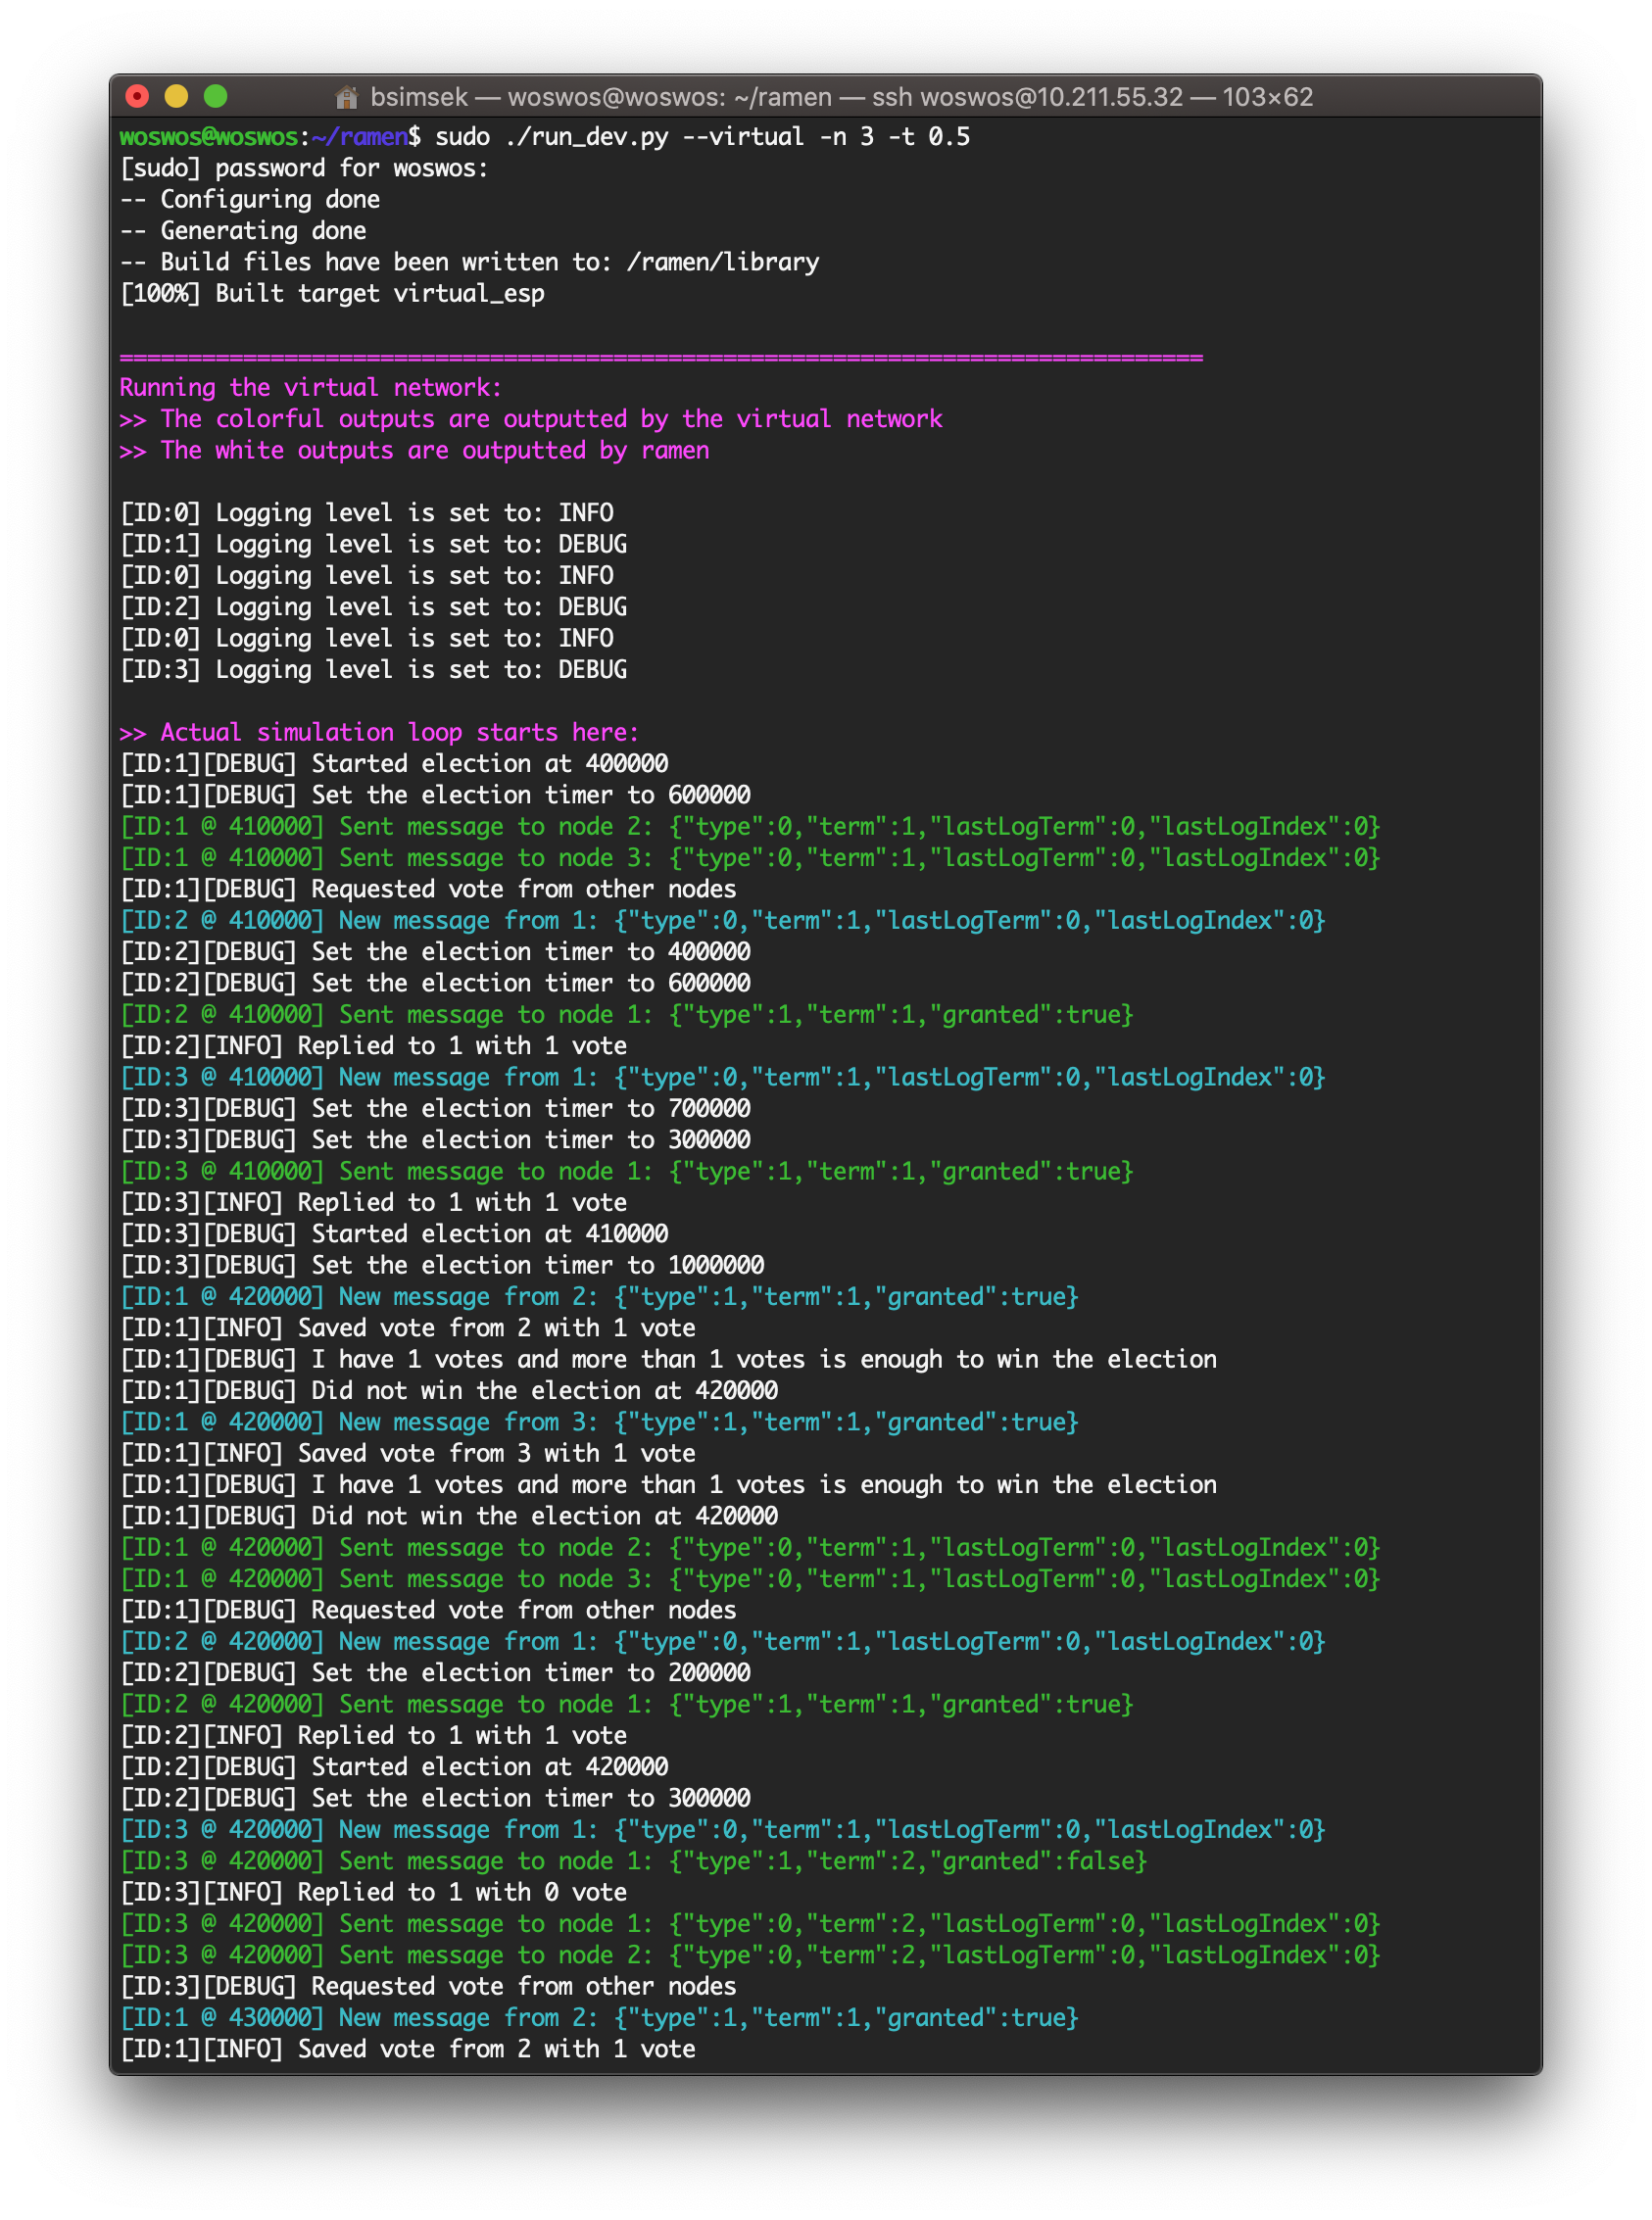
\includegraphics[width=0.44\columnwidth]{images/virtual_ramen_1.png} }}%
    \qquad
    \subfloat{{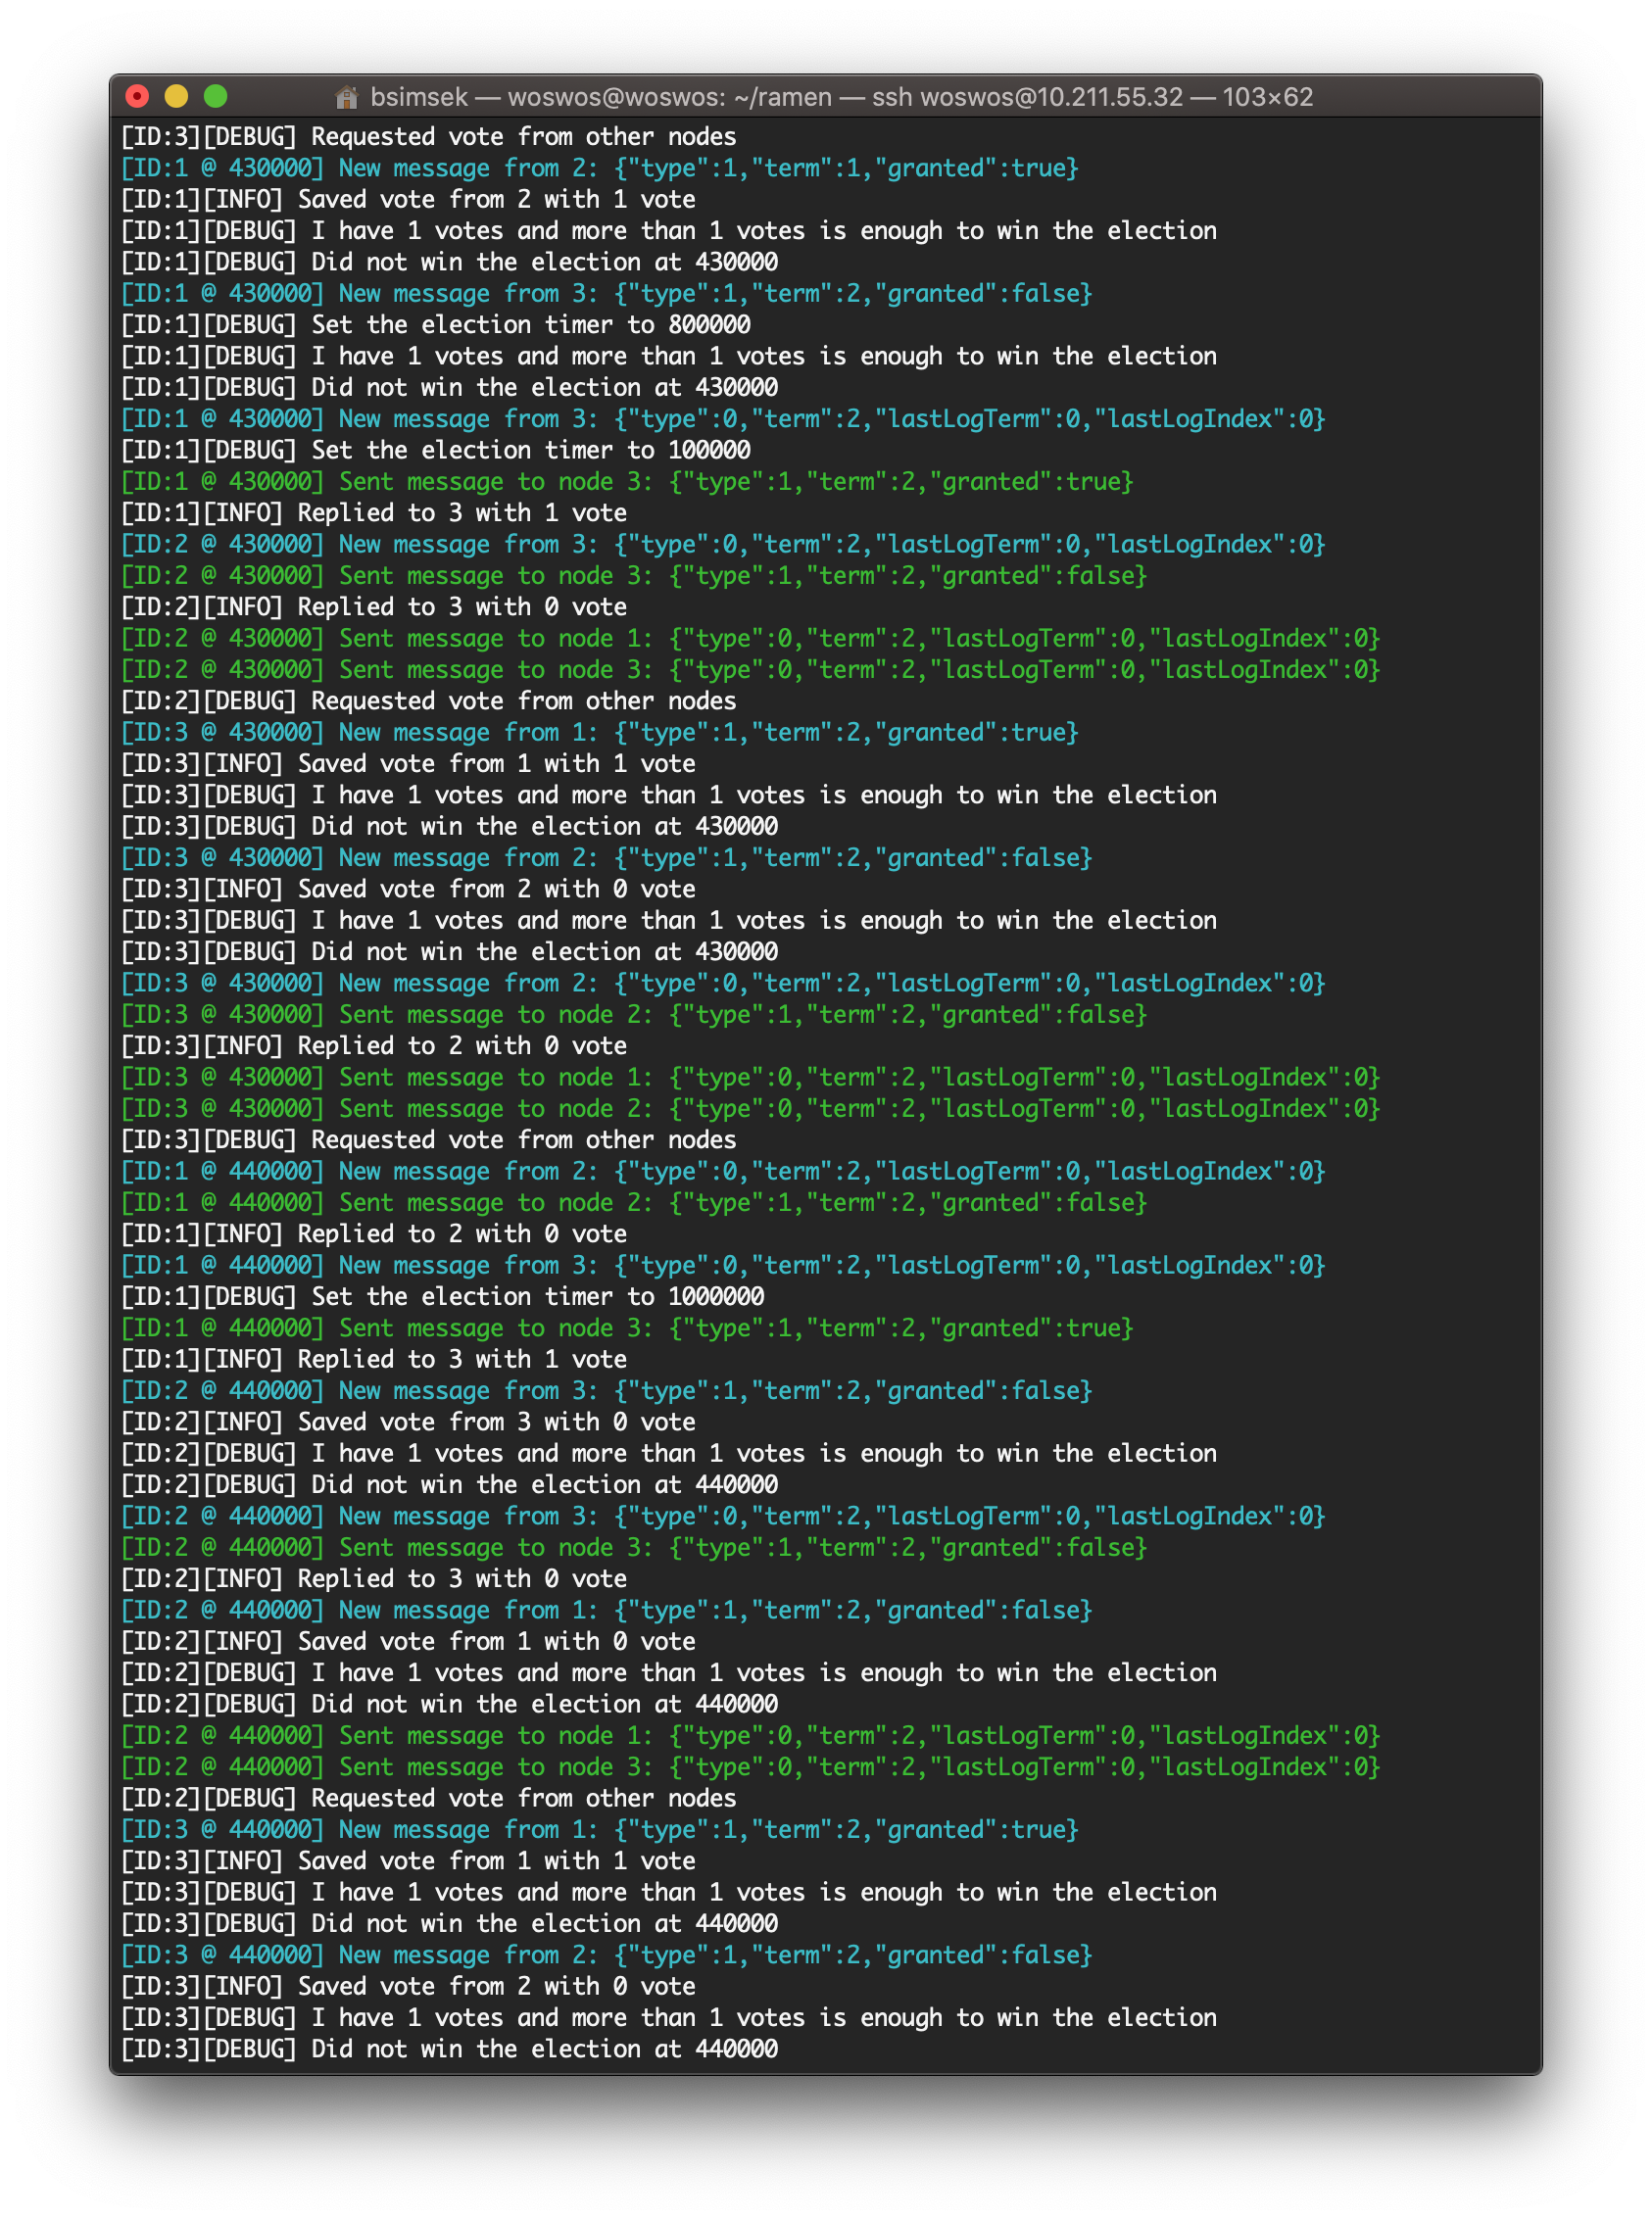
\includegraphics[width=0.44\columnwidth]{images/virtual_ramen_2.png}}}%
    \caption{ramen software running in the virtual simulated mesh network environment. Read top to bottom, left to right.}
    \label{fig:virtual_ramen}%
    \medskip
\end{figure}

In addition to the virtual testing framework, we also tested the initial version on the physical boards we have and confirmed the functionality. However, using virtual testing saves us a significant amount of development and testing time.

%%%%%%% ETHICS %%%%%%%
\newpage
\section{Ethics}

\subsection{Applications and Use-cases}
Consensus algorithms on embedded systems are often used in critical scenarios, such as in the real-time control of multi-agent systems \cite{ConsensusClassDiscretetime, Olfati_Saber_Fax_Murray_2007}. However, they may also find applications in less time-critical scenarios such as charge scheduling in Unmanned Aerial Vehicle (UAVs) \cite{hassijaSchedulingDroneCharging2020}. Using a system unsuited for real-time response and minimal latency in critical applications may lead to catastrophic yet avoidable failures. In the ideally successful completion of this project, our software library will be published with a permissible license and be modular enough for various implementations. As a result, we have a responsibility to provide a comprehensive analysis of the capabilities of our tool. \textit{For this concern, we will outline the limitations of our system by providing the results of the tests we use to evaluate the library.}

\subsection{Hardware and E-waste}
We will be producing a Printed Circuit Board (PCB) to demonstrate our software library and its use on mobile nodes. However, there exists a valid concern of generating electronic waste by designing a board that will not be reused in the future. Designing circuit boards for short life spans is a wasteful activity that contributes to the unhealthy consumer relationship with electronics, where rapid turnover is encouraged due to affordability. \textit{For this concern, we will design a more general development board with the potential to be reused in future projects for prototyping and similar demonstration purposes.}

%%%%%%% CODES AND STANDARDS %%%%%%%
\section{Codes and Standards}

This project relies on two communication standards: the IEEE 802.11 wireless standard for inter-node communication and the I2C protocol for communication between integrated chips on the demonstration PCB.

 Specifically, the ESP8266 chip supports the IEEE 802.11B/G/N protocols \cite{espressif:esp8266}. The mesh networking library used in this project, painlessMesh, only supports IEEE 802.11B and IEEE 802.11G, with the latter being the default protocol \cite{painlessMesh:wifi_standard}. Using the IEEE 802.11G protocol on the ESP8266 requires a transmit power of approximately $\SI{17}{dBm}$ and communication occurs within the $\SI{2.4 - 2.5}{GHz}$ frequency range \cite{espressif:esp8266}. Section \ref{section:networking_protocols} further discusses the IEEE 802.11 protocol in comparison to other available communication protocols.

The demonstration PCB uses the I$^2$C protocol for communication between the microprocessor, the sensors, and the display modules. The I$^2$C protocol, developed by Philips Semiconductors, transmits data over a single SDA line and clocks the device communication over the SCL line. A single I$^2$C bus can theoretically communicate with up to 127 secondary devices, although this number changes in practice based on the data rate and communication distance \cite{i2c_overview}. The I$^2$C protocol satisfies the integrated chip communication requirements for the demonstration PCB.

%%%%%%% IMPACT OF COVID-19 ON THE PROJECT %%%%%%%
% No new page
\section{Impact of COVID-19 on the Project}

In accordance with COVID-19 guidelines, our team had limited access to lab spaces throughout the duration of the project. While this did not significantly impact the project, given its focus on software, it made access to hardware more difficult for testing purposes. Overall, little was changed due to the pandemic as the project timeline and scope were designed with the existing and potential restrictions in mind.

%%%%%%% DESIGN EVALUATION %%%%%%%
%% deliverables
%% evaluation testing
%% test data
%% discussion on testing data
\newpage
\section{Design Evaluation}

\subsection{Virtual Mesh Network Simulation}
\label{sec:virtual_mesh_simulation}

In addition to using the Coracle simulator, we also developed a virtual mesh network simulator that interfaces with our software implementation to run rapid simulations and obtain readable logs for debugging and testing. The simulator also enables us to deploy our library implementation code to a large number of nodes, such as 100+ nodes, in a few seconds without actually buying the required hardware.

Our simulator directly runs our library implementation code without any modifications. The simulator virtualizes required resources such as the network card, serial input/output, and other dependent software libraries in order to provide an identical environment to the ESP8266 microcontroller, as shown in Figure \ref{fig:virtual_esp_diagram}. The simulation loads our library implementation code to virtual nodes in the simulated environment and manages the networking between these virtual nodes. As a result, we are able to control which nodes connect to each other and simulate various network conditions such as missing links. We are also able to add or remove new virtual nodes to the system and observe how the entire network behaves.

Furthermore, the simulator allows us to reliably collect metrics about our software implementation and learn how they change depending on parameters, such as the number of nodes in the network.


\begin{figure}[H]
    \centering
    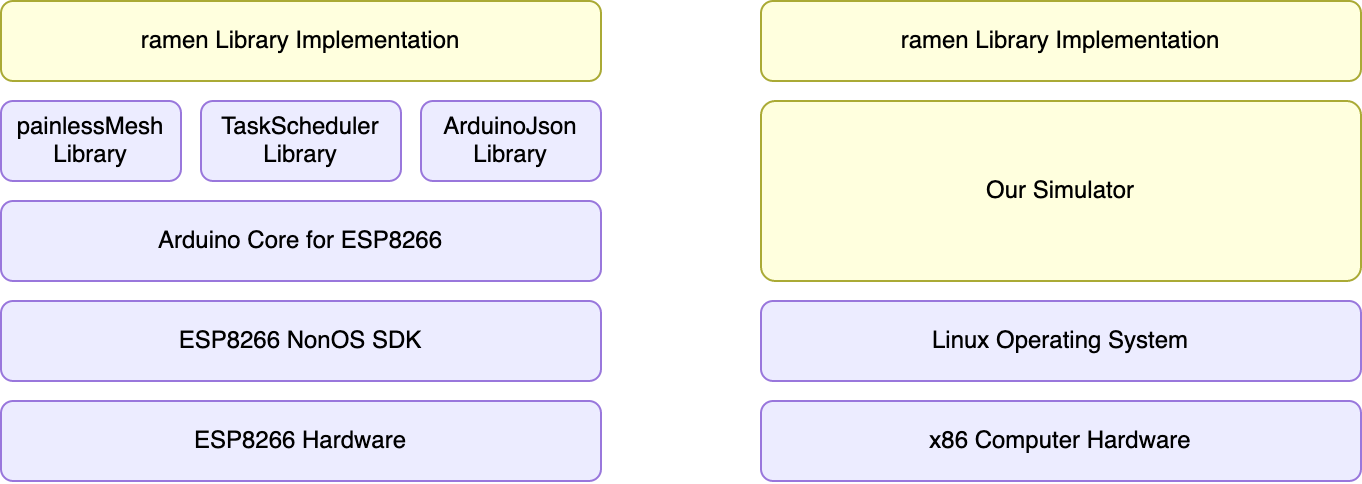
\includegraphics[width=0.85\columnwidth]{images/virtual_esp.png}
    \caption{Left: Our software implementation running on ESP8266 hardware, Right: Our software implementation running on our simulator }
    \label{fig:virtual_esp_diagram}
\end{figure}


\subsection{Criteria for Testing}

To evaluate our implementation of Raft, we have selected three main criteria: network scalability, network stability, and network realignment time. We first conducted experiments in the Coracle simulation to obtain a baseline. We then conducted the experiments in the virtual mesh simulation to test how our implementation compared.

\begin{itemize}
    \item \textit{Network scalability:}
    \begin{itemize}
        \item Network scalability refers to how well the network performs with various densities of nodes. Increasing the number of nodes should not significantly increase latency.
    \end{itemize}

    \item \textit{Network stability:}
    \begin{itemize}
        \item Network stability implies that the network should perform reliably and consistently over time so as to avoid any loss of data. 
    \end{itemize}
    
    \item \textit{Realignment time:}
    \begin{itemize}
        \item Realignment time measures the network's ability to recover from abrupt changes to the system, such as the loss of a leader.
    \end{itemize}
\end{itemize}



\subsection{Test Data}

Each simulation shown in Figures \ref{fig:virtual_vary_nodes}, \ref{fig:virtual_vary_duration}, \ref{fig:virtual_vary_heartbeat}, \ref{fig:virtual_vary_election_timeout}, and \ref{fig:virtual_vary_leader_kill} was run for 60 seconds in the virtual mesh network simulator using our ramen library. Each of the simulations shown in Figures \ref{fig:virtual_vary_duration}, \ref{fig:virtual_vary_heartbeat}, and \ref{fig:virtual_vary_election_timeout} were run with 5 nodes per run.

\subsubsection{Measurements}

\begin{figure}[H]
    \centering
    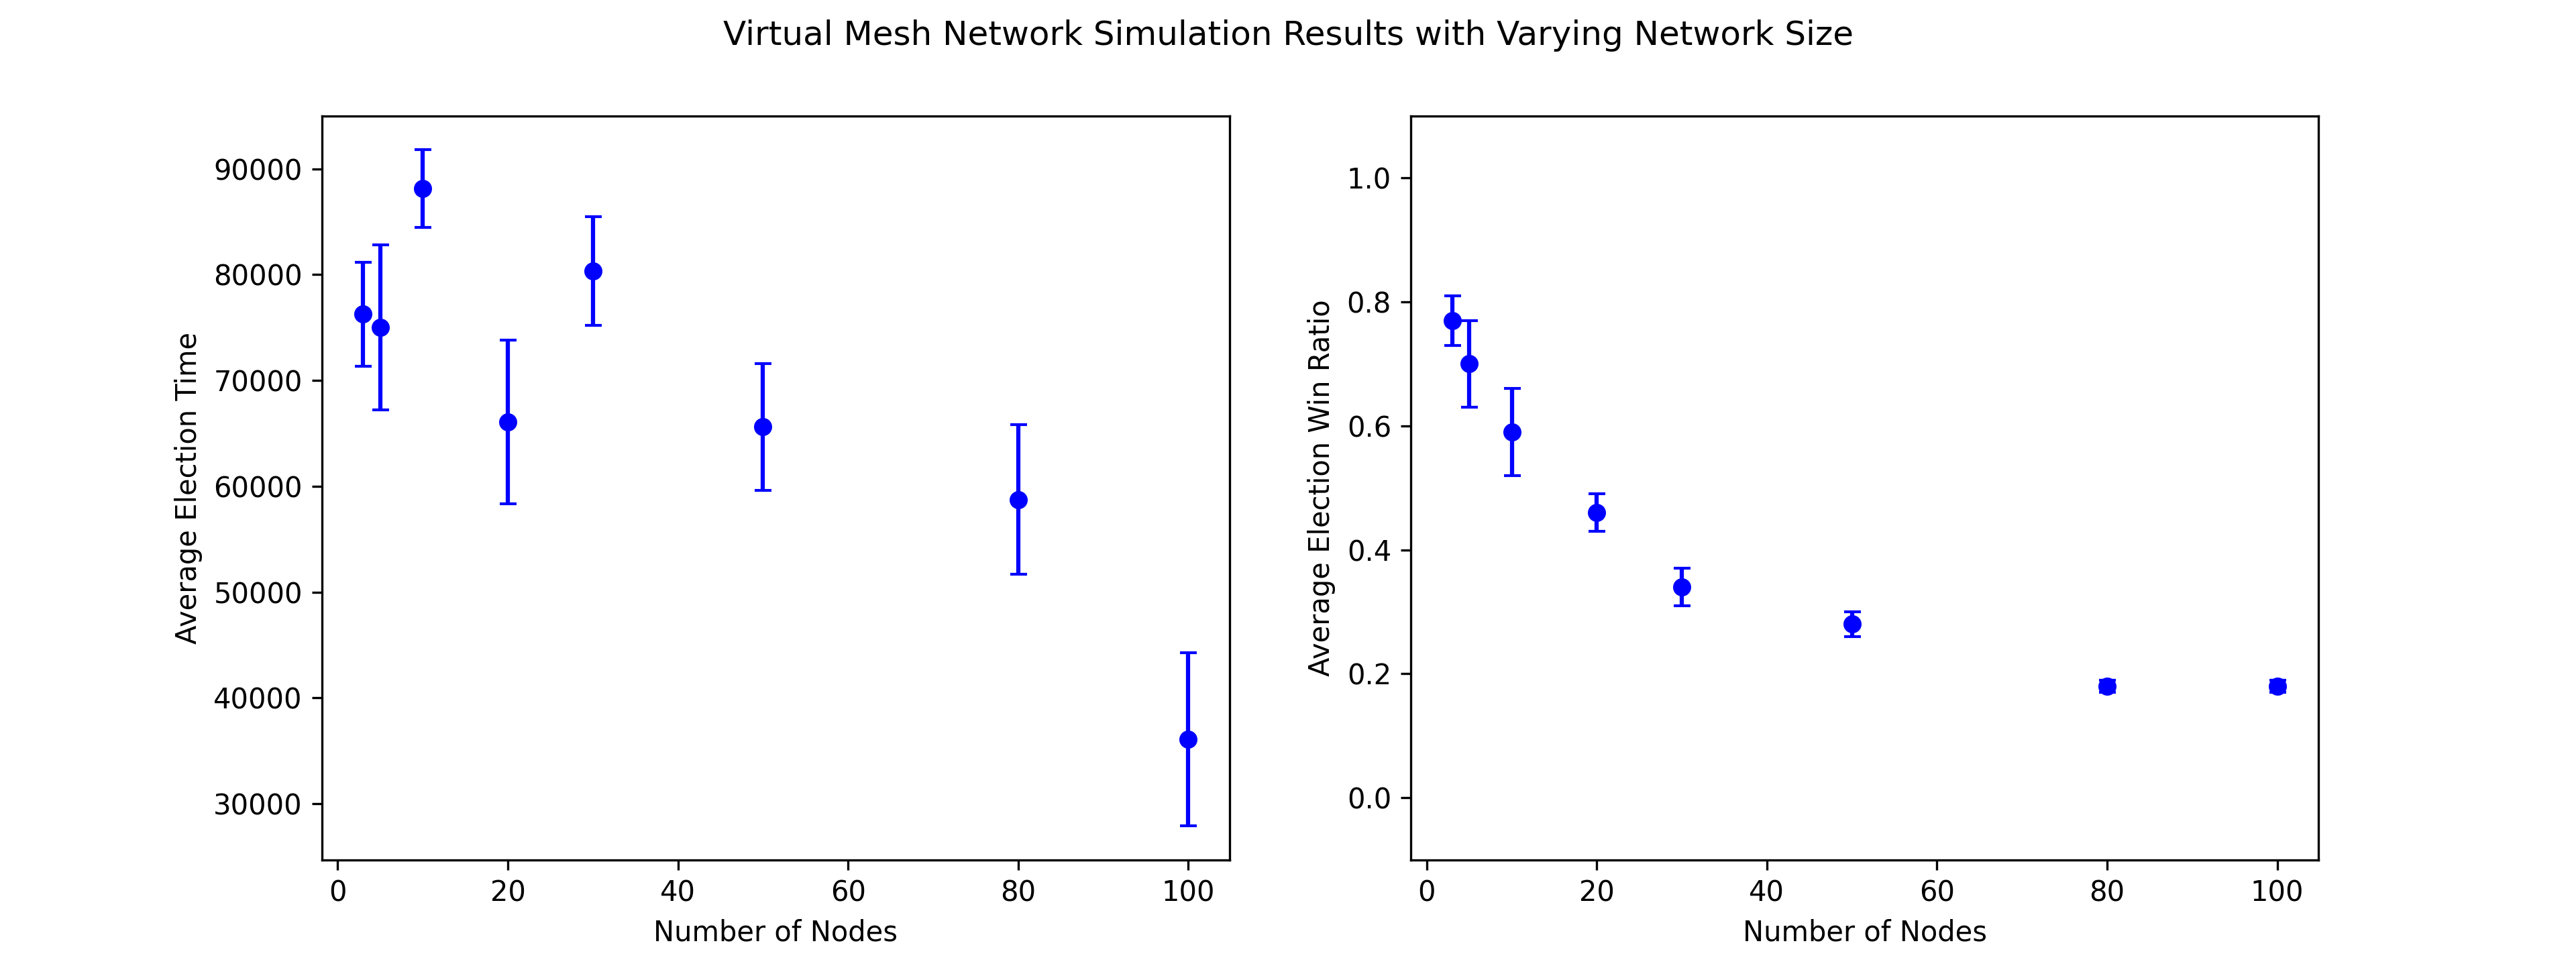
\includegraphics[width=0.9\columnwidth]{images/virtual_vary_nodes.png}
    \caption{Left: Average election time per number of nodes, Right: Average ratio of elections won to initiated per number of nodes}
    \label{fig:virtual_vary_nodes}
\end{figure}


\begin{figure}[H]
    \centering
    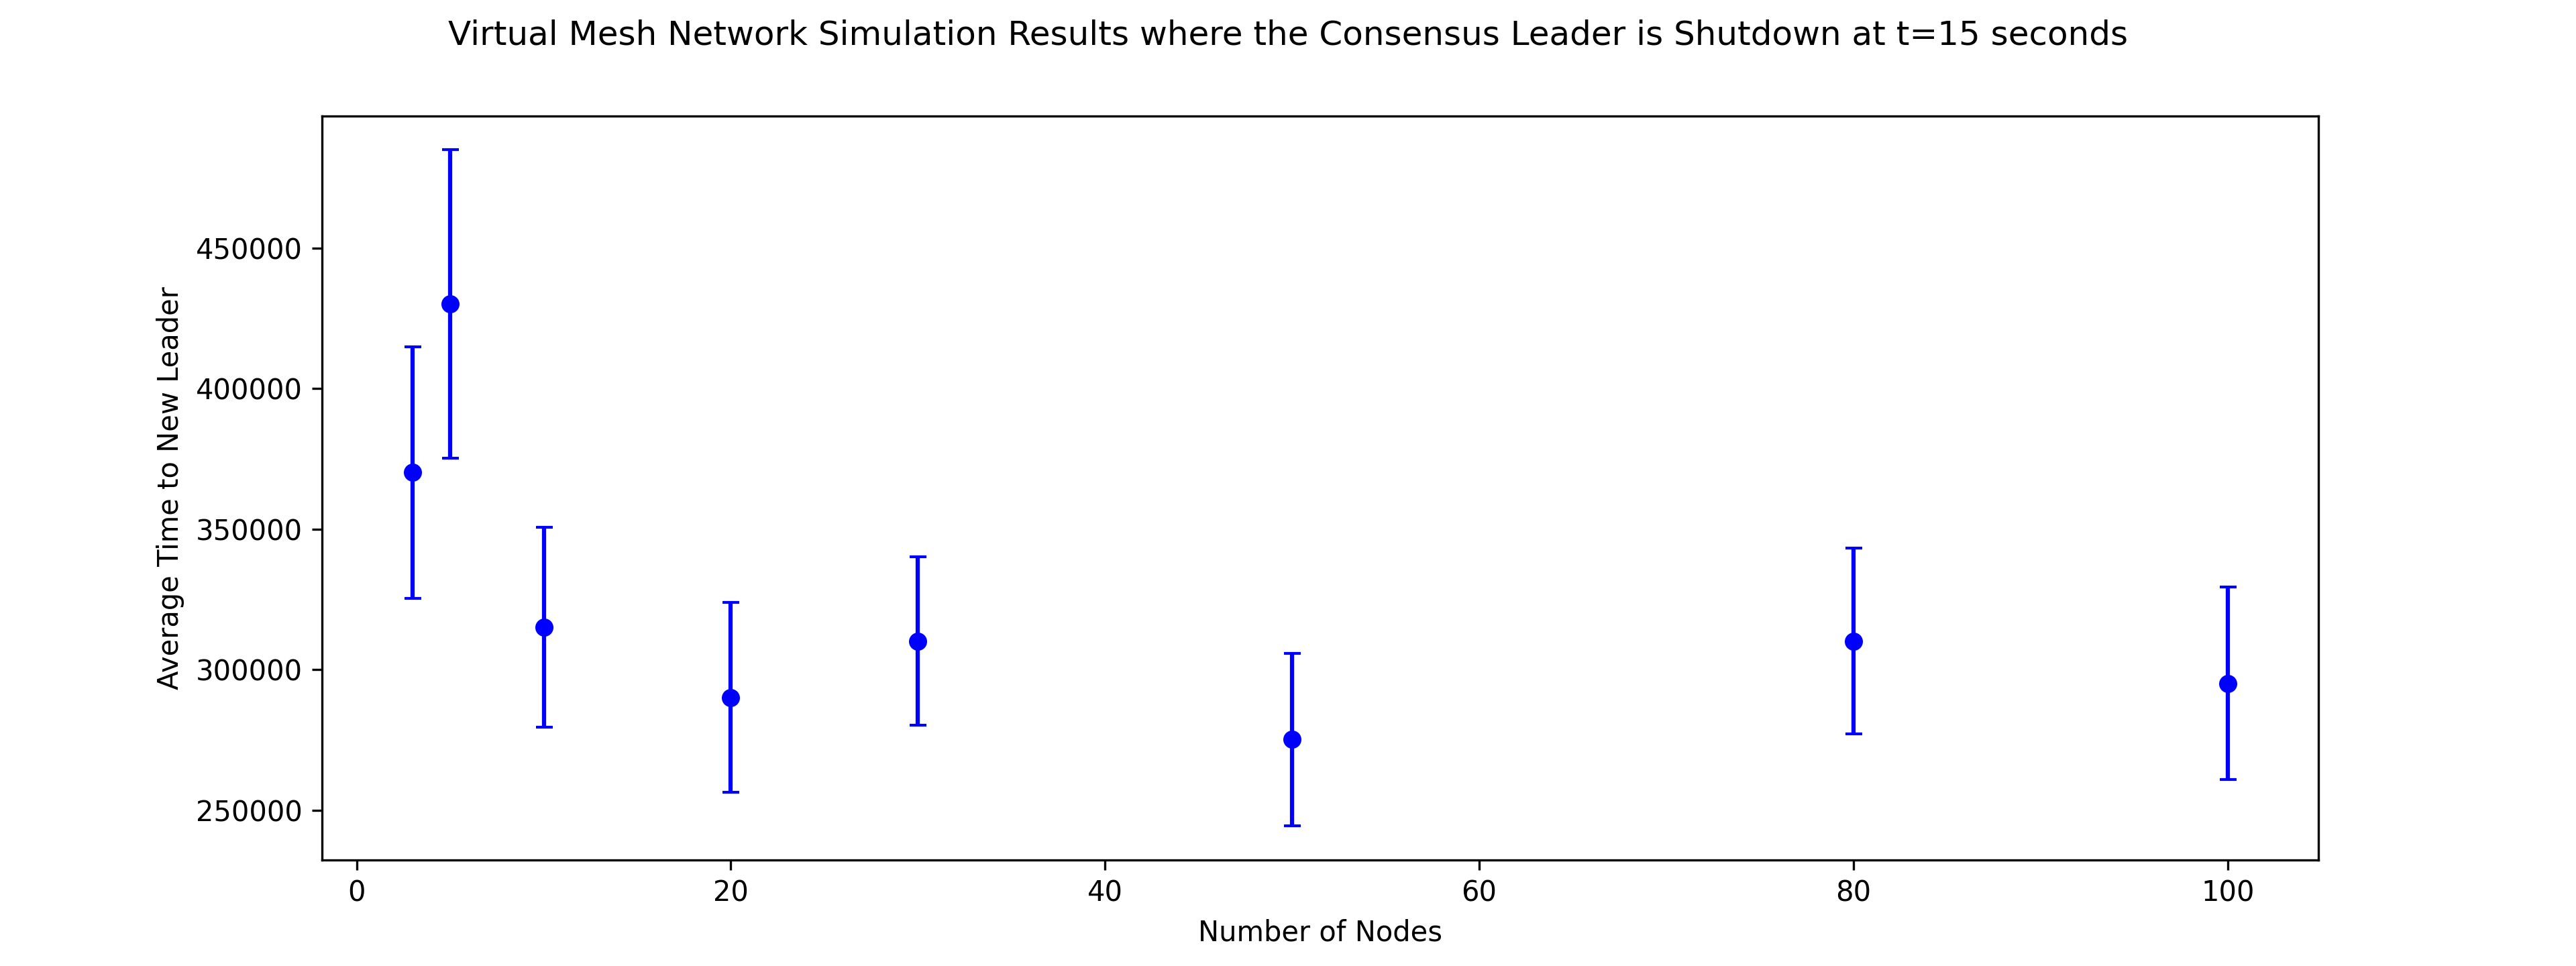
\includegraphics[width=0.9\columnwidth]{images/virtual_vary_leader_kill.png}
    \caption{Average time to elect new leader per number of nodes when the leader is shutdown}
    \label{fig:virtual_vary_leader_kill}
\end{figure}


\begin{figure}[H]
    \centering
    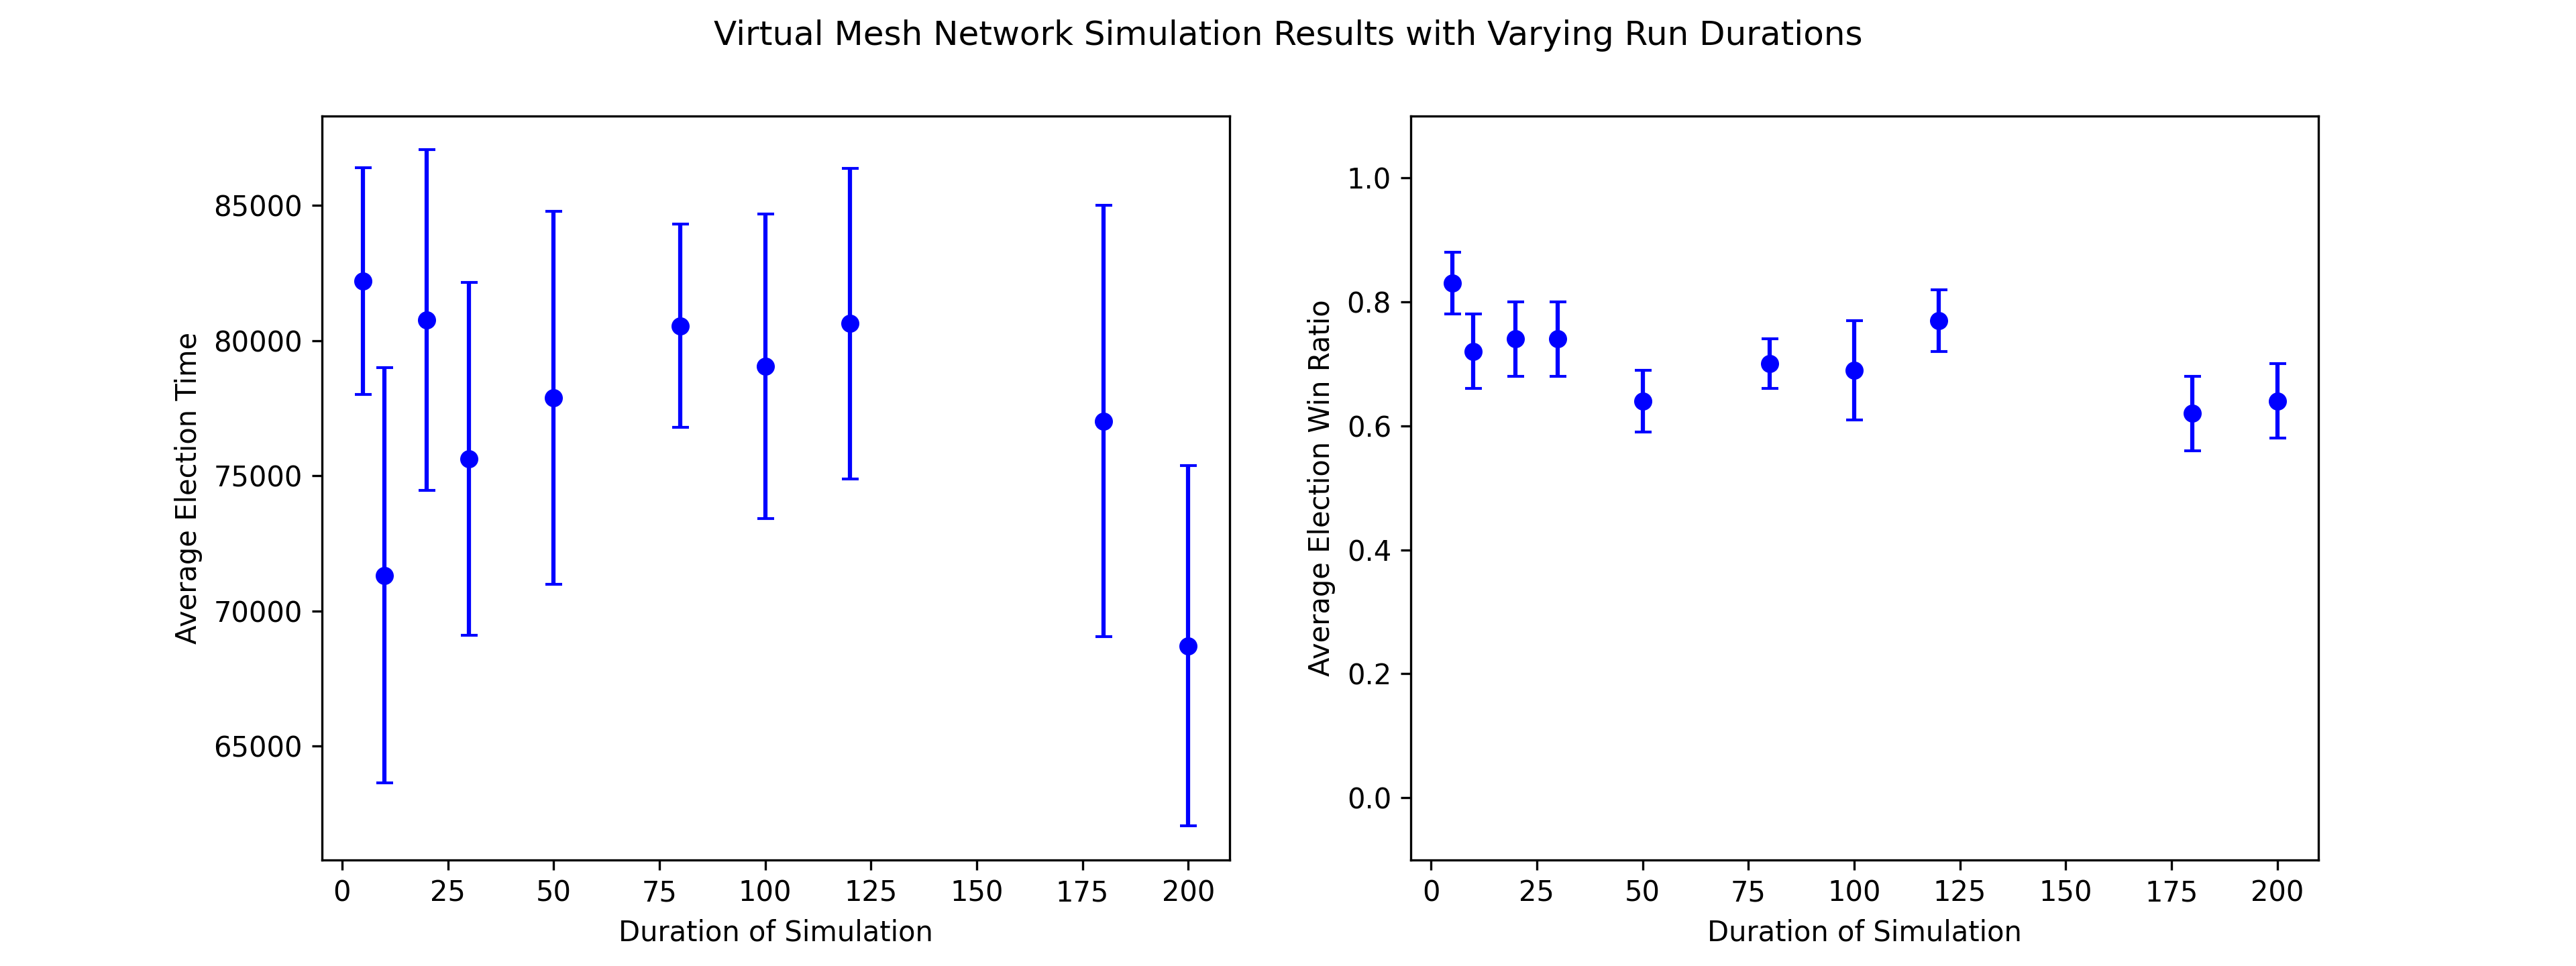
\includegraphics[width=0.9\columnwidth]{images/virtual_vary_duration.png}
    \caption{Left:Average election time per change in simulation run duration, Right: Average ratio of elections won to initiated per change in simulation run duration}
    \label{fig:virtual_vary_duration}
\end{figure}


\begin{figure}[H]
    \centering
    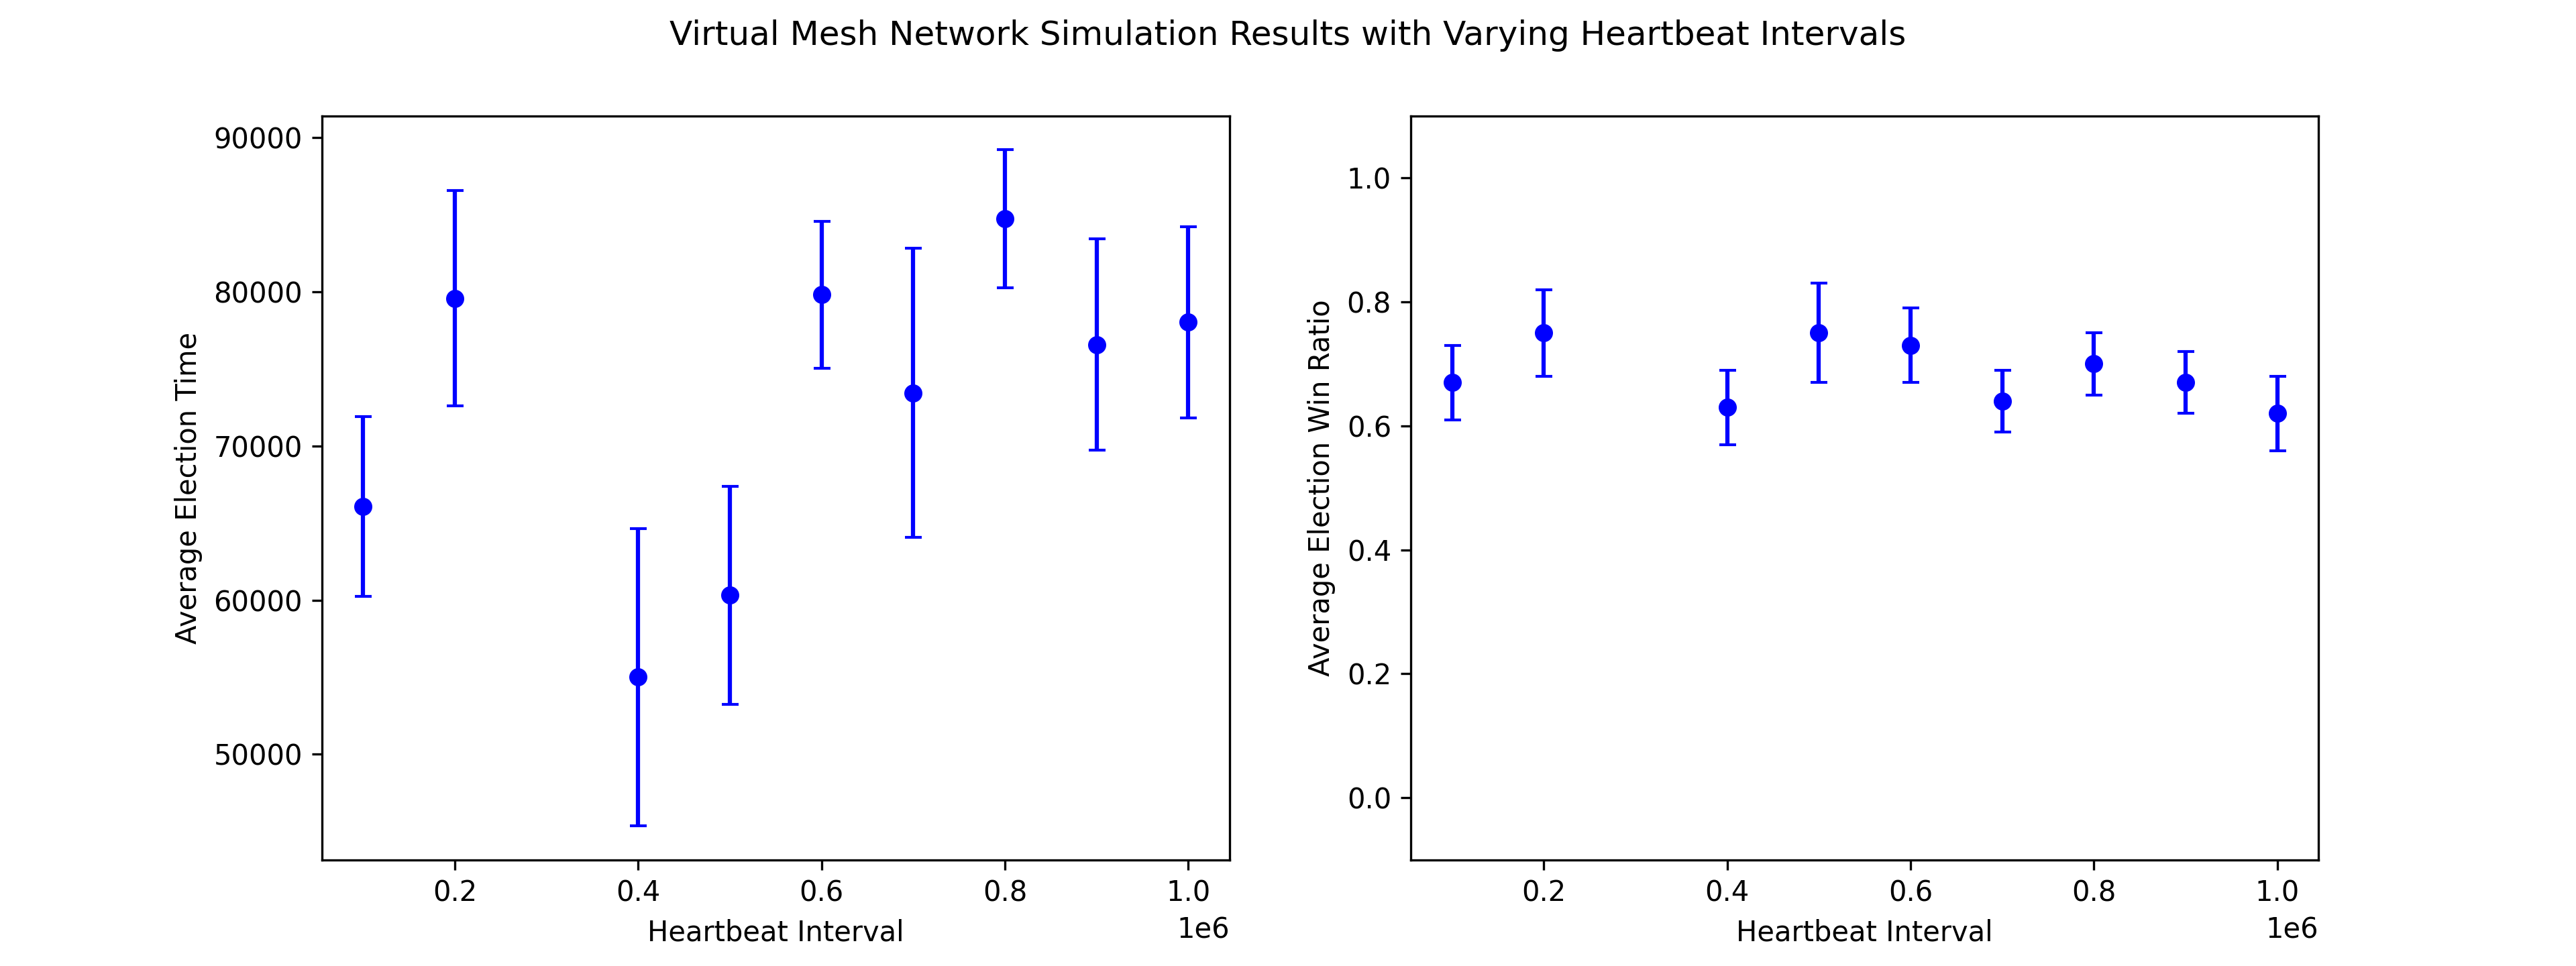
\includegraphics[width=0.9\columnwidth]{images/virtual_vary_heartbeat.png}
    \caption{Left: Average election time per change in heartbeat interval, Right: Average ratio of elections won to initiated per change in heartbeat interval}
    \label{fig:virtual_vary_heartbeat}
\end{figure}


\begin{figure}[H]
    \centering
    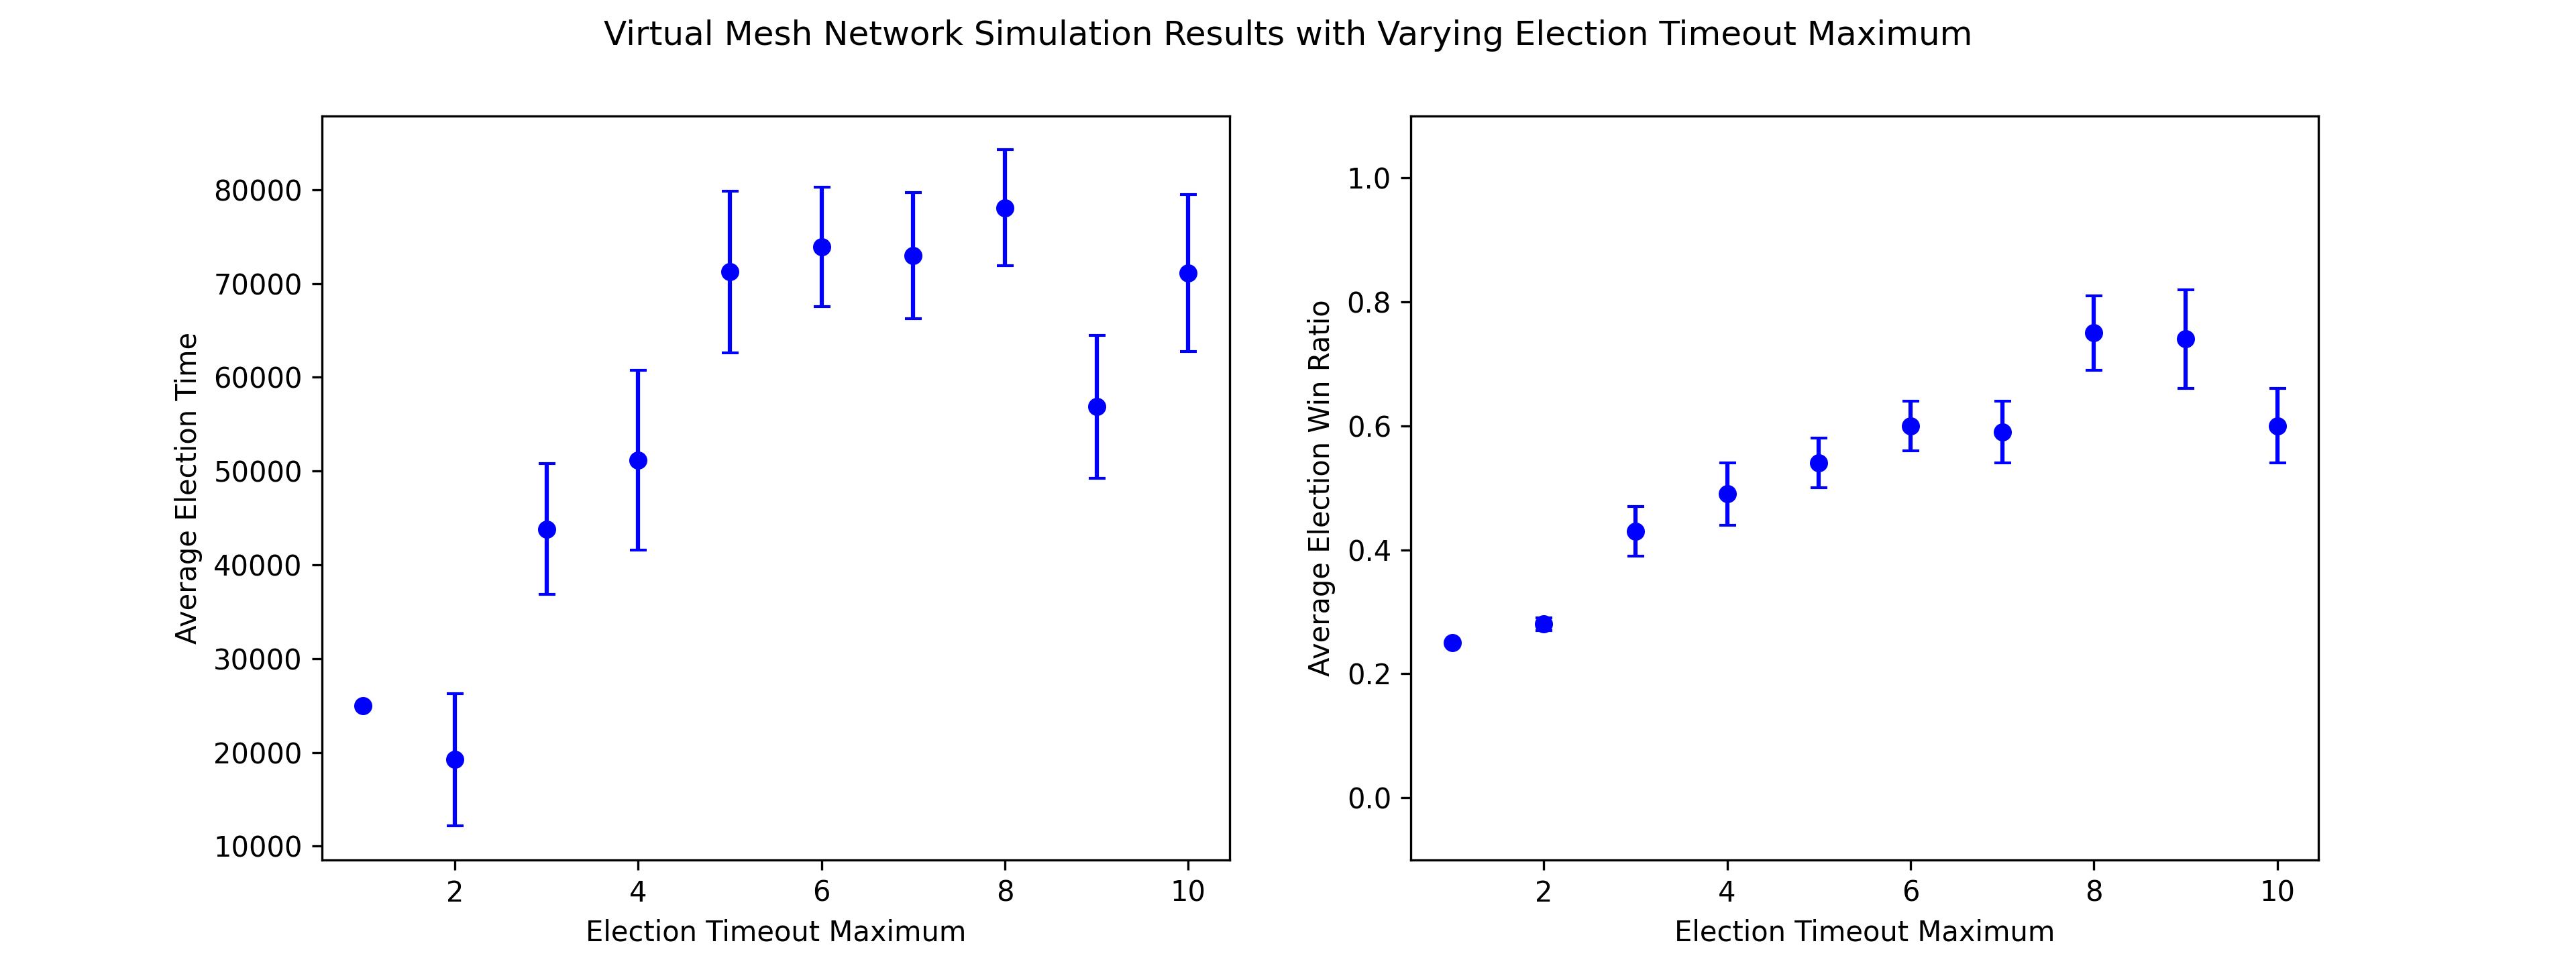
\includegraphics[width=0.9\columnwidth]{images/virtual_vary_election_timeout.png}
    \caption{Left:Average election time per change in maximum possible election timeout, Right: Average ratio of elections won to initiated per change in maximum possible election timeout}
    \label{fig:virtual_vary_election_timeout}
\end{figure}


\subsubsection{Meeting the Specifications}

\begin{table}[H]
    \centering
    \footnotesize
    \renewcommand{\arraystretch}{2.5}
    \vspace{10pt}
    \caption{Meeting the testing criteria and design constraints of the capstone project}
    \label{tab:meeting_the_specificatons}
    \begin{tabular}{|l|p{5cm}|p{5cm}|}
        \hline
        \textbf{Testing Criterion}   & \textbf{Specifications} & \textbf{Meeting the Specifications} \\ 
        \thickhline 
        Resilient to threats  & The network should recovering from the loss of a consensus leader within 1000\si{\ms} & In average it takes 300 \si{\ms} for a new leader to be elected after a failure as shown in Figure \ref{fig:virtual_vary_leader_kill}. \\ \hline
        Scalability           & The network should support at least 100 nodes in an area covering 1000\si{m^2} & The network can support more than 100 nodes.  \\ \hline
        Low power consumption & The board should consume below 100\si{mA} on average use while running the library & The board consumes 91\si{mA} on average use while running the library. \\ \hline
        Small footprint       & The compiled library should fit into an embedded 2\si{MB} flash memory. & The compiled code takes up  0.33\si{MB} of space in the flash memory. \\ \hline
    \end{tabular}
\end{table}


\subsection{Discussion}

We were able to successfully implement the Raft consensus algorithm for embedded systems atop a mesh network. The measured performance of our software library complements the results we obtained from our modeling and Coracle simulation results. Figure \ref{fig:virtual_vary_nodes} shows that there is not a drastic drop in performance as the network size increases; the decrease and eventual plateau in the election win to started ratio are expected and on par with our simulations, as shown in Figure \ref{fig:coracle_vary_nodes}. Figure \ref{fig:virtual_vary_leader_kill} shows the results of shutting down the consensus leader halfway through the simulation and measuring the time it takes to re-elect a new leader. We see that as the network size grows, the time to re-election is not significantly affected. Furthermore, in Figure \ref{fig:virtual_vary_election_timeout}, the results seem to indicate that the optimal maximum election timeout lies between 8-9 seconds.  Otherwise, the graphs show a similar trend to the Coracle simulations, where a greater average timeout maximum leads to a greater average election time and a greater average election win ratio.

Changing the run duration of the simulation and changing the heartbeat interval does not seem to have a significant effect on the system, as evidenced by the large standard error bars in Figure \ref{fig:virtual_vary_duration} and \ref{fig:virtual_vary_heartbeat}. These results are expected: running the simulation longer with no significant difference implies that the network remains stable while increasing the heartbeat interval should not have an impact on the elections. 

Therefore, overall, the obtained results suggest that our implementation meets the design requirements for creating a resilient mesh network coupled with a consensus algorithm.
% \section{Deliverables Statement}

By the end of this project, we will deliver the following: 

\begin{enumerate}
  \item An open-source software library that implements the Raft consensus algorithm for use with a mesh-network as shown in Figure \ref{fig:del_black_box}
  \item A minimal prototype board with an ESP8266 microprocessor developed to demonstrate the capabilities of the software library.
  \item A capstone report outlining our progress and the documentation of our work.
  \item A capstone presentation outlining our progress and the documentation of our work.
  \item A capstone poster outlining our progress and the documentation of our work.
\end{enumerate}

\begin{figure}[H]
    \centering
    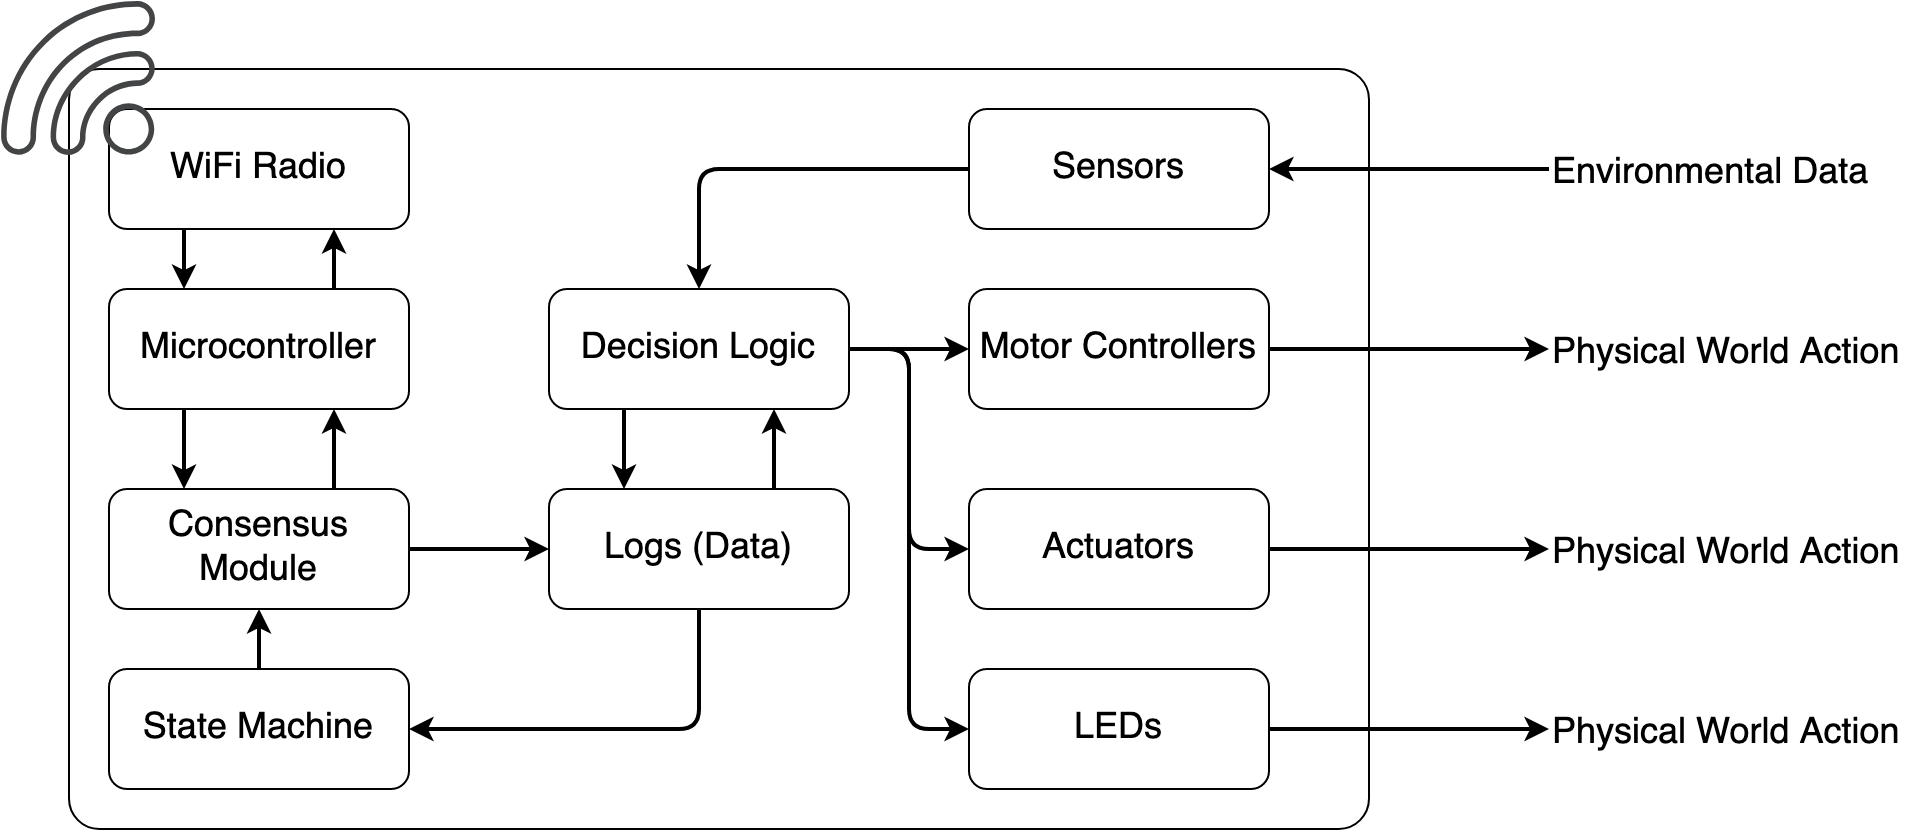
\includegraphics[width=0.65\columnwidth]{final-proposal/images/deliverable_blackbox.png}
    \caption{A black box diagram representing each node of the system}
    \label{fig:del_black_box}
\end{figure}
 % we don't need this
% \section{Criteria for Design Evaluation and Testing}
%\subsection{Evaluation Criteria}
%\subsection{Testing Criteria}
We will evaluate and test our design according to the following metrics:

\begin{itemize}
    \item \textit{Network Stability:}
    \begin{itemize}
        \item Defined as the percentage of packets delivered to the destination (PDR).
        \item The final design will be tested to see if it can achieve a PDR of greater than 85\%.
    \end{itemize}
    
    \item \textit{Network Realignment Time:}
    \begin{itemize}
        \item Defined as the time taken for all of the nodes to arrive to a consensus after the introduction of a new node. 
        \item The final design will be tested to recover and realign itself in 1000\si{ms}.
    \end{itemize}
    
    \item \textit{Data Transfer Speed \& Bandwidth:}
    \begin{itemize}
        \item Defined as the bits per second data transmission rate between nodes.
        \item The final design will be tested to see if it can achieve a data rate of 8\si{Mbps} between nodes.
    \end{itemize}
    
    \item \textit{Power Consumption:}
    \begin{itemize}
        \item Defined as the power consumption in watt measured on-board during a test session. 
        \item The final design will be tested to consume lower than 100\si{mAh} on average for 10 hours usage.
    \end{itemize}
    
    \item \textit{Scalability \& Coverage:}
    \begin{itemize}
        \item Defined as the number of nodes that can be a part of the network before deprecation of network quality within an area \si{m^2}. 
        \item The final design will be tested to operate with 500 nodes in 1000\si{m^2}.
    \end{itemize}
    
    \item \textit{Footprint}
    \begin{itemize}
        \item Defined as the storage space the library takes. 
        \item The final compiled code will be tested to fit within 2\si{MB} of flash memory.
    \end{itemize}
\end{itemize} % we don't need this

%%%%%%% PROJECT MANAGEMENT %%%%%%%
\newpage
\section{Project Management}
\subsection{Work Breakdown Structure}
The project was broken down into sub-tasks, and each subtask's length of completion was estimated in days as shown in Table \ref{tab:work_breakdown_structure}. The \emph{work breakdown structure} has been designed to keep the project on track but is flexible enough to allow for any future adjustments needed to complete the project successfully.

\textit{Table \ref{tab:work_breakdown_structure} only captures the two highest levels of work breakdown due to space constraints. Further levels of work can be found in our \href{https://github.com/A5-015/ramen/issues?q=is\%3Aissue+sort\%3Aupdated-desc}{GitHub issues webpage.} We decided to choose this method due to its dynamic nature.}

\textit{Here is the link to our GitHub issues webpage:}\\
\url{https://github.com/A5-015/ramen/issues}

\begin{table}[H]
    \scriptsize
    
    % Set row height
    \renewcommand{\arraystretch}{1.125}
    
    %%%%%%%%%%%%%%%%%%%%%%%%%%%%%%%%%%
    %%%%%%%% HELPER FUNCTIONS %%%%%%%% 
    %%%%%%%%%%%%%%%%%%%%%%%%%%%%%%%%%%
    
    % Set current date [YYYY-MM-DD]
    \newcommand{\setCurrDate}[3]{\setdatenumber{#1}{#2}{#3}}
    
    % Custom date format
    \def\datedate{\thedatemonth/\thedateday/\thedateyear}
    %\def\datedate{\thedateday-\thedatemonth-\thedateyear}
    
    % Takes number of days as an argument and prints "arg1 & DATE & DATE+arg1"
    \newcommand{\TEdate}[1]{
        \setdatebynumber{\thedatenumber}
        \multicolumn{1}{c}{#1} & 
        \datedate & 
        \addtocounter{datenumber}{#1} \setdatebynumber{\thedatenumber}
        \datedate
    }
    
    % Stuff for numbering table items
    \newcounter{TableEntryID}
    \newcounter{SubTableEntryID}
    \setcounter{SubTableEntryID}{0}
    \setcounter{TableEntryID}{0}
    \newcommand\showTE{\setcounter{SubTableEntryID}{0}\stepcounter{TableEntryID}\theTableEntryID.\theSubTableEntryID \ }
    \newcommand\showSubTE{\stepcounter{SubTableEntryID}\theTableEntryID.\theSubTableEntryID \ }
    
    % Stuff for automating table rows
    \newcommand{\tableEntry}[1]{\hline \multirow{2}{*}{\showTE #1}}
    \newcommand{\subTableEntry}[2]{& \showSubTE #1 & \TEdate{#2} \\ \cline{2-5}}
    \newcommand{\initialTableEntry}[2]{&0.1 #1 & \TEdate{#2} \\ \cline{2-5}}
    \newcommand{\finalTableEntry}[2]{\hline &\showTE #1 & \TEdate{#2} \\ \hline}
    
    \vspace{10pt}
    \caption{Work breakdown structure of the project}
    \label{tab:work_breakdown_structure}
    
    \begin{center}
        \begin{tabular}{|l|p{30em}|p{3.5em}|r|r|}
            % Table HEAD
            \hline
            \multicolumn{2}{|l|}{\multirow{3}{9cm}{\textbf{ramen: Design and Development of a Raft Consensus Algorithm Coupled With a IEEE 802.11 Based Mesh Network for Embedded Systems}}} & \multicolumn{3}{c|}{Dates and Duration} \\ \cline{3-5}
            \multicolumn{2}{|l|}{ } & Duration (Days) & \multicolumn{2}{c|}{Planned Dates} \\ \cline{3-5}
            \multicolumn{2}{|l|}{ } & & \multicolumn{1}{c}{Start} & \multicolumn{1}{|c|}{End} \\ \hline
            
            %%%%%%%%%%%%%%%%%%%%%%%%%%%%%%%%%%%%%%%%%%%%%%%
            %%%%%%%% ACTUAL TABLE DATA STARTS HERE %%%%%%%% 
            %%%%%%%%%%%%%%%%%%%%%%%%%%%%%%%%%%%%%%%%%%%%%%%
            
            \setCurrDate{2020}{09}{06}
            \initialTableEntry{Begin Project}{1}
            
        	\tableEntry{Background Research}
        	    \subTableEntry{Research on existing problems in IoT devices}{3}
            	\subTableEntry{Research on existing problems in embedded devices}{3}
            	\subTableEntry{Research on currently existing solutions}{3}
            	\subTableEntry{Identifying technical \& non-technical constraints}{4}
            	\subTableEntry{Revise problem statement}{1}
        	
        	\tableEntry{Generate Concepts}
        	    \subTableEntry{Functionality decompose of the project}{1}
            	\subTableEntry{Research on literature for similar solutions}{5}
             	\subTableEntry{Experimenting with existing consensus and mesh networking protocols protocols}{3}
             	\subTableEntry{Consensus protocol, network topology, and  microprocessors selection}{2}
            	
        	\tableEntry{Begin Detailed Design}
        	    \subTableEntry{Perform detailed analysis of the concepts}{2}
        	    \subTableEntry{Perform detailed analysis of the available components}{5}
        	    \subTableEntry{Select components}{2}
            	\subTableEntry{Perform simulations with consensus algorithms}{5}
            	\subTableEntry{Perform simulations with WiFi chips}{5}
            	\subTableEntry{Create workflow diagrams for the code}{2}
        	
        	\tableEntry{Build Prototype}
        	    \subTableEntry{Create a GitHub repository}{1}
        	    \subTableEntry{Code a mesh network for ESP8266 chip}{20}
        	    \subTableEntry{Adapt the Raft consensus algorithm for mesh networks}{25}
        	    \subTableEntry{Code an adapter for our Raft implementation for ESP8266 chip specifically}{25}
        	    \subTableEntry{Ensure the functionality of connection between the Raft consensus algorithm implementation and the mesh networking adapter}{5}
        	    \subTableEntry{Write tests for the code}{5}
            	\subTableEntry{CAD drawings for the enclosure}{4}
            	\subTableEntry{Design the PCB}{10}
            	\subTableEntry{Order the PCB for fabrication}{2}
            	\subTableEntry{Purchase the PCB components}{5}
            	\subTableEntry{Assemble the PCB}{3}
            	\subTableEntry{3D printing the enclosure}{2}
            	\subTableEntry{Assembling the prototype}{3}
            	\subTableEntry{Upload the code to the prototype}{2}
            	\subTableEntry{Check the functionality of the prototype and the code}{5}
        	
        	\tableEntry{Test Prototype}
            	\subTableEntry{Develop testing protocol}{7}
            	\subTableEntry{Perform tests}{7}
        	
        	\tableEntry{Documentation and Reporting}
        	    \subTableEntry{Generating documentation from the code}{2}
            	\setCurrDate{2020}{10}{01}\subTableEntry{Preparation of the Intermediary Report I}{10}
            	\setCurrDate{2020}{11}{20}\subTableEntry{Preparation of the Final Proposal}{10}
            	\subTableEntry{Preparation of the Proposal Presentation}{8}
            	\setCurrDate{2021}{2}{18}\subTableEntry{Preparation of the Intermediary Report II}{10}
            	\setCurrDate{2021}{4}{20}\subTableEntry{Preparation of the Final Poster}{8}
            	\subTableEntry{Preparation of the Final Report}{3}
        	
        	\finalTableEntry{End Project}{1}
        	
        \end{tabular}
    \end{center}
\end{table}


\newpage
\subsection{Design Structure Matrix}
To complement the \emph{work breakdown structure}, a \emph{design structure matrix}, shown in Table \ref{tab:design_structure_matrix}, was created. The \emph{design structure matrix} is meant to organize our tasks and streamline our workflow.


\begin{table}[H]
    \scriptsize
    \centering
    \renewcommand{\arraystretch}{1.3}
    \vspace{10pt}
    \caption{Design structure matrix of the project}
    \label{tab:design_structure_matrix}
    \begin{tabular}{r|c|c|c|c|c|c|c|c|c|c|c|c|c|c|c|}
        \cline{2-16}
                                        &   & A & B & C & D & E & F & G & H & I & J & K & L & M & N \\ \cline{2-16}
         Begin Project                  & A & A &   &   &   &   &   &   &   &   &   &   &   &   &   \\ \cline{2-16}
         Background Research            & B & X & B &   &   &   &   &   &   &   &   &   &   &   &   \\ \cline{2-16}
         Consensus Algorithm Selection  & C &   & X & C &   &   &   &   &   &   &   &   &   &   &   \\ \cline{2-16}
         Network Topology Selection     & D &   & X &   & D &   &   &   &   &   &   &   &   &   &   \\ \cline{2-16}
         Concept Generation             & E &   &   & X & X & E &   &   &   &   &   &   &   &   &   \\ \cline{2-16}
         Detailed Design                & F &   &   & X & X & X & F &   &   &   &   &   &   &   &   \\ \cline{2-16}
         Simulation                     & G &   &   &   &   &   & X & G &   &   &   &   &   &   &   \\ \cline{2-16}
         Finalize Design                & H &   &   &   &   &   & X & X & H &   &   &   &   &   &   \\ \cline{2-16}
         Coding the software            & I &   &   & X & X & X &   & X & X & I &   &   &   &   &   \\ \cline{2-16}
         CAD Drawings                   & J &   &   &   &   &   &   & X & X &   & J &   &   &   &   \\ \cline{2-16}
         Purchase Components            & K &   &   &   &   &   &   &   & X &   & X & K &   &   &   \\ \cline{2-16}
         Manufacture Components         & L &   &   &   &   &   &   &   &   &   & X & X & L &   &   \\ \cline{2-16}
         Assembly and Testing           & M &   &   &   &   &   &   &   & X & X &   &   & X & M &   \\ \cline{2-16}
         Finish Project                 & N &   &   &   &   &   &   &   &   &   &   &   &   & X & N \\
        \cline{2-16}
    \end{tabular}
\end{table}


\subsection{Critical Path}
The \emph{critical path method} was used to identify the bottlenecks in the project. The duration for each project component was calculated in days and placed into the \emph{critical path} graph shown in Figure \ref{fig:critical_path}. After our analysis, we have determined that the critical path for our project is to implement the base software library, explore the implementation of a mesh network, adapt our library to interface with the mesh network and finally test our implementation.

\begin{figure}[H]
    \centering
    
    \resizebox{0.80\pdfpagewidth}{!}{
        \begin{tikzpicture}
        
            %%%%%%%%%%%%%%%%%%%%%%%%%%%%%%%%%%
            %%%%%%%% HELPER FUNCTIONS %%%%%%%% 
            %%%%%%%%%%%%%%%%%%%%%%%%%%%%%%%%%%
            
            % Custom color
            \definecolor{airforceblue}{rgb}{0.36, 0.54, 0.66}
            
            % Function for generating nodes in the graph
            \newcommand{\pathNode}[5][black]{
                \scriptsize
                \node(#2)[shape=rectangle][#3] {
                    \begin{tcolorbox}[
                        rounded corners,
                        colback=airforceblue!35,
                        colframe=#1!80,
                        arc=1.5mm,
                        box align=center,
                        halign=center,
                        valign=center,
                        text width=2cm,
                        left=0.5mm,
                        right=0.5mm,
                        top=0.5mm,
                        bottom=0.5mm,
                        title = {\centering\makebox[\linewidth][c]{\color{white}#5 Days}}
                    ]
                    \color{black}#4
                    \end{tcolorbox} \\
                };
            }
            
            % Function for generating a terminal node (like start % end) in the graph
            \newcommand{\terminalNode}[4][black]{
                \scriptsize
                \node(#2)[circle, draw=#1!80, fill=airforceblue!35, very thick, minimum size=7mm][#3]{#4};
            }
            
            % Function for drawing the arrows
            \newcommand{\pathArrow}[2]{
                \draw[->, very thick] (#1) -- (#2);
            }
        
            %%%%%%%%%%%%%%%%%%%%%%%%%%%%%%%%%%%%%%%%%%%%%%%
            %%%%%%%% ACTUAL GRAPH DATA STARTS HERE %%%%%%%% 
            %%%%%%%%%%%%%%%%%%%%%%%%%%%%%%%%%%%%%%%%%%%%%%%
            
            % Nodes
            \terminalNode[red]{start}{}{Capstone Project}
            
            \pathNode[red]{software_1}{above right = of start, yshift=1cm, xshift=1cm}{Implement the Raft consensus algorithm for embedded systems}{30}
            \pathNode[red]{software_4}{above right = of software_1, yshift=-1.25cm}{Creating an interface to work with painlessMesh}{20}
            \pathNode[red]{software_5}{right = of software_4}{Developing a virtual simulation environment to test our Raft implementation}{15}
            \pathNode{software_2}{below right = of software_1, yshift=1.25cm, xshift=2cm}{Running Raft consensus algorithm simulations in Coracle software for various network conditions}{20}
            \pathNode[red]{software_3}{below right = of software_5, yshift=1cm}{Testing the code in a simulation for optimization}{15}
            
            
            \pathNode{hardware_1}{below right = of start, xshift=1cm}{Component selection}{15}
            \pathNode{hardware_4}{below right = of hardware_1, yshift=1.25cm}{Prototype enclosure design}{10}
            \pathNode{hardware_2}{above right = of hardware_1, yshift=-1.25cm}{Schematic design}{10}
            \pathNode{hardware_3}{right = of hardware_2}{PCB Design}{10}
            \pathNode{hardware_5}{right = of hardware_4}{Manufacturing Components}{15}
            
            
            \pathNode[red]{software_6}{right = of hardware_3, xshift=2.25cm}{Testing on the hardware}{10}
            
            % Arrows
            \pathArrow{start.east}{software_1.west}
            \pathArrow{start.east}{hardware_1.west}
            
            \pathArrow{software_1.east}{software_2.west}
            \pathArrow{software_1.east}{software_2.west}
            \pathArrow{software_1.east}{software_4.west}
            \pathArrow{software_4.east}{software_5.west}
            \pathArrow{software_2.east}{software_3.west}
            \pathArrow{software_5.east}{software_3.west}
            \pathArrow{software_3.south}{software_6.west}
            
            %\pathArrow{software_5.south}{software_2.north}
            
            \pathArrow{hardware_1.east}{hardware_4.west}
            \pathArrow{hardware_1.east}{hardware_2.west}
            \pathArrow{hardware_2.east}{hardware_3.west}
            \pathArrow{hardware_3.south}{hardware_5.north}
            \pathArrow{hardware_4.east}{hardware_5.west}
            \pathArrow{hardware_4.east}{hardware_3.west}
            \pathArrow{hardware_5.east}{software_6.west}
            
            \pathArrow{hardware_2.north}{software_2.west}
    
        \end{tikzpicture}
    }
    \caption{Critical path of the project tasks}
    \label{fig:critical_path}
\end{figure}





\newpage
\subsection{Gantt Chart}
The \emph{Gantt Chart} shown in Figure \ref{fig:gantt} was used to visualize the tasks and their duration. The \emph{Gantt Chart} is meant to track our progress on the sub-tasks and overall progress on the project.

\vspace{5mm}

\ganttset{calendar week text = \small {\startday}}

\hvFloat[rotAngle=0]{figure}{
    \resizebox{0.8\pdfpagewidth}{!}{
        \begin{ganttchart}[
            newline shortcut=true,
            bar label node/.append style={align=right},
            time slot format = isodate, 
            vgrid = {*{6}{dotted}, *{1}{dashed}},
            hgrid,x unit=1mm,
            hgrid style/.style={draw=black!5, line width=.75pt},
            time slot format=little-endian,
            linespacing=0.5]
            {01-09-2020}{15-06-2021}
            \gantttitlecalendar{year, month=shortname, week=4}\\
            %%%%%%%%%%%%
            \ganttgroup{Background Research}{07-09-2020}{21-09-2020} \\
                \ganttbar{Research on existing problems}{7-9-2020}{13-9-2020} \\
                \ganttbar{Research on currently existing solutions}{13-9-2020}{16-9-2020} \\
                \ganttbar{Identifying technical \& non-technical constraints}{16-9-2020}{21-9-2020} \\
            %%%%%%%%%%%%
            \ganttgroup{Generate Concepts}{21-09-2020}{02-10-2020} \\
                \ganttbar{Functionality decompose of the project}{21-9-2020}{22-9-2020} \\
                \ganttbar{Research on literature for similar solutions}{22-9-2020}{27-9-2020} \\
                \ganttbar{Experimenting with existing consensus \ganttalignnewline and mesh networking protocols protocols}{27-9-2020}{30-9-2020} \\
                \ganttbar{Consensus protocol, network topology, \ganttalignnewline and  microprocessors selection}{30-9-2020}{02-10-2020} \\
            %%%%%%%%%%%%
            \ganttgroup{Begin Detailed Design}{02-10-2020}{23-10-2020} \\
                \ganttbar{Perform detailed analysis of the concepts}{02-10-2020}{09-10-2020} \\
                \ganttbar{Select components}{09-10-2020}{11-10-2020} \\
                \ganttbar{Build development environment for Coracle simulations}{11-10-2020}{23-10-2020} \\
            %%%%%%%%%%%%
            \ganttgroup{Build Prototype}{23-10-2020}{17-02-2021} \\
                \ganttbar{Implement Raft for embedded systems}{23-10-2020}{13-11-2020} \\
                \ganttbar{Create interface for painlessMesh}{13-11-2020}{8-12-2020} \\
                \ganttbar{Develop a virtual simulation environment for our implementation}{8-12-2020}{12-1-2021} \\
                \ganttbar{PCB design and CAD drawings}{12-1-2021}{28-1-2021} \\
                \ganttbar{Purchase the PCB components}{28-1-2021}{2-2-2021} \\
                \ganttbar{Assembling the prototype}{2-2-2021}{17-2-2021} \\
            %%%%%%%%%%%%
            \ganttgroup{Test Prototype}{17-02-2021}{03-03-2021} \\
                \ganttbar{Develop testing protocol in virtual environment}{17-2-2021}{24-2-2021} \\
                \ganttbar{Perform tests on custom PCBs}{24-2-2021}{24-3-2021} \\
            %%%%%%%%%%%%
            \ganttgroup{Documentation and Reporting}{24-03-2021}{08-05-2021} \\
                \ganttbar{Generating documentation from the code}{24-3-2021}{05-4-2021} \\
                \ganttbar{Preparing Reports, Presentations, and Posters}{05-4-2021}{08-05-2021} \\
            %%%%%%%%%%%%
        \end{ganttchart}
    }
}[The Gantt Chart of the project timeline]{The Gantt Chart of the project timeline}{fig:gantt}

%%%%%%% BIBLIOGRAPHY %%%%%%%
\newpage
\printbibliography[heading=bibintoc,title={References}]

%%%%%%% APPENDIX %%%%%%%
\newpage
\appendices

\newpage
\section{Pugh Charts}
\label{sec:pugh-chart-appendix}

\subsection{Networking Library}

\begin{table}[!h]
    \scriptsize
    
    % Set row height
    \renewcommand{\arraystretch}{1.3}
    \vspace{10pt}
    
    \caption{Pugh chart for networking library with easyMesh as base}
    \label{tab:pugh_raft}

    \begin{center}
        \begin{tabular}{@{}*{6}{|p{0.14\textwidth}|@{}}}
        \hline
        \multicolumn{1}{|c|}{Networking Library} & Documentation & Compatibility & Routing Method & Framework Restriction & Sum \\
        \thickhline
        easyMesh         & Base & Base & Base & Base &   \\ \hline
        painlessMesh     & 1 & 0 & 0 & 0 & 1 \\ \hline
        ESP-MESH         & 1 & -1 & 0 & 0 & 0\\ \hline
        ESP8266 Wifi Mesh & 0 & 0 & -1 & -1 & -2  \\ \hline
        \end{tabular}
    \end{center}
\end{table}
\FloatBarrier

\begin{table}[!h]
    \scriptsize
    
    % Set row height
    \renewcommand{\arraystretch}{1.3}
    \vspace{10pt}
    
    \caption{Pugh chart for networking library with painlessMesh as base}
    \label{tab:pugh_raft}

    \begin{center}
        \begin{tabular}{@{}*{6}{|p{0.14\textwidth}|@{}}}
        \hline
        \multicolumn{1}{|c|}{Networking Library} & Documentation & Compatibility & Routing Method & Framework Restriction & Sum \\
        \thickhline
        easyMesh         & -1 & 0 & 0 & 0 & -1 \\ \hline
        painlessMesh     & Base & Base & Base & Base &   \\ \hline
        ESP-MESH         & 1 & -1 & 0 & 0 & -1 \\ \hline
        ESP8266 Wifi Mesh & -1 & 0 & -1 & -1 & -3 \\ \hline
        \end{tabular}
    \end{center}
\end{table}
\FloatBarrier

\begin{table}[!h]
    \scriptsize
    
    % Set row height
    \renewcommand{\arraystretch}{1.3}
    \vspace{10pt}
    
    \caption{Pugh chart for networking library with ESP-MESH as base}
    \label{tab:pugh_raft}

    \begin{center}
        \begin{tabular}{@{}*{6}{|p{0.14\textwidth}|@{}}}
        \hline
        \multicolumn{1}{|c|}{Networking Library} & Documentation & Compatibility & Routing Method & Framework Restriction & Sum \\
        \thickhline
        easyMesh         & -1 & 1 & 0 & 0 & 0 \\ \hline
        painlessMesh     & -1 & 1 & 0 & 0 & 0 \\ \hline
        ESP-MESH         & Base & Base & Base & Base &   \\ \hline
        ESP8266 Wifi Mesh & -1 & 1 & -1 & -1 & -4 \\ \hline
        \end{tabular}
    \end{center}
\end{table}
\FloatBarrier

\begin{table}[!h]
    \scriptsize
    
    % Set row height
    \renewcommand{\arraystretch}{1.3}
    \vspace{10pt}
    
    \caption{Pugh chart for networking library with ESP8266 Wifi Mesh as base}
    \label{tab:pugh_raft}

    \begin{center}
        \begin{tabular}{@{}*{6}{|p{0.14\textwidth}|@{}}}
        \hline
        \multicolumn{1}{|c|}{Networking Library} & Documentation & Compatibility & Routing Method& Framework Restriction & Sum \\
        \thickhline
        easyMesh          & 1 & 0 & 1 & 1 & 3 \\ \hline
        painlessMesh      & 0 & 0 & 1 & 1 & 2 \\ \hline
        ESP-MESH          & 1 & -1 & 1 & 1 & 2 \\ \hline
        ESP8266 Wifi Mesh & Base & Base & Base & Base &   \\ \hline
        \end{tabular}
    \end{center}
\end{table}
\FloatBarrier

% We see that painlessMesh is the best mesh networking library to work with given its superior documentation and compatibility with our selected hardware. 

\newpage

\subsection{Networking Topology}

\begin{table}[!h]
    \scriptsize
    
    % Set row height
    \renewcommand{\arraystretch}{1.3}
    \vspace{10pt}
    
    \caption{Pugh chart for networking topology with hub-spoke topology as base}
    \label{tab:pugh_raft}

    \begin{center}
        \begin{tabular}{@{}*{6}{|p{0.14\textwidth}|@{}}}
        \hline
        \multicolumn{1}{|c|}{Networking Topology} & Simplicity & Failure Risk & Collision & Scalability & Sum \\
        \thickhline
        Hub-Spoke   & Base & Base & Base & Base &   \\ \hline
        Mesh        & -1 & 1 & 0 & 1 & 2\\ \hline
        Ring        & 0 & -1 & 0 & 0 & -1\\ \hline
        Bus         & 0 & 1 & -1 & -1 & -1\\ \hline
        \end{tabular}
    \end{center}
\end{table}
\FloatBarrier

\begin{table}[!h]
    \scriptsize
    
    % Set row height
    \renewcommand{\arraystretch}{1.3}
    \vspace{10pt}
    
    \caption{Pugh chart for networking topology with mesh topology as base}
    \label{tab:pugh_raft}

    \begin{center}
        \begin{tabular}{@{}*{6}{|p{0.14\textwidth}|@{}}}
        \hline
        \multicolumn{1}{|c|}{Networking Topology} & Simplicity & Failure Risk & Collision & Scalability & Sum \\
        \thickhline
        Hub-Spoke   & 1 & -1 & 0 & -1 & -1\\ \hline
        Mesh        & Base & Base & Base & Base &   \\ \hline
        Ring        & 1 & -1 & 0 & 0 & 0\\ \hline
        Bus         & 1 & 0 & -1 & -1 & -1\\ \hline
        \end{tabular}
    \end{center}
\end{table}
\FloatBarrier

\begin{table}[!h]
    \scriptsize
    
    % Set row height
    \renewcommand{\arraystretch}{1.3}
    \vspace{10pt}
    
    \caption{Pugh chart for networking topology with ring topology as base}
    \label{tab:pugh_raft}

    \begin{center}
        \begin{tabular}{@{}*{6}{|p{0.14\textwidth}|@{}}}
        \hline
        \multicolumn{1}{|c|}{Networking Topology} & Simplicity & Failure Risk & Collision & Scalability & Sum \\
        \thickhline
        Hub-Spoke   & 0 & -1 & 0 & -1 & -2\\ \hline
        Mesh        & -1 & 1 & 0 & 1 & 1\\ \hline
        Ring        & Base & Base & Base & Base &   \\ \hline
        Bus         & 0 & 1 & -1 & -1 & -1\\ \hline
        \end{tabular}
    \end{center}
\end{table}
\FloatBarrier

\begin{table}[!h]
    \scriptsize
    
    % Set row height
    \renewcommand{\arraystretch}{1.3}
    \vspace{10pt}
    
    \caption{Pugh chart for networking topology with bus topology as base}
    \label{tab:pugh_raft}

    \begin{center}
        \begin{tabular}{@{}*{6}{|p{0.14\textwidth}|@{}}}
        \hline
        \multicolumn{1}{|c|}{Networking Topology} & Simplicity & Failure Risk & Collision & Scalability & Sum \\
        \thickhline
        Hub-Spoke   & 0 & -1 & 1 & 0 & 0\\ \hline
        Mesh        & -1 & 1 & 1 & 1 & 2\\ \hline
        Ring        & 0 & -1 & 1 & 1 & 1\\ \hline
        Bus        & Base & Base & Base & Base &   \\ \hline
        \end{tabular}
    \end{center}
\end{table}
\FloatBarrier

% For the applications we consider, a mesh topology is the most appropriate topology.

\newpage

\subsection{Networking Protocol}

\begin{table}[!h]
    \scriptsize
    
    % Set row height
    \renewcommand{\arraystretch}{1.3}
    \vspace{10pt}
    
    \caption{Pugh chart for networking protocol with 802.11 as base}
    \label{tab:pugh_raft}

    \begin{center}
        \begin{tabular}{@{}*{6}{|p{0.14\textwidth}|@{}}}
        \hline
        \multicolumn{1}{|c|}{Networking Topology} & Popularity & Data Rate & Power Consumption & Scalability & Sum \\
        \thickhline
        IEEE 802.11   & Base & Base & Base & Base &   \\ \hline
        IEEE 802.15.4 (Zigbee)      & -1 & -1 & 1 & 0 & -1\\ \hline
        IEEE 802.15.3 (UWB)         & -1 & 1 & 0 & -1 & -1\\ \hline
        IEEE 802.15.1 (BT)          & -1 & -1 & 1 & -1 & -2\\ \hline
        \end{tabular}
    \end{center}
\end{table}
\FloatBarrier

\begin{table}[!h]
    \scriptsize
    
    % Set row height
    \renewcommand{\arraystretch}{1.3}
    \vspace{10pt}
    
    \caption{Pugh chart for networking protocol with 802.15.4 (Zigbee) as base}
    \label{tab:pugh_raft}

    \begin{center}
        \begin{tabular}{@{}*{6}{|p{0.14\textwidth}|@{}}}
        \hline
        \multicolumn{1}{|c|}{Networking Topology} & Popularity & Data Rate & Power Consumption & Scalability & Sum \\
        \thickhline
        IEEE 802.11                 & 1 & 1 & -1 & 0 & 1\\ \hline
        IEEE 802.15.4               & Base & Base & Base & Base &   \\ \hline
        IEEE 802.15.3 (UWB)         & 0 & 1 & -1 & -1 & -1\\ \hline
        IEEE 802.15.1 (BT)          & 1 & 1 & 0 & -1 & 1\\ \hline
        \end{tabular}
    \end{center}
\end{table}
\FloatBarrier

\begin{table}[!h]
    \scriptsize
    
    % Set row height
    \renewcommand{\arraystretch}{1.3}
    \vspace{10pt}
    
    \caption{Pugh chart for networking protocol with 802.15.3 (UWB) as base}
    \label{tab:pugh_raft}

    \begin{center}
        \begin{tabular}{@{}*{6}{|p{0.14\textwidth}|@{}}}
        \hline
        \multicolumn{1}{|c|}{Networking Topology} & Popularity & Data Rate & Power Consumption & Scalability & Sum \\
        \thickhline
        IEEE 802.11                 & 1 & -1 & 0 & 1 & 1\\ \hline
        IEEE 802.15.4               & 1 & -1 & 1 & 1 & 2\\ \hline
        IEEE 802.15.3 (UWB)         & Base & Base & Base & Base &   \\ \hline
        IEEE 802.15.1 (BT)          & 1 & -1 & 1 & 0 & 1\\ \hline
        \end{tabular}
    \end{center}
\end{table}
\FloatBarrier

\begin{table}[!h]
    \scriptsize
    
    % Set row height
    \renewcommand{\arraystretch}{1.3}
    \vspace{10pt}
    
    \caption{Pugh chart for networking protocol with 802.15.1 (BT) as base}
    \label{tab:pugh_raft}

    \begin{center}
        \begin{tabular}{@{}*{6}{|p{0.14\textwidth}|@{}}}
        \hline
        \multicolumn{1}{|c|}{Networking Topology} & Popularity & Data Rate & Power Consumption & Scalability & Sum \\
        \thickhline
        IEEE 802.11                 & 1 & 1 & -1 & 1 & 2\\ \hline
        IEEE 802.15.4               & 0 & 0 & 0 & 1 & 1\\ \hline
        IEEE 802.15.3 (UWB)         & 0 & 1 & -1 & 0 & 0\\ \hline
        IEEE 802.15.1 (BT)          & Base & Base & Base & Base &   \\ \hline
        \end{tabular}
    \end{center}
\end{table}
\FloatBarrier


\newpage
\section{Code Repository}
\label{sec:appendix-for-code}

\begin{itemize}
    \item The code for the project can be found at: \href{https://github.com/A5-015/ramen}{github.com/A5-015/ramen} 
    \item The code for model generation and simulation can be founder under the "simulation" directory in the GitHub repository.
\end{itemize}



\newpage
\section{Coracle Simulation Results}
\label{sec:appendix-for-coracle-results}

\begin{figure}[H]
    \centering
    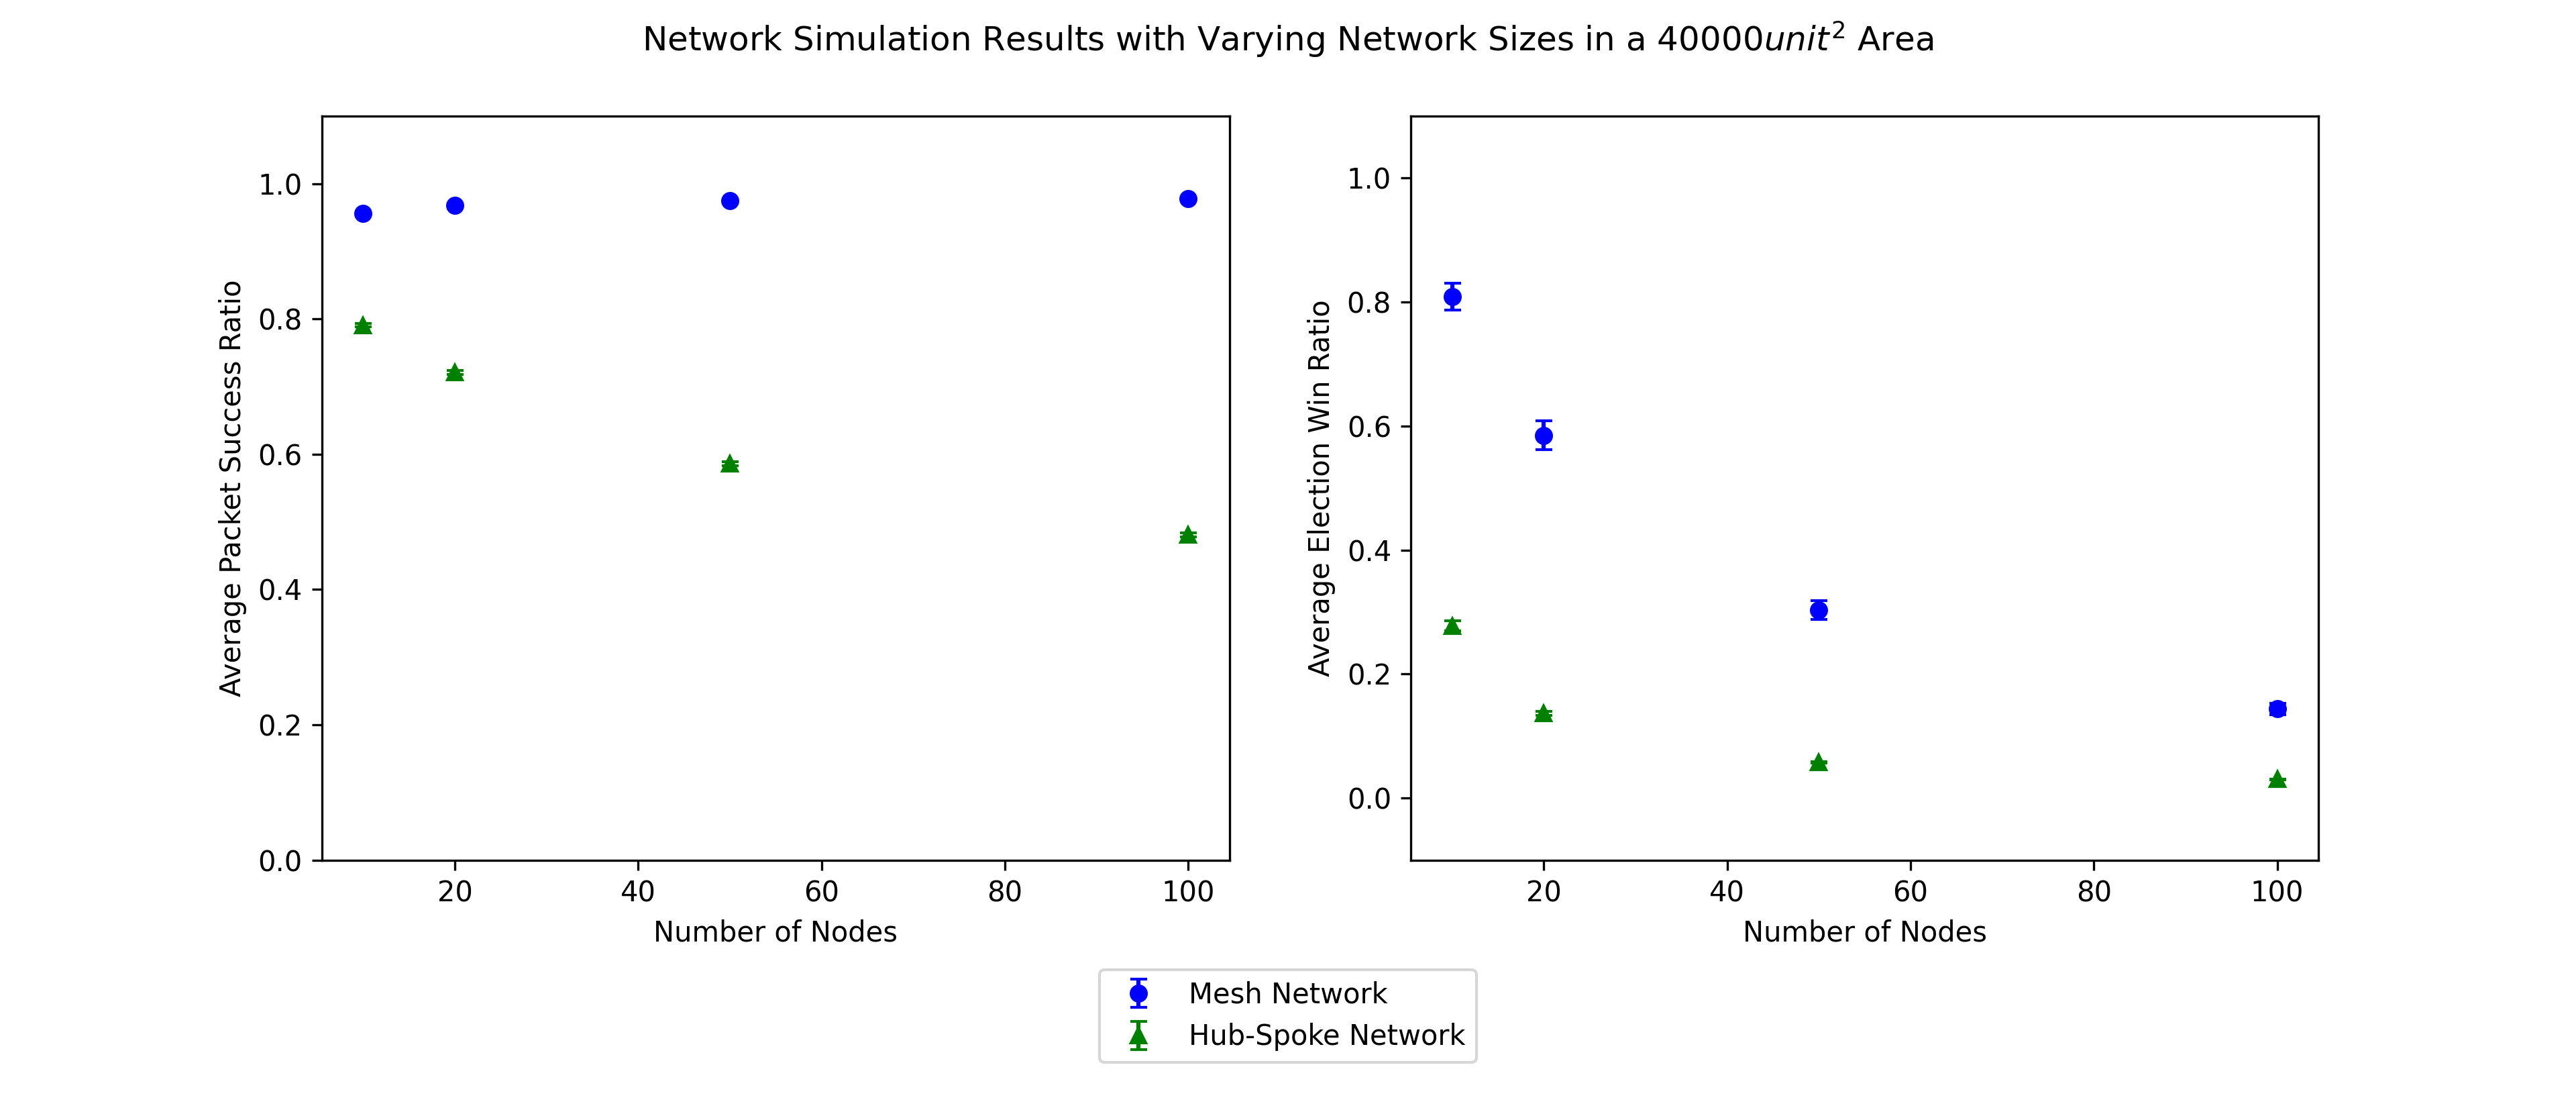
\includegraphics[width=0.9\columnwidth]{images/200unit^2.png}
    \caption{Left: Average packet delivery success ratio per number of nodes, Right: Average ratio of elections won to initiated per number of nodes }
    \label{fig:simulation_result_200}
\end{figure}


\begin{figure}[H]
    \centering
    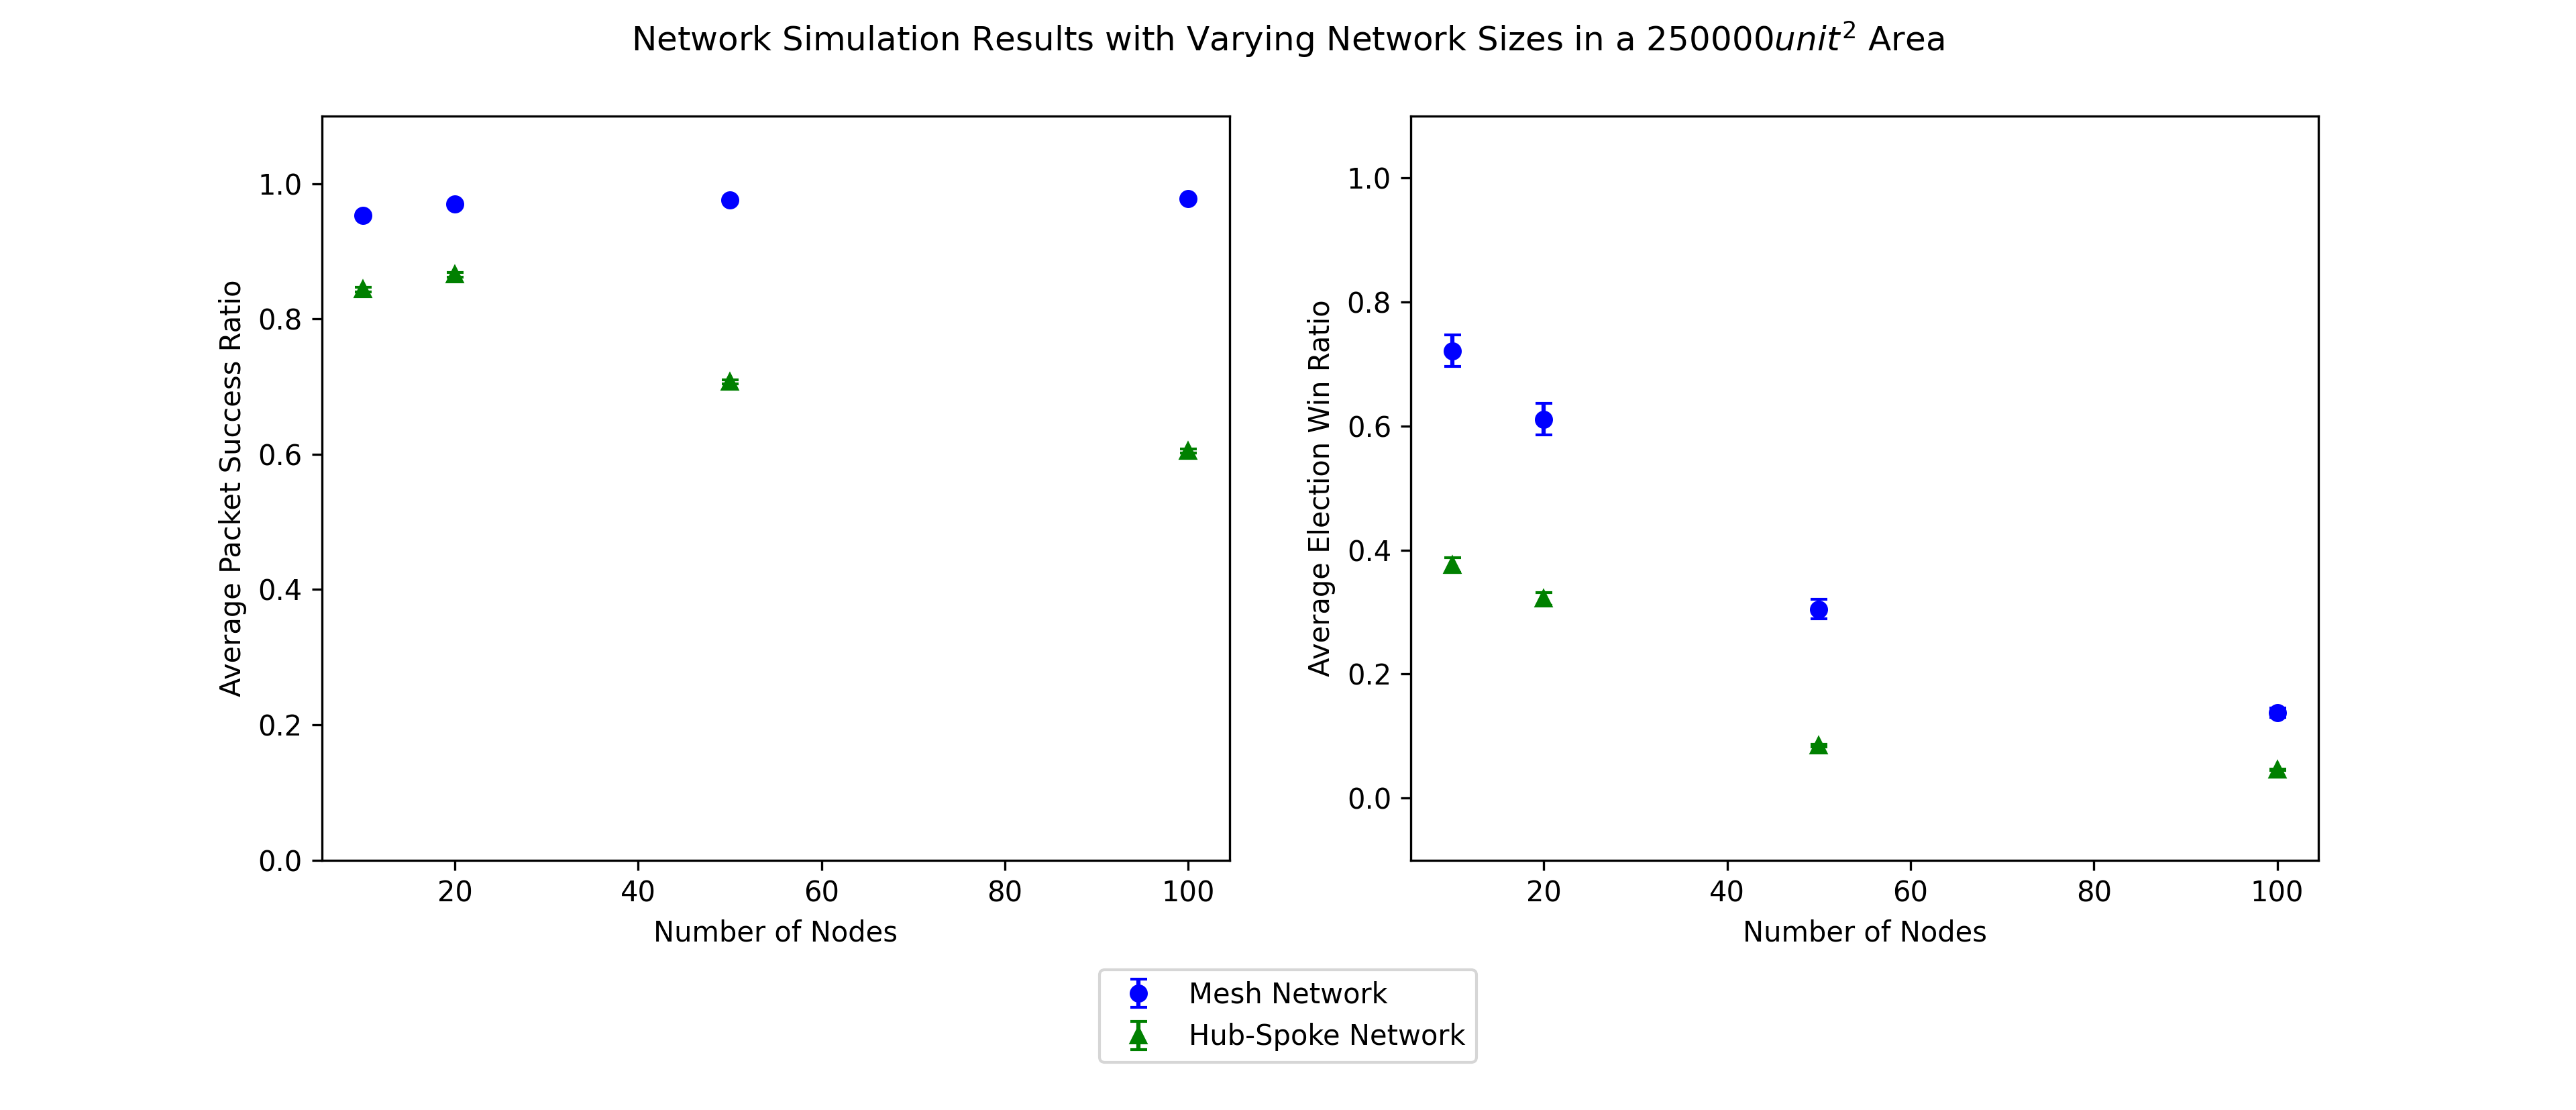
\includegraphics[width=0.9\columnwidth]{images/500unit^2.png}
    \caption{Left: Average packet delivery success ratio per number of nodes, Right: Average ratio of elections won to initiated per number of nodes }
    \label{fig:simulation_result_500}
\end{figure}

\end{document}